\documentclass{report}

\usepackage{vub}
%% PACKAGES

% Fancy chapters with toc
\usepackage{titlesec,titletoc}

\usepackage[style=alphabetic, maxnames=4]{biblatex}
\addbibresource{references.bib}

\usepackage{amsmath,amsfonts,amsthm,amssymb,mathtools}
\usepackage[shortlabels]{enumitem}
\usepackage{imakeidx}
\makeindex[intoc] % Add index to bibliography.
\usepackage[bookmarksdepth=2]{hyperref}
\usepackage{xcolor}
\hypersetup{
	colorlinks=true,
	linkcolor={red!50!black},
	citecolor={blue!50!black},
	urlcolor={blue!80!black}
}
\usepackage{cleveref}
\usepackage{tikz-cd}
\usepackage{aligned-overset}
\usepackage{tcolorbox}
\tcbuselibrary{breakable}
% \tcbuselibrary{theorems}
\tcbuselibrary{skins}
\usepackage{microtype}
\usepackage{nicematrix}
\NiceMatrixOptions{cell-space-limits = 5pt}

\renewcommand{\thechapter}{\Roman{chapter}}
\counterwithout{section}{chapter}
\counterwithout{figure}{chapter}
\counterwithout{table}{chapter}
\renewcommand*\thesection{\arabic{section}}

\titleformat{\chapter}[display]
{\bfseries\Large}
{\filleft
	\MakeUppercase{\chaptertitlename} \Huge\thechapter}
{3ex}
{\titlerule
	\vspace{2ex}%
	\filright}
[{%
			\vspace{2ex}%
			\titlerule
		}]

\titlecontents{chapter}
[0pt]
{\addvspace{1pc}}%
{\contentsmargin{0pt}%
	\bfseries
	\makebox[0pt][r]{\huge\thecontentslabel\enspace}%
	\large}
{% \addvspace{.2pc}%
	\contentsmargin{0pt}%
	\large}
{}
[\addvspace{.5pc}]

\newcommand{\chaptertoc}{%
	\dotfill
	\vspace*{1ex}
	\startcontents[chapters]
	\printcontents[chapters]{}{1}[2]{}
	\vspace*{1ex}
	\noindent\dotfill\\
	\vspace*{1pc}
}
% \usepackage{fancyhdr}
% \pagestyle{fancy}

\usetikzlibrary{positioning,quotes,calc,patterns}

%% Equation numbered by section
\numberwithin{equation}{section}

%% Theorem environments
\theoremstyle{plain}
\newtheorem{theorem}{Theorem}[section]
\newtheorem{lemma}[theorem]{Lemma}
\newtheorem{proposition}[theorem]{Proposition}
\newtheorem{corollary}[theorem]{Corollary}

\newtheorem{condition}{Condition}
\renewcommand*{\thecondition}{\Alph{condition}}
\crefname{condition}{condition}{conditions}

\newtheorem*{convention}{Convention}
\newtheorem*{theorem*}{Theorem}
\newtheorem*{lemma*}{Lemma}
\newtheorem*{prop*}{Proposition}
\newtheorem*{corollary*}{Corollary}

\theoremstyle{definition}
\newtheorem{definition}[theorem]{Definition}
% \newtheorem{example}[theorem]{Example}
\newtheorem{exercise}[theorem]{Exercise}
\newtheorem*{notation}{Notation}
\newtheorem*{definition*}{Definition}
\newtheorem*{example*}{Example}
\newtheorem*{exercise*}{Exercise}

\theoremstyle{remark}
\newtheorem{remark}[theorem]{Remark}
\newtheorem*{remark*}{Remark}

\tcolorboxenvironment{notation}{%
	blanker,breakable,left=5mm,
	before skip=10pt,after skip=10pt,
	borderline west={1mm}{0pt}{gray}}

\usepackage{thmtools}

\declaretheoremstyle[
  sibling=theorem,
	style=definition,
  spaceabove=1em plus 0.75em minus 0.25em,
  spacebelow=1em plus 0.75em minus 0.25em,
  qed={\itshape End of example.}
]{exmpstyle}

\declaretheorem[
  style=exmpstyle,
  title=Example,
  refname={example,examples},
  Refname={Example,Examples}
]{example}

%===========================================================%
%The code below customises theorem numbering
%===========================================================%

% \theoremstyle{plain}
% \newtheorem{innercustomgenericplain}{\customgenericname}
% \providecommand{\customgenericname}{}
% \newcommand{\newcustomtheoremplain}[2]{%
% 	\crefname{#2}{#2}{#2s}%
% 	\newenvironment{#1}[1]
% 	{%
% 		\renewcommand\customgenericname{#2}%
% 		\crefalias{innercustomgenericplain}{#2}%
% 		\renewcommand\theinnercustomgenericplain{##1}%
% 		\innercustomgenericplain
% 	}
% 	{\endinnercustomgenericplain}
% }

% \theoremstyle{definition}
% \newtheorem{innercustomgenericdefinition}{\customgenericname}
% \providecommand{\customgenericname}{}
% \newcommand{\newcustomtheoremdefinition}[2]{%
% 	\crefname{#2}{#2}{#2s}%
% 	\newenvironment{#1}[1]
% 	{%
% 		\renewcommand\customgenericname{#2}%
% 		\crefalias{innercustomgenericdefinition}{#2}%
% 		\renewcommand\theinnercustomgenericdefinition{##1}%
% 		\innercustomgenericdefinition
% 	}
% 	{\endinnercustomgenericdefinition}
% }

% \theoremstyle{remark}
% \newtheorem{innercustomgenericremark}{\customgenericname}
% \providecommand{\customgenericname}{}
% \newcommand{\newcustomtheoremremark}[2]{%
% 	\crefname{#2}{#2}{#2s}%
% 	\newenvironment{#1}[1]
% 	{%
% 		\renewcommand\customgenericname{#2}%
% 		\crefalias{innercustomgenericremark}{#2}%
% 		\renewcommand\theinnercustomgenericremark{##1}%
% 		\innercustomgenericremark
% 	}
% 	{\endinnercustomgenericremark}
% }

% \newcustomtheoremplain{customtheorem}{Theorem}
% \newcustomtheoremplain{customlemma}{Lemma}
% \newcustomtheoremplain{customprop}{Proposition}
% \newcustomtheoremplain{customcorollary}{Corollary}

% \newcustomtheoremdefinition{customdefinition}{Definition}
% \newcustomtheoremdefinition{customexample}{Example}
% \newcustomtheoremdefinition{customexercise}{Exercise}

% \newcustomtheoremremark{customremark}{Remark}

\input{definitions/macros}
\input{definitions/letterfonts}

\includeonly{
	contents/01-classical,
	contents/02-quantum
}

\usetikzlibrary{shapes.geometric,calc, decorations.pathmorphing, arrows.meta}

\newcommand{\ex}{\mathbf{ex}}
\newcommand{\frz}{\mathbf{frz}}
\newcommand{\bx}{\mathbf{x}}
\newcommand{\tbx}{\tilde{\bx}}
\newcommand{\tB}{\tilde{B}}
\newcommand{\blambda}{\boldsymbol{\lambda}}
\DeclareMathOperator{\Fract}{Fract}
\DeclareMathOperator{\id}{id}

%%%%%%%%%%%%%
%% Fill in!%%
%%%%%%%%%%%%%
\title{Cluster Algebras}
\subtitle{Collection of notes on (quantum) cluster algebras}
\faculty{Sciences and Bio-Engineering Sciences}
\author{Wannes Malfait}
\date{Academic year 2023-2024}
\promotors{Kenny De Commer, Geoffrey Janssens}
% \pretitle{Dissertation for the grade of Master's in mathematics}

\begin{document}

\maketitle
\newpage
\tableofcontents
\newpage

\chapter{Classical cluster algebras}
Mostly use \cite{FominWilliams2021IntroductionCA_1-3} as reference together with
Geoffrey's notes.

\section{Cluster algebras from quivers}

This first section serves as an introduction to cluster algebras. We will first look at
some examples of integer sequences arising from number theory or from combinatorial
data. In these examples, a few recurring observations will occur. These observations
will be explained by viewing each of the examples under the lens of cluster algebra
theory. We do not yet provide the most general definition of a cluster algebra, which
will instead be done in \cref{sec:ice_quivers_and_coefficients}. Instead, we focus on
the simplest case of a cluster algebra associated to a quiver. This case is easier to
grasp, and allows understanding the general concepts without getting distracted by
technical details.

\subsection{Combinatorial integer sequences}\label{sec:integer_sequences}

Let us start by looking at some integer sequences coming from number theory or
combinatorial data. Along the way we observe some interesting patterns which will be
explained by viewing these sequences as arising from a cluster algebra. \medskip

\begin{example}\label{exmp:markov_sequence}
	Consider the sequence given by the recurrence relation
	\begin{equation*}
		x_{n+3} = \frac{x_{n+1}^2 + x_{n+2}^2}{x_n},
	\end{equation*}
	with initial conditions $x_0 = x_1 = x_2 = 1$. Computing the first few terms gives
	\begin{equation*}
		1,1,1,2,5,29,433,37666,48928105,\dots
	\end{equation*}
	%
	Even though the recurrence relation involves a fraction, all the terms of the sequence
	are positive integers. We will explain this later, as a consequence of a more general
	fact about cluster algebras. Another way to observe this is as follows. For each $n \in
		\bbZ_{\geq0}$, the triple $(x_n, x_{n+1}, x_{n+2})$ satisfies the equation
	\begin{equation}\label{eq:markov_diophantine}
		x_n^2 + x_{n+1}^2 + x_{n+2}^2 = 3 x_n x_{n+1}x_{n+2},
	\end{equation}
	known as the \emph{Markov equation}\index{Markov!equation}\footnote{It is named after Andrey Markov. This is the same mathematician after whom Markov chains are named.}. The case $n = 0$ is clear. Then, by induction, we have
	\begin{equation}\label{eq:markov_mutation_simplified}
		x_{n+3} = \frac{x_{n+1}^2 + x_{n+2}^2}{x_n} = \frac{3 x_n x_{n+1}x_{n+2} - x_n^2}{x_n} = 3 x_{n+1} x_{n+2} - x_n,
	\end{equation}
	so that
	\begin{align*}
		x_{n+3}^2 + x_{n+2}^2 + x_{n+1}^2
		 & = (3 x_{n+1}x_{n+2} - x_n)^2 + x_{n+1}^2 + x_{n+2}^2                            \\
		 & = 9 x_{n+1}^2 x_{n+2}^2 - 6 x_{n+1} x_{n+2} x_n + x_n^2 + x_{n+1}^2 + x_{n+2}^2 \\
		 & = 9 x_{n+1}^2 x_{n+2}^2 - 6 x_n x_{n+1} x_{n+2} + 3 x_n x_{n+1} x_{n+2}         \\
		 & = 9 x_{n+1}^2 x_{n+2}^2 - 3 x_n x_{n+1} x_{n+2}                                 \\
		 & = 3 ( x_{n+1} x_{n+2}-  x_n) x_{n+1} x_{n+2}                                    \\
		 & = 3 x_{n+3} x_{n+1} x_{n+2}.
	\end{align*}
	%
	The intermediate result, \cref{eq:markov_mutation_simplified}, also immediately implies
	that all the terms in the sequence are integers. That they are positive follows from
	the recurrence relation itself.
\end{example}

\begin{example}\label{exmp:somos4}

	Let $a_n$ be the sequence defined through the recurrence relation
	\begin{equation}
		\label{eq:somos_4}
		a_{n+4} = \frac{a_{n+3}a_{n+1}+ a_{n+2}^2}{a_n}
	\end{equation}
	%
	with initial conditions $a_0 = a_1 = a_2 = a_3 = 1$. This sequence is known as the
	\emph{Somos-4}\index{Somos-4 sequence} sequence, named after its inventor, Michael
	Somos. It can be seen as a slight generalization of the sequence from
	\cref{exmp:markov_sequence}. Computing the first few terms of the sequence, we find:
	\begin{align*}
		 & \begin{aligned}
			   a_4 & = \frac{1 \cdot 1 + 1^2}{1} = 2                   \\
			   a_5 & = \frac{2 \cdot 1 + 1^2}{1} = 3                   \\
			   a_6 & = \frac{3 \cdot 1 + 2^2}{1} = 7                   \\
			   a_7 & = \frac{7 \cdot 2 + 3^2}{2} = 23                  \\
			   a_8 & = \frac{23 \cdot 3 + 7^2}{2} = \frac{118}{2} = 59 \\
		   \end{aligned}
		 &
		\begin{aligned}
			a_9    & = \frac{59 \cdot 7 + 23^2}{3} = \frac{942}{3} = 314                       \\
			a_{10} & = \frac{314 \cdot 23 + 59^2}{7} = \frac{10703}{7} = 1529                  \\
			a_{11} & = \frac{1529 \cdot 59 + 314^2}{23} = \frac{188807}{23} = 8209             \\
			a_{12} & = \frac{8209 \cdot 314 + 1529^2}{59} = \frac{4915467}{59} = 83313         \\
			a_{13} & = \frac{83313 \cdot 1529 + 8209^2}{314} = \frac{194773258}{314} = 620297.
		\end{aligned}
	\end{align*}
	%
	Just like in the previous example, there is no reason, a priori, to assume that all the
	elements of the sequence would be integers. However, somewhat remarkably, the
	denominators seem to always cancel out perfectly. Viewing this sequence through the
	cluster algebra framework, it will follow immediately that all the terms are indeed
	integers, as a corollary of the \emph{Laurent phenomenon}\index{Laurent!-phenomenon}.
\end{example}

\begin{example}\label{exmp:frieze_patterns}

	The next family of integer sequences comes from \emph{$\SL_2(\bbZ)$-frieze
		patterns}\footnote{The name ``frieze pattern'' comes from architecture, where it refers
		to a horizontal strip, often found just below the roofline, which is decorated with
		patterns.}\index{frieze pattern}\index{SL 2 Z@$\SL_2(\bbZ)$}. The idea of a frieze
	pattern is best explained through an example (\cite{Coxeter1971FriezePatterns}). Take
	for example the following pattern:
	\begin{equation*}
		\dots\quad
		\begin{tikzcd}[
				sep = 0.2em, cramped,
			]
			&0&&0&&0&&0&&0&&0&&0&&0&&0&&0&&0\\
			1&&1&&1&&1&&1&&1&&1&&1&&1&&1&&1\\
			&1&&2&&2&&3&&1&&2&&4&&1&&2&&2&&3\\
			3&&1&&3&&5&&2&&1&&7&&3&&1&&3&&5\\
			&2&&1&&7&&3&&1&&3&&5&&2&&1&&7&&3\\
			3&&1&&2&&4&&1&&2&&2&&3&&1&&2&&4\\
			&1&&1&&1&&1&&1&&1&&1&&1&&1&&1&&1\\
			0&&0&&0&&0&&0&&0&&0&&0&&0&&0&&0
		\end{tikzcd}
		\quad
		\dots
	\end{equation*}
	The defining property is that the $2 \times 2$ diamonds
	\begin{equation*}
		\begin{matrix}
			  & b &   \\
			a &   & d \\
			  & c &
		\end{matrix}
	\end{equation*}
	formed by adjacent elements, can be seen as an element of $\SL_2 (\bbZ)$, i.e., $ad - bc = 1$. Other than the bounding rows of ones and zeros, there is no additional requirement. In what follows we will omit the irrelevant row of zeros.

	One could ask if it is always possible to construct such a pattern for any number of
	rows. If so, one might be interested in knowing how many such patterns there are.
	Furthermore, one might notice that the pattern is periodic, repeating every 7 columns.
	In fact, the pattern even has ``half-periodicity'' where the marked triangle undergoes
	a translation and reflection.
	\begin{equation*}
		\dots\quad
		\begin{tikzcd}[
				sep = 0.2em, cramped,
				execute at end picture = {
						\draw[blue, dashed, rounded corners]
						($(\tikzcdmatrixname-1-1.north west) + (-0.3, 0.05)$) -- ($(\tikzcdmatrixname-1-11.north east)+ (0.3, 0.05)$)--($(\tikzcdmatrixname-6-6.south) + (0,-0.05)$) -- cycle;
						\draw[red, dashed, rounded corners]
						($(\tikzcdmatrixname-6-8.south west) + (-0.3, -0.05)$) -- ($(\tikzcdmatrixname-6-18.south east)+ (0.3, -0.05)$)--($(\tikzcdmatrixname-1-13.north) + (0,0.05)$) -- cycle;
					}
			]
			1&&1&&1&&1&&1&&1&&1&&1&&1&&1&&1\\
			&1&&2&&2&&3&&1&&2&&4&&1&&2&&2&&3\\
			3&&1&&3&&5&&2&&1&&7&&3&&1&&3&&5\\
			&2&&1&&7&&3&&1&&3&&5&&2&&1&&7&&3\\
			3&&1&&2&&4&&1&&2&&2&&3&&1&&2&&4\\
			&1&&1&&1&&1&&1&&1&&1&&1&&1&&1&&1\\
		\end{tikzcd}
		\quad
		\dots
	\end{equation*}

	To make such a pattern, we start with the observation that the rest of the pattern is
	completely determined by a lattice path from top to bottom. Indeed, using the
	$\SL_2(\bbZ)$ rule, one can fill in the rest of the pattern. For example, say we
	started with the following partially filled in pattern:
	\begin{equation*}
		\dots\quad
		\begin{tikzcd}[
				sep = 0.2em, cramped,
			]
			1&&1&&1&&1&&1&&1&&1\\
			&a\\
			b\\
			&1&&1&&1&&1&&1&&1\\
		\end{tikzcd}
		\quad
		\dots
	\end{equation*}
	then the rest has to be filled out as follows
	\begin{equation*}
		\dots\quad
		\begin{tikzcd}[
				sep = 0.2em, cramped,
			]
			1&&1&&1&&1&&1&&1&&1\\
			&a&& \frac{1+a+b}{ab} && b && \frac{1+a}{b} && \frac{1+b}{a} && a\\
			b&& \frac{1+a}{b} &&  \frac{1+b}{a} && a && \frac{1+a+b}{ab} && b\\
			&1&&1&&1&&1&&1&&1\\
		\end{tikzcd}
		\quad
		\dots
	\end{equation*}
	%
	Since all the denominators are monomials in $a$ and $b$, it follows that when $a = b =
		1$, all the elements will be integers, as required.

	It seems that we somehow got lucky in this case. There is again, a priori, no reason to
	assume that for any number of rows, we will always be able to choose the initial
	integers such that all the fractions simplify. The fact that this is possible, follows
	again from the ``Laurent phenomenon''\index{Laurent!-phenomenon}, on which we can now
	shed a bit more light. Let $a_1, a_2, \dots, a_n$ be the initial integers chosen on the
	lattice path. Then, in this context, the Laurent phenomenon states that all the other
	elements of the frieze pattern can be written as Laurent
	polynomials\index{Laurent!-polynomial} in $a_1 , \dots, a_n$ with coefficients in
	$\bbZ$, i.e., as an element of $\bbZ [a_1 ^\pm, \dots, a_n^\pm]$. So, any lattice path
	from top to bottom consisting of only ones, will yield a frieze pattern. This already
	proves the existence of such frieze patterns for any number of rows. We will return to
	the other questions in \cref{sec:sequences_revisited}.
\end{example}

The last example will be based on the following theorem from Euclidean geometry.
\begin{theorem}[Ptolomy's Theorem]\label{thm:ptolomy}

	Let $A,B,C,D$ be distinct points on a circle, in cyclic order (\cref{fig:ptolomy}).
	These determine vertices of a quadrilateral, where the side, and diagonal lengths
	satisfy the following rule:
	\begin{equation*}
		|AC| \cdot |BD| = |AB|\cdot |CD| + |AD| \cdot |BC|.
	\end{equation*}
\end{theorem}

\begin{figure}
	\centering

	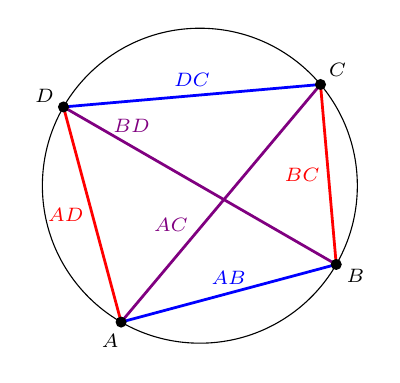
\begin{tikzpicture}
		\coordinate (center) at (0,0);
		\def\radius{2cm}
		\draw (center) circle[radius=\radius];

		% points on the circle
		\path (center) ++(-120:\radius) coordinate (A);
		\path (center) ++(-30:\radius) coordinate (B);
		\path (center) ++(40:\radius) coordinate (C);
		\path (center) ++(150:\radius) coordinate (D);

		\begin{scriptsize}
			% Chords
			\draw[color=red, line width=1pt] (A) -- node[left] {$AD$} (D);
			\draw[color=red, line width=1pt] (B) -- node[left] {$BC$} (C);
			\draw[color=blue, line width=1pt] (A) -- node[above] {$AB$} (B);
			\draw[color=blue, line width=1pt] (D) -- node[above] {$DC$} (C);
			\draw[color=violet, line width=1pt] (A) -- node[above=8pt, near start] {$AC$} (C);
			\draw[color=violet, line width=1pt] (D) -- node[above=2pt, near start] {$BD$} (B);

			% Draw the points over the chords
			\fill[black] (A) circle[radius=2pt] ++(-120:1em) node {$A$};
			\fill[black] (B) circle[radius=2pt] ++(-30:1em) node {$B$};
			\fill[black] (C) circle[radius=2pt] ++(40:1em) node {$C$};
			\fill[black] (D) circle[radius=2pt] ++(150:1em) node {$D$};

		\end{scriptsize}
	\end{tikzpicture}
	\caption{Ptolomy's theorem:
	${\color{violet} |AC| \cdot |BD|}
		= {\color{red} |AD|\cdot |BC|} + {\color{blue} |AB| \cdot |CD|}$.}
	\label{fig:ptolomy}
\end{figure}

\begin{example}\label{exmp:triangulations}

	Note that \cref{thm:ptolomy} allows one to compute the length of one of the diagonals
	in terms of the other, given the side lengths. We will now apply this to triangulations
	of polygons.

	Let $1, 2, \dots, n$ denote $n$ points on a circle, arranged in cyclic order. By
	connecting these points through sides $P_{i, i+1}$, where the indices are taken modulo
	$n$, we obtain a polygon with $n$-sides. A triangulation\index{triangulations!of
		polygons}, $T$, is a choice of $(n-3)$ non-crossing diagonals. This results in a
	partitioning of the polygon in $n-2$ triangles. We will see triangulations in much more
	detail in \cref{sec:triangulations_of_surfaces}, and will therefore keep things brief
	here. For now, it is enough to understand things visually (cf.
	\cref{fig:hexagon_triangulations}).
	\begin{figure}[ht]
		\centering

		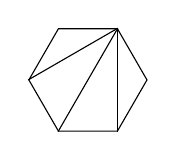
\begin{tikzpicture}
			\node[name=h, shape=regular polygon, draw, regular polygon sides = 6, minimum size = 1.5cm]{};
			\draw[] (h.corner 1) -- (h.corner 3);
			\draw[] (h.corner 1) -- (h.corner 4);
			\draw[] (h.corner 1) -- (h.corner 5);
		\end{tikzpicture}
		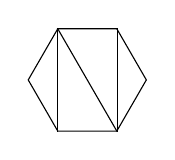
\begin{tikzpicture}
			\node[name=h, shape=regular polygon, draw, regular polygon sides = 6, minimum size = 1.5cm]{};
			\draw[] (h.corner 2) -- (h.corner 5);
			\draw[] (h.corner 2) -- (h.corner 4);
			\draw[] (h.corner 1) -- (h.corner 5);
		\end{tikzpicture}
		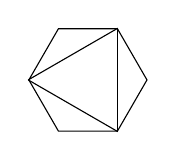
\begin{tikzpicture}
			\node[name=h, shape=regular polygon, draw, regular polygon sides = 6, minimum size = 1.5cm]{};
			\draw[] (h.corner 1) -- (h.corner 3);
			\draw[] (h.corner 3) -- (h.corner 5);
			\draw[] (h.corner 1) -- (h.corner 5);
		\end{tikzpicture}
		\caption{The triangulations of a regular hexagon up to rotation.}
		\label{fig:hexagon_triangulations}
	\end{figure}

	Starting from a triangulation, $T$, we obtain a new triangulation, $T'$, by
	``flipping'' a diagonal. Any diagonal in a triangulation lies on precisely 2 triangles.
	These two triangles form a quadrilateral. To flip the diagonal, you replace it with the
	other diagonal of that quadrilateral. Again, this is most easily seen visually:
	\begin{equation*}
		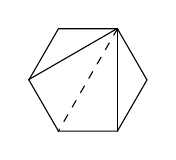
\begin{tikzpicture}[baseline]
			\node[name=h, shape=regular polygon, draw, regular polygon sides = 6, minimum size = 1.5cm]{};
			\draw[] (h.corner 1) -- (h.corner 3);
			\draw[dashed] (h.corner 1) -- (h.corner 4);
			\draw[] (h.corner 1) -- (h.corner 5);
		\end{tikzpicture}
		\quad \leadsto \quad
		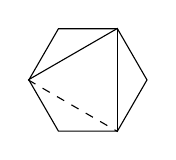
\begin{tikzpicture}[baseline]
			\node[name=h, shape=regular polygon, draw, regular polygon sides = 6, minimum size = 1.5cm]{};
			\draw[] (h.corner 1) -- (h.corner 3);
			\draw[dashed] (h.corner 3) -- (h.corner 5);
			\draw[] (h.corner 1) -- (h.corner 5);
		\end{tikzpicture}
	\end{equation*}
	%
	Using Ptolomy's theorem, the length of the new diagonal can be computed given that we
	knew the lengths of all the edges in the previous triangulation. We now ignore
	Euclidean geometry, and just use Ptolomy's theorem as a recurrence relation to
	construct a collection of numbers as follows. Pick a triangulation and set all the edge
	lengths equal to one. Then at each step, choose a diagonal in the triangulation and
	flip it. Compute its edge length using Ptolomy's theorem. This is the next number in
	the collection. For example, we could obtain a sequence starting like this (we omit the
	ones on the sides):
	\begin{equation*}
		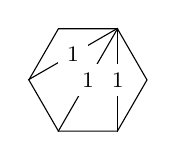
\begin{tikzpicture}[baseline]
			\node[name=h, shape=regular polygon, draw, regular polygon sides = 6, minimum size = 1.5cm]{};
			\draw[] (h.corner 1) -- node[fill=white, font=\footnotesize] {1} (h.corner 3);
			\draw[] (h.corner 1) -- node[fill=white, font=\footnotesize] {1} (h.corner 4);
			\draw[] (h.corner 1) -- node[fill=white, font=\footnotesize] {1} (h.corner 5);
		\end{tikzpicture}
		\leadsto
		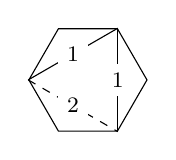
\begin{tikzpicture}[baseline]
			\node[name=h, shape=regular polygon, draw, regular polygon sides = 6, minimum size = 1.5cm]{};
			\draw[] (h.corner 1) -- node[fill=white, font=\footnotesize] {1} (h.corner 3);
			\draw[dashed] (h.corner 3) -- node[fill=white, font=\footnotesize] {2} (h.corner 5);
			\draw[] (h.corner 1) -- node[fill=white, font=\footnotesize] {1} (h.corner 5);
		\end{tikzpicture}
		\leadsto
		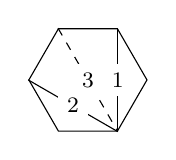
\begin{tikzpicture}[baseline]
			\node[name=h, shape=regular polygon, draw, regular polygon sides = 6, minimum size = 1.5cm]{};
			\draw[dashed] (h.corner 2) -- node[fill=white, font=\footnotesize] {3} (h.corner 5);
			\draw[] (h.corner 3) -- node[fill=white, font=\footnotesize] {2} (h.corner 5);
			\draw[] (h.corner 1) -- node[fill=white, font=\footnotesize] {1} (h.corner 5);
		\end{tikzpicture}
		\leadsto
		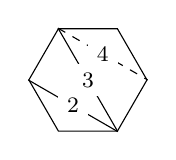
\begin{tikzpicture}[baseline]
			\node[name=h, shape=regular polygon, draw, regular polygon sides = 6, minimum size = 1.5cm]{};
			\draw[] (h.corner 2) -- node[fill=white, font=\footnotesize] {3} (h.corner 5);
			\draw[] (h.corner 3) -- node[fill=white, font=\footnotesize] {2} (h.corner 5);
			\draw[dashed] (h.corner 2) -- node[fill=white, font=\footnotesize] {4} (h.corner 6);
		\end{tikzpicture}
		\leadsto
		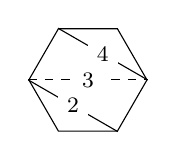
\begin{tikzpicture}[baseline]
			\node[name=h, shape=regular polygon, draw, regular polygon sides = 6, minimum size = 1.5cm]{};
			\draw[dashed] (h.corner 3) -- node[fill=white, font=\footnotesize] {3} (h.corner 6);
			\draw[] (h.corner 3) -- node[fill=white, font=\footnotesize] {2} (h.corner 5);
			\draw[] (h.corner 2) -- node[fill=white, font=\footnotesize] {4} (h.corner 6);
		\end{tikzpicture}
		\leadsto
		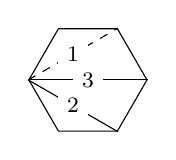
\begin{tikzpicture}[baseline]
			\node[name=h, shape=regular polygon, draw, regular polygon sides = 6, minimum size = 1.5cm]{};
			\draw[] (h.corner 3) -- node[fill=white, font=\footnotesize] {3} (h.corner 6);
			\draw[] (h.corner 3) -- node[fill=white, font=\footnotesize] {2} (h.corner 5);
			\draw[dashed] (h.corner 3) -- node[fill=white, font=\footnotesize] {1} (h.corner 1);
		\end{tikzpicture}
		\leadsto \cdots
	\end{equation*}
	%
	Once again, we observe that we only obtain integers. Furthermore, there seems to be a
	limit to which integers we can obtain this way. This hints at a hidden periodicity. The
	Laurent phenomenon offers an explanation for why we only obtain integers: the lengths
	of the diagonals are Laurent polynomials in the originally chosen lengths.
\end{example}

There are many more examples like the three that we just gave. One can look at wiring
diagrams, generalized Somos sequences, knight recurrence, the Gale-Robinson sequence,
etc. As the focus of this thesis is not on number theory, we refrain from delving
deeper into this interesting world. We refer interested readers to \cite[Chapter
	3.4]{FominWilliams2021IntroductionCA_1-3} and \cite{FominZelevinsky2002Laurent}.

\subsection{Quivers, seeds and mutations}\label{sec:quivers_seeds_mutations}

In the examples from \cref{sec:integer_sequences} we made a couple of observations. In
each case, the sequence consisted of positive integers, something which was not so
obvious from the initial definitions. For
\cref{exmp:frieze_patterns,exmp:triangulations}, we also found some form of finiteness
and periodicity. There are some more subtle similarities, which will be explained in
detail in \cref{sec:sequences_revisited}. Before that, we must introduce the notion of
a cluster algebra. These can be constructed from a quiver, as we now explain.

\begin{definition}[Quivers]

	A \emph{quiver}\index{quiver} is a finite directed (multi)-graph with no 1-cycles
	(vertex connected to itself) or 2-cycles (two vertices connected by a pair of opposite
	arrows) (cf. \cref{fig:quivers}). For a quiver $Q$, we will denote the set of vertices
	with $Q_0$\index{Q 0@$Q_0$}.
\end{definition}

\begin{figure}[ht!]
	\centering
	\begin{equation*}
		\begin{tikzcd}
			&\bullet \arrow[loop] \arrow[r] &\bullet \\
			\bullet \rar & \bullet \arrow[r, bend left] & \bullet \arrow[l, bend left]
		\end{tikzcd}
		\hspace{2cm}
		\begin{tikzcd}[row sep=small]
			&&& \bullet \\
			\bullet \ar[rrrd, bend right]\rar &\bullet  \rar[leftarrow] &\bullet \ar[ru, shift left] \ar[ru, shift right] \ar[rd] \\
			&&& \bullet\\
			\\
			\bullet \ar[rr] && \bullet \ar[ld]\\
			& \bullet \ar[lu]
		\end{tikzcd}
	\end{equation*}
	\caption{The graphs on the left are not quivers, the graphs on the right are.}
	\label{fig:quivers}
\end{figure}

Let us now fix some notation for what follows. Write $[a,b] = \{a, a + 1, \dots, b\}$
for integers $a,b \in \bbZ$, where $[a,b] = \emptyset$ if $a > b$. Fix an integer $N
	\in \bbZ_{\geq 0}$, and a field $\bbK$ of characteristic zero. Finally, let $\mcF =
	\bbK (Y_1, \dots, Y_N)$ be the \emph{field of rational functions}\index{rational
	function field} over $\bbK$, in $N$ variables. Thus, $\mcF$ consists of fractions $P/Q$
where $P, Q\in \bbK[Y_1, \dots, Y_N]$ are polynomials in the variables $Y_1, \dots,
	Y_N$, and $Q$ is non-zero. In most cases we will take $\bbK = \bbC$ or $\bbK = \bbQ$.
This does not impact the definitions that follow in a meaningfull way.

\begin{definition}
	We call a pair $(Q, \bx)$ a \emph{labeled seed}\index{seed!labeled} if
	\begin{enumerate}
		\item $Q$ is a quiver with vertices $Q_0 = [1, N]$.
		\item $\bx = \{x_1, \dots, x_N\}$ is a \emph{free generating set} of $\mcF$. That is, $\bx$ is a set of $N$ algebraically independent elements that generate $\mcF$.
	\end{enumerate}
	The set $\bx$ will be referred to as the \emph{cluster}\index{cluster}. The elements of $\bx$ will be called \emph{cluster variables}\index{cluster!variable}.
\end{definition}
%
One can also talk about \emph{unlabeled seeds}\index{seed!unlabeled}. An unlabeled seed
is an equivalence class of labeled seeds which are equal up to a simultaneous
re-indexing of the quiver vertices and the cluster variables. We will not need
unlabeled seeds as much, and will hence adopt the following convention.
\begin{convention}
	From now on, when we say \emph{seed}, we will always mean a labeled seed.
\end{convention}

Just like in nature, a seed on it own is not so interesting. We are interested in what
one can obtain from the seed. From a given seed, we can make another seed through a
process known as \emph{seed mutation}\index{seed!mutation}.
\begin{definition}

	Let $k \in \ex$ be an exchangeable vertex of the quiver $Q$. We define the
	\emph{mutation in direction $k$} of the seed $(Q, \bx)$ to be the seed $\mu_k(Q, \bx)
		\defeq (Q', \bx') = (\mu_k(Q), \mu_k(\bx))$\index{mu k@$\mu_k$}, where
	\begin{enumerate}
		\item $Q'_0 \defeq Q_0$.
		\item For every pair of vertices $i,j$ with $s$ arrows $i \to k$ and $t$ arrows $k \to j$ we
		      ``collapse'' these arrows into $s\cdot t$ arrows $i \to j$, cancelling pairwise with
		      any arrows $j \to i$.
		      \begin{equation*}
			      \begin{tikzcd}[column sep=small]
				      i \ar[rr, "r"] \ar[rd, "s"] && j \\
				      & k \ar[ur, "t"]
			      \end{tikzcd}
			      \quad \begin{tikzcd}
				      \; \rar[rightsquigarrow, "\mu_k"]& \;
			      \end{tikzcd}\quad
			      \begin{tikzcd}[column sep=small]
				      i \ar[rr, "r + st"] \ar[rd,leftarrow, "s"] && j \\
				      & k \ar[ur, leftarrow, "t"]
			      \end{tikzcd}
		      \end{equation*}
		      Here we take $r$ to be negative, if the arrows actually point the other way, as the path $i \to k \to j$.
		\item All arrows in $Q$ starting or ending in $k$ get their orientation flipped.
		\item $\bx' = \{x_1', \dots, x_N'\}$, where $x_i' = x_i$ for $i \neq k$, and $x'_k$
		      is given by the \emph{exchange relation}\index{exchange relation}
		      \begin{equation}\label{eq:exchange_relation_quiver}
			      x'_k \defeq \frac{1}{x_k} \left(\prod_{i \to k} x_i + \prod_{k \to j} x_j\right),
		      \end{equation}
		      where we take the product equal to 1 if $\{i \to k\} = \emptyset$ or $\{k \to j\} = \emptyset$.
	\end{enumerate}
\end{definition}

Let us first look at an example involving only the mutation of the quiver.
\begin{example}
	We mutate the given quiver at vertex 2:
	\begin{equation*}
		\begin{tikzcd}
			& 4 \dlar \rar & 6 \dar \\
			1 \rar & 2 \uar \rar \dar[shift left] \dar [shift right] & 5 \\
			& 3 \ular
		\end{tikzcd}
		\begin{tikzcd}
			\; \rar[rightsquigarrow, "\mu_2"] &\;
		\end{tikzcd}
		\begin{tikzcd}
			& 4 \rar \dar & 6 \dar \\
			1  \drar \ar[rr,controls = {+(1, -2) and +(-1, -2)}] & 2 \lar & 5 \lar \\
			& 3 \uar[shift right] \uar[shift left]
		\end{tikzcd}
	\end{equation*}
	%
	The arrow $1 \to 2$ combined with the arrow $2 \to 4$ introduces one new arrow $1 \to
		4$ which cancels out the existing arrow $4 \to 1$. The arrow $1 \to 2$ combines with
	the 2 arrows $2 \to 3$ to create 2 new arrows $1 \to 3$, one of which cancels out with
	the existing arrow $3 \to 1$. Finally, the arrow $1 \to 2$ combined with the arrow $2
		\to 5$ yields an arrow $1 \to 5$. The arrows starting or ending in the vertex 6 remain
	unchanged.
\end{example}

Before we give some examples of seed mutation, we prove a small lemma, which will also
be useful for the examples.
\begin{lemma}\label{lem:mutation_involution}
	Seed mutation at a fixed vertex is an \emph{involution}\index{involution}, i.e., $\mu_k \circ \mu_k = id$.
\end{lemma}

\begin{proof}
	We first show that the quiver remains unchanged. For arrows incident to $k$, the
	mutation reverses the orientation. So, applying it twice yields the same orientation.
	Now, the only other part of the quiver that changes is at pairs of vertices $i,j$ with
	$s$ arrows $i \to k$ and $t$ arrows $k \to j$. Applying a single mutation introduces
	$s\cdot t$ new arrows $i \to j$. When applying the mutation the second time, we now
	have $s$ arrows $k \to i$ and $t$ arrows $j \to k$, due to the orientation flip of the
	arrows incident to $k$. Consequently, the mutation introduces $s \cdot t$ arrows $j \to
		i$ which cancel out exactly the arrows from the first mutation.

	That the cluster variables remain unchanged is a simple calculation:
	\begin{align*}
		x_k''
		 & = \frac{1}{x_k'}\left(\prod_{k \to i}x_i' + \prod_{j \to k} x_j'\right)                                                \\
		 & = x_k \left(\prod_{i \to k} x_i + \prod_{k \to j}x_j\right)^{-1} \left(\prod_{k \to i}x_i + \prod_{j \to k} x_j\right) \\
		 & = x_k,
	\end{align*}
	where we use that the exchange rule is unchanged by an orientation flip of all the arrows.
\end{proof}

\begin{example}
	The simplest example is the seed $(Q, \bx)$ where $Q$ is the quiver consisting of a single vertex:
	\begin{equation*}
		Q = \begin{tikzcd}
			\bullet
		\end{tikzcd},
		\quad \bx = \{x\}.
	\end{equation*}
	%
	Mutating at the only vertex gives
	\begin{equation*}
		Q = \begin{tikzcd}
			\bullet
		\end{tikzcd},
		\quad \bx = \left\{\frac{2}{x}\right\}.
	\end{equation*}
	%
	If we mutate again, we end up with the original seed, as a consequence of
	\cref{lem:mutation_involution}. It is of course also straightforward to verify it
	directly.
\end{example}
\begin{example}\label{exmp:A2_quiver}
	The next simplest example is the $A_2$ quiver\index{quiver!$A_2$}:
	\begin{equation*}
		Q = \begin{tikzcd}
			1 \rar &2
		\end{tikzcd},
		\quad \bx = \left\{x_1, x_2\right\}.
	\end{equation*}
	%
	If we apply a mutation at the first vertex, we obtain:
	\begin{equation*}
		\mu_1(Q) = \begin{tikzcd}
			1 & \lar 2
		\end{tikzcd},
		\quad \mu_1(\bx) = \left\{\frac{1+x_2}{x_1}, x_2\right\}.
	\end{equation*}
	%
	We already know that mutating at the first vertex again will yield the same seed, so
	the only interesting thing to do is to see what happens after mutating at index 2:
	\begin{equation*}
		\mu_2(\mu_1(Q)) = \begin{tikzcd}
			1 \rar & 2
		\end{tikzcd},
		\quad  \mu_2(\mu_1(\bx)) = \left\{\frac{1+x_2}{x_1}, \frac{x_1 + x_2 + 1}{x_1 x_2}\right\}.
	\end{equation*}
	%
	Although we are back at the original quiver, the cluster variables are completely
	different. We now mutate again at the first vertex. We will use the notation
	$\mu_{k_1k_2\cdots k_l}$ as a shorthand for $\mu_{k_l} \circ \cdots \circ \mu_{k_2}
		\circ \mu_{k_1}$.
	\begin{equation*}
		\mu_{121}(Q) = \begin{tikzcd}
			1 &\lar 2
		\end{tikzcd},
		\quad  \mu_{121}(\bx) = \left\{\frac{x_1(x_1 x_2 + x_1 + x_2 + 1)}{x_1x_2(1+x_2)}, \frac{x_1 + x_2 + 1}{x_2}\right\}.
	\end{equation*}
	%
	The expression for the first cluster variable looks complicated, but can be
	dramatically simplified to $\frac{x_1 + 1}{x_2}$. We continue mutating:
	\begin{equation*}
		\mu_{1212}(Q) = \begin{tikzcd}
			1 \rar& 2
		\end{tikzcd},
		\quad  \mu_{1212}(\bx) = \left\{\frac{x_1 + 1}{x_2}, x_1\right\}.
	\end{equation*}
	%
	Once again, some simplification has taken place. We mutate a final time at the first
	vertex.
	\begin{equation*}
		\mu_{12121}(Q) = \begin{tikzcd}
			1 &\lar 2
		\end{tikzcd},
		\quad  \mu_{12121}(\bx) = \left\{x_2, x_1\right\}.
	\end{equation*}

	We have our original seed, except that the arrow in the quiver has been reversed, and
	that $x_1$ and $x_2$ have swapped places. In other words, after 5 mutations, the roles
	of 1 and 2 have swapped. It follows that another 5 swaps will give back the original
	seed.

	If one takes a close look at the obtained cluster variables, then we see that these
	correspond exactly to those that we found when trying to construct a frieze pattern
	with 2 rows (cf. \cref{exmp:frieze_patterns}). This is no coincidence, and we will come
	back to this in \cref{sec:sequences_revisited}.
\end{example}

\begin{example}
	The logical follow-up to the $A_2$ quiver is the $A_3$ quiver\index{quiver!$A_3$}
	\begin{equation*}
		Q =
		\begin{tikzcd}
			1 \rar[] & 2 \rar[] &3
		\end{tikzcd},
		\quad \bx = \left\{x_1, x_2, x_3\right\}.
	\end{equation*}
	Mutation in direction 2 gives
	\begin{equation*}
		\mu_2(Q) =
		\begin{tikzcd}
			1 \rar[leftarrow] \ar[rr, bend right] & 2 \rar[leftarrow]& 3
		\end{tikzcd},
		\quad \mu_2(\bx) = \left\{x_1, \frac{x_1 + x_3}{x_2}, x_3\right\}.
	\end{equation*}
	If we instead apply a mutation in direction 1, we find
	\begin{equation*}
		\mu_1(Q) =
		\begin{tikzcd}
			1 \rar[leftarrow] & 2 \rar[]& 3
		\end{tikzcd},
		\quad \mu_1(\bx) = \left\{\frac{x_2 + 1}{x_1}, x_2, x_3\right\}.
	\end{equation*}
	Finally, a mutation in direction 3 would give
	\begin{equation*}
		\mu_3(Q) =
		\begin{tikzcd}
			1 \rar[] & 2 \rar[leftarrow]& 3
		\end{tikzcd},
		\quad \mu_3(\bx) = \left\{x_1, x_2, \frac{x_2 + 1}{x_3}\right\}.
	\end{equation*}
	Mutating in direction 1 on $\mu_2(Q)$ gives
	\begin{equation*}
		\mu_{21}(Q) =
		\begin{tikzcd}
			1 \rar[] \ar[rr,leftarrow, bend right] & 2 & 3
		\end{tikzcd},
		\quad \mu_{21}(\bx) = \left\{\frac{x_1 + x_3 + x_2x_3}{x_1x_2}, \frac{x_1 + x_3}{x_2}, x_3\right\}.
	\end{equation*}
	If we now mutate in direction 3, we obtain
	\begin{equation*}
		\mu_{213}(Q) =
		\begin{tikzcd}
			1 \rar[] \ar[rr, bend right] & 2 & 3
		\end{tikzcd},
		\quad \mu_{213}(\bx) = \left\{\frac{x_1 + x_3 + x_2x_3}{x_1x_2}, \frac{x_1 + x_3}{x_2}, \frac{x_1 x_2 + x_1 + x_3 + x_2 x_3}{x_1x_2x_3}\right\}.
	\end{equation*}
	It seems that the expressions keep getting messier and messier. We mutate again in direction 2:
	\begin{equation*}
		\mu_{2132}(Q) =
		\begin{tikzcd}
			1 \rar[leftarrow] \ar[rr, bend right] & 2 & 3
		\end{tikzcd},
	\end{equation*}
	\begin{equation*}
		\mu_{2132}(\bx)= \left\{\frac{x_1 + x_3 + x_2x_3}{x_1x_2}, \frac{x_2 + 1}{x_1}, \frac{x_1 x_2 + x_1 + x_3 + x_2 x_3}{x_1x_2x_3}\right\}.
	\end{equation*}
	Somehow, some miraculous cancelation happened.
	Note that the expression $\frac{x_2 + 1}{x_2}$ already appeared previously.
	If we instead mutate in direction 1, we get
	\begin{equation*}
		\mu_{2131}(Q) =
		\begin{tikzcd}
			1 \rar[leftarrow] \ar[rr,leftarrow, bend right] & 2 & 3
		\end{tikzcd},
	\end{equation*}
	\begin{equation*}
		\mu_{2131}(\bx) = \left\{\frac{x_1 + x_3 + x_1x_2}{x_2x_3}, \frac{x_1 + x_3}{x_2}, \frac{x_1 x_2 + x_1 + x_3 + x_2 x_3}{x_1x_2x_3}\right\}.
	\end{equation*}
	This still introduces a new expression.
	Interestingly, these are all the possible expressions we can obtain!
	If we now mutate in, say, direction 3, we would get as cluster
	\begin{equation*}
		\mu_{21313} = \left\{\frac{x_1 + x_3 + x_1x_2}{x_2x_3}, \frac{x_1 + x_3}{x_2}, x_1 \right\}.
	\end{equation*}
	This is again a dramatic cancelation. One can check manually
	that no mutations introduce new cluster variables.
\end{example}

\begin{example}\label{exmp:markov_quiver}
	As a last example, we look at the \emph{Markov quiver}\index{quiver!Markov}\index{Markov!quiver}:
	\begin{equation*}
		\begin{tikzcd}[column sep= small]
			& 1 \ar[ld, shift left] \ar[ld, shift right]\\
			2 \ar[rr, shift left] \ar[rr, shift right] && 3 \ar[lu, shift left] \ar[lu, shift right]
		\end{tikzcd},
	\end{equation*}
	%
	which possesses the special property that it remains invariant under mutations at any
	vertex (up to a simultaneous flipping of all the arrows). Let us see what happens to
	the cluster variables as we mutate in a cyclic order of the vertices. Denote for
	brevity $x \defeq x_1, y \defeq x_2$ and $z \defeq x_3$ for the cluster variables
	corresponding to the vertices $1,2$ and $3$ respectively. Because the exchange relation
	is invariant under a flipping of all the arrows and the Markov quiver is rotationally
	symmetric, the exchange relation will always be of the form
	\begin{equation}\label{eq:markov_exchange_relation}
		w' = \frac{u^2 + v^2}{w},
	\end{equation}
	%
	where $u, v$ and $w$ are the cluster variables of the seed being mutated. Thus, we
	obtain
	\begin{align*}
		\bx            & = \{x, y, z\}                                                                                                                                                                               \\
		\mu_1(\bx)     & = \left\{\frac{y^2 + z^2}{x}, y, z\right\}                                                                                                                                                  \\
		\mu_{12}(\bx)  & = \left\{\frac{y^2 + z^2}{x}, \frac{y^4 + 2 z^2y^2 +z^4 + z^2x^2 }{x^2y}, z\right\}                                                                                                         \\
		\mu_{123}(\bx) & = \left\{\frac{y^2 + z^2}{x}, \frac{y^4 + 2 z^2y^2 +z^4 + z^2x^2 }{x^2y},\right.                                                                                                            \\
		               & \left. \frac{x^{4} z^{4} + x^{2} y^{6} + 4 x^{2} y^{4} z^{2} + 5 x^{2} y^{2} z^{4} + 2 x^{2} z^{6} + y^{8} + 4 y^{6} z^{2} + 6 y^{4} z^{4} + 4 y^{2} z^{6} + z^{8}}{x^{4} y^{2} z} \right\}
	\end{align*}
	%
	Mutating again at the first vertex gives the new cluster variable
	\begin{align*}
		 & \frac{x^{8} z^{6} + 4 x^{6} y^{4} z^{4} + 8 x^{6} y^{2} z^{6} + 4 x^{6} z^{8} + x^{4} y^{10} + 8 x^{4} y^{8} z^{2} + 24 x^{4} y^{6} z^{4} + 34 x^{4} y^{4} z^{6} + 23 x^{4} y^{2} z^{8}}{x^7y^4z^2} \\&+ \frac{6 x^{4} z^{10} + 2 x^{2} y^{12} + 14 x^{2} y^{10} z^{2} + 40 x^{2} y^{8} z^{4} + 60 x^{2} y^{6} z^{6} + 50 x^{2} y^{4} z^{8} + 22 x^{2} y^{2} z^{10} + 4 x^{2} z^{12}}{x^7 y^4 z^2}\\ &+ \frac{y^{14} + 7 y^{12} z^{2} + 21 y^{10} z^{4} + 35 y^{8} z^{6} + 35 y^{6} z^{8} + 21 y^{4} z^{10} + 7 y^{2} z^{12} + z^{14}}{x^{7} y^{4} z^{2}}.
	\end{align*}
	%
	Because the author does not want to spend too much time fiddling with alignment points
	to get long fractions to fit on a page, we will stop here. Mutating at vertex 2 would
	yield another fraction with 65 terms (with positive integer coefficients) in the
	numerator, and the expression $x^{12}y^7z^4$ in the denominator.

	Unlike the previous examples, the cluster variables do not simplify. In fact, one can
	show, that the number of cluster variables is infinite (cf.
	\cref{thm:cluster_finite_classification}). This is in contrast to the quiver itself,
	whose only mutation corresponds to a reversal of all the arrows.
\end{example}

\subsection{The cluster algebra}

From the examples of \cref{sec:quivers_seeds_mutations} we gather the following
observations:
\begin{enumerate}
	\item Even though a sequence of mutations might result in the same quiver, the corresponding
	      cluster variables might be different.
	\item For some quivers, the number of obtainable cluster variables is finite.
	\item Independent of the quiver, all the cluster variables are Laurent polynomials in the
	      original cluster variables.
	\item The Laurent polynomials have coefficients in the positive integers.
\end{enumerate}

To have the correct setting to explain the above observations, we must introduce the
notion of a \emph{cluster algebra}\index{cluster!algebra}\index{algebra!cluster}. From
\cref{lem:mutation_involution} it follows that the process of applying mutations is
invertible. This means that we get a well-defined notion of
\emph{mutation-equivalence}\index{mutation!-equivalence} of seeds. Two seeds are
\emph{equivalent}\index{seed!equivalent} if one can be obtained from the other through
a sequence of mutations.
\begin{definition}

	Choose some \emph{initial seed}\index{seed!initial} $(Q, \bx)$. The \emph{cluster
		algebra} $\mcA (Q, \bx)$\index{A Q x@$\mcA(Q, \bx)$} is the subalgebra of $\mcF$
	generated by all cluster variables $\bx'$ for seeds $(Q', \bx')$ mutation-equivalent to
	the initial seed $(Q, \bx)$.
\end{definition}
\begin{remark}

	Note that the definition of the cluster algebra only depends on the equivalence class
	of a seed.
\end{remark}

The first two observations are about two notions of ``finiteness'' of cluster algebras.
When there are only finitely many mutation-equivalent quivers, we say that the cluster
algebra is \emph{mutation-finite}\index{mutation!-finite}. When there are only finitely
many cluster variables, we say that the cluster algebra is
\emph{cluster-finite}\index{cluster!-finite}\footnote{It is also common to say that a
	cluster algebra is of finite type instead of calling it cluster-finite.}.

Mutation-finite cluster algebras need not be cluster-finite. For example, the Markov
quiver (\cref{exmp:markov_quiver}) is mutation-finite but has infinitely many cluster
variables. The inverse implication is true. Any cluster-finite cluster algebra is
automatically also mutation-finite. Indeed, suppose that there are finitely many
cluster variables, but infinitely many distinct quivers. By the pigeonhole principle,
there is some cluster which appears in infinitely many seeds. Since there are only
finitely many variables in the cluster, one of them has to appear in an infinite number
of exchange rules, but that leads to infinitely many new cluster variables.

Remarkably, it is possible to classify the cluster- and mutation-finite cluster
algebras. To state the classification more precisely, the following lemma is useful:
\begin{lemma}

	Let $Q$ be an unoriented finite tree. Then any two orientations of $Q$ are
	mutation-equivalent through mutations at only sources and sinks. Recall that a
	\emph{source}\index{source} is a vertex such that all arrows incident to the vertex
	point away from the vertex, while a \emph{sink}\index{sink} is a vertex such that all
	incident arrows point to the vertex.
\end{lemma}

\begin{proof}
	We prove this by induction on the number of vertices in $Q$. When $Q$ consists of just a single vertex, there is nothing to prove. Now assume that the statement holds for any tree with $n$ vertices, and let $Q$ be an unoriented tree with $n+1$ vertices. Fix an orientation of $Q$, and let $Q'$ be another orientation of $Q$. Since $Q$ is a tree, it has a leaf $v$, (a vertex of degree 1). Performing a mutation at $v$ only flips the orientation of the single arrow connected to it. Furthermore, it is always a source or a sink.

	Now, consider the subgraph of $Q_v$ obtained by removing $v$ and the arrow connected to
	it. This is a tree with $n$ vertices, and we can hence transform it, by induction, to
	the orientation $Q'_v$ by only mutating at sources and sinks. Write $w$ for the other
	vertex connected to $v$ in $Q$. Applying the same mutations to $Q$ instead of $Q_v$
	would yield the desired orientation for all the arrows, except possibly the arrow
	between $v$ and $w$. This can be fixed by mutating a final time at $v$ if necessary.

	There is one other subtlety. When applying the mutations to $Q$ instead of $Q_v$, it is
	possible that $w$ would no longer be a source or sink due to the extra arrow between
	$v$ and $w$. This is easily amended by applying a mutation at $v$ whenever the
	orientation of the arrow between $v$ and $w$ is wrong.
\end{proof}

Some converse of this theorem is also true, but the proof is no longer purely
combinatorial, and requires advanced techniques:
\begin{theorem}[\cite{CalderoKeller2006TriangulatedCat}]

	Let $Q$ and $Q'$ be two acyclic quivers\index{quiver!acyclic} (without oriented cycles)
	which are mutation-equivalent. Then $Q$ can be transformed into $Q'$ via a sequence of
	mutations at sources and sinks. In particular, if an acyclic quiver is
	mutation-equivalent to an orientation of a tree, then it must be an orientation of the
	same tree. So, two non-isomorphic trees are never mutation-equivalent to each other.
\end{theorem}

We will state the classification theorem without proof, since it is interesting, but
not very relevant for the rest of the thesis. A complete proof can be found in, e.g.,
\cite{FominZelevinsky2003CAFin} or \cite{FominWilliams2021IntroductionCA_4-5}.
\begin{theorem}[Fomin--Zelevinsky]\label{thm:cluster_finite_classification}

	A cluster algebra $\mcA (Q, \bx)$ is cluster-finite if and only if each connected
	component of $Q$ is mutation-equivalent to a simply-laced, i.e., of type ADE, Dynkin
	diagram\index{Dynkin diagram} (cf. \cref{fig:dynkin_diagrams_ade}). In this case there
	is a bijective correspondence between the cluster variables and the almost positive
	roots $\Phi_{\geq -1}$, given by
	\begin{equation*}
		\alpha \leftrightarrow \frac{P_\alpha (\bx)}{x^\alpha},
	\end{equation*}
	where $P_\alpha (\bx)$ is a polynomial in $\bx$.
\end{theorem}

\begin{figure}[ht]
	\centering
	\begin{align*}
		 &
		\begin{aligned}
			 & A_n \quad \begin{tikzcd}[ampersand replacement=\&, sep=small]
				             \bullet \rar \& \bullet \rar \&\dots \rar \&\bullet
			             \end{tikzcd}               \\
			 & D_n \quad \begin{tikzcd}[ampersand replacement=\&, sep=small]
				             \&\&\&\&\bullet \\
				             \bullet \rar \& \bullet \rar \&\dots \rar \& \bullet \drar \urar \\
				             \&\&\&\&\bullet
			             \end{tikzcd}
		\end{aligned}
		 &   &
		\begin{aligned}
			 & E_6 \quad \begin{tikzcd}[ampersand replacement=\&, sep=small]
				             \&\&\bullet\\
				             \bullet \rar \& \bullet \rar \&\bullet \rar\uar \& \bullet \rar \& \bullet
			             \end{tikzcd}                                \\
			 & E_7 \quad \begin{tikzcd}[ampersand replacement=\&, sep=small]
				             \&\&\bullet\\
				             \bullet \rar \& \bullet \rar \&\bullet \rar\uar \& \bullet \rar \& \bullet \rar \& \bullet
			             \end{tikzcd}                \\
			 & E_8 \quad \begin{tikzcd}[ampersand replacement=\&, sep=small]
				             \&\&\bullet\\
				             \bullet \rar \& \bullet \rar \&\bullet \rar\uar \& \bullet \rar \& \bullet \rar \& \bullet\rar \& \bullet
			             \end{tikzcd}
		\end{aligned}
	\end{align*}

	\caption{The simply-laced Dynkin diagrams. They are indexed by the number of vertices.}
	\label{fig:dynkin_diagrams_ade}
\end{figure}

To understand the correspondence with the almost positive roots a bit better, we return
to the $A_3$ quiver. We obtained a total of $9 = 3 + 6$ cluster variables:
\begin{align*}
	 & x_1, x_2, x_3,                                                                                               \\
	 & \frac{x_2 + 1}{x_1}, \frac{x_1 + x_3}{x_2}, \frac{x_2 + 1}{x_3},                                             \\
	 & \frac{x_1+x_3+x_2x_3}{x_1x_2}, \frac{x_1+x_3+x_1x_2}{x_2x_3}, \frac{x_1x_2 + x_1 + x_3 + x_2x_3}{x_1x_2x_3}.
\end{align*}
%
We can write the positive roots of $A_3$ as $\{\alpha_1, \alpha_2, \alpha_3, \alpha_1 +
	\alpha_2, \alpha_2 + \alpha_3, \alpha_1 + \alpha_2 + \alpha_3\}$ for some choice of
simple roots $\alpha_1, \alpha_2, \alpha_3$. The simple roots correspond to the second
row of cluster variables, while the other positive roots correspond to the last row by
looking at the exponents in the denominator. In the theorem, one also includes the
additive inverses of the simple roots, i.e., $-\alpha_1, -\alpha_2, -\alpha_3$, such
that the original cluster variables are counted as well.

We already saw that cluster-finite cluster algebras are mutation-finite. Beyond those,
which other cluster algebras are mutation-finite? It turns out that, other than a few
exceptions, the only other ones are those originating from triangulations of surfaces
with boundary and punctures (which we will discuss in
\cref{sec:cluster_algebras_surfaces}) (\cite{FeliksonShapiroTumarkin2012SkewSCA}). An
example of a quiver that is not mutation-finite, is the following:
\begin{equation*}
	Q =
	\begin{tikzcd}[sep = small]
		& 3 & \\
		1 \urar &&2 \ular \\
		& 4 \ular \ar[uu] \urar
	\end{tikzcd}
\end{equation*}
%
After applying in order, the mutations at the vertices $1,2,3$ and 4, one obtains the
quivers
\begin{equation*}
	\mu_{1234}(Q) =
	\begin{tikzcd}[sep = small]
		& 3 & \\
		1 \urar[leftarrow, "5"] &&2 \ular[leftarrow, "5"'] \\
		& 4 \ular[leftarrow, "2"] \ar[uu, "3"] \urar[leftarrow, "2"']
	\end{tikzcd}
	,\quad \mu_{12341234}(Q) =
	\begin{tikzcd}[sep = small]
		& 3 & \\
		1 \urar["1406"] &&2 \ular["1406"'] \\
		& 4 \ular["83"] \ar[uu, "17"] \urar["83"']
	\end{tikzcd}
\end{equation*}
%
where the notation $\begin{tikzcd}[cramped, sep=small]
		a \ar[r, "r"] &b
	\end{tikzcd}$ indicates that there are $r$ arrows from vertex $a$ to vertex $b$. Repeating the same mutations will only increase the amount of arrows.

\medskip

Let us now look at the third and fourth observation that we made from the examples:
that all the cluster variables are Laurent polynomials with positive integer
coefficients, in the variables of the initial seed. At a first glance it might seem
obvious that all the coefficients would be positive, since the exchange rule does not
involve any subtractions. The subtlety comes from the cancelations that occur to reduce
the fractions to Laurent polynomials. For example, the fraction $\frac{x^3 +
		y^3}{x(x+y)}$ simplifies to $\frac{x^2 - xy + y^2}{x}$. We now formulate the much
alluded-to \emph{Laurent phenomenon}.
\begin{theorem}[Laurent Phenomenon\index{Laurent!-phenomenon}]\label{thm:laurent_phenomenon}

	Let $\mcA (Q, \bx)$ be a cluster algebra. Each of the cluster variables can be written
	as a Laurent polynomial in $\bx$ with integer coefficients.
\end{theorem}
%
This theorem was already proven by Fomin and Zelevinsky in their paper from 2002
introducing cluster algebras (\cite[Theorem 3.1]{FominZelevinsky2002CAF}). They
conjectured that all the coefficients would be positive. This remained an open
conjecture for quite some time, and was first proven by Lee and Schiffler in 2015 for
cluster algebras coming from quivers (\cite{LeeSchiffler2015PositivityCA}).

An alternative perspective on the Laurent phenomenon is given by looking at the
\emph{upper cluster algebra}\index{algebra!upper cluster}. Let $\mcA(Q, \bx)$ be a
cluster algebra, then the associated \emph{upper cluster algebra} is defined as the
$\mcF$-subalgebra
\begin{equation*}
	\mcU(Q, \bx) = \bigcap_{(Q', \bx')} \bbK[(x_1')^{\pm 1}, \dots, (x'_N)^{\pm 1}],
\end{equation*}
%
where the intersection is over all seeds mutation-equivalent to $(Q, \bx)$. In other
words, it is the $\mcF$-subalgebra consisting of all the elements which are Laurent
polynomials in the cluster variables of any seed mutation-equivalent to $(Q, \bx)$. The
Laurent phenomenon then implies that
\begin{equation*}
	\mcA(Q, \bx) \subseteq \mcU(Q, \bx).
\end{equation*}

An important question is to determine when $\mcA(Q, \bx) = \mcU(Q, \bx)$. This was
first studied by Berenstein, Fomin and Zelevinsky in
\cite{BerensteinFominZelevinsky2005CA3UpperBoundsDBC}. There they showed that if $Q$ is
\emph{acyclic}\index{quiver!acyclic}, i.e., it contains no oriented cycles, then
$\mcA(Q, \bx) = \mcU(Q, \bx)$. In particular, this holds for cluster-finite cluster
algebras. Greg Muller showed in a later paper that equality holds for so-called
\emph{locally acyclic cluster algbras}\index{algebra!locally acyclic cluster}
(\cite{Muller2013LocallyAcyclicCA}). In \cref{sec:cgl_extensions} we will study a broad
class of quantum cluster algebras for which equality between the quantum cluster
algebra and the quantum upper cluster algebra. We now look at an example were equality
does not hold.

\begin{example}
	Consider the cluster algebra $\mcA(Q, \bx)$ from \cref{exmp:markov_quiver}. We claim that $\mcA(Q, \bx) \subsetneq \mcU(Q, \bx)$. For any seed with cluster variables $x,y$ and $z$, the mutated cluster variables are given by
	\begin{align*}
		x' & = \frac{y^2 + z^2}{x} = y^2 x\inv + z^2 x\inv  \\
		y' & = \frac{x^2 + z^2}{y} = x^2 y\inv + z^2 y\inv  \\
		z' & = \frac{x^2 + y^2}{z} = x^2 z\inv + y^2 z\inv.
	\end{align*}
	%
	Note that mutated cluster variables are
	\emph{homogeneous}\index{homogeneous!polynomial} Laurent polynomials of degree one,
	i.e., all the monomials are of degree one, just like the original cluster variables.
	From this it follows that $\mcA(Q, \bx)$ is a $\bbZ_{\geq 0}$\emph{-graded
		algebra}\index{algebra!graded} such that all the cluster variables are homogeneous of
	degree one. Thus
	\begin{equation*}
		\mcA(Q, \bx) = \bigoplus_{n \in \bbZ_{\geq 0}} A_n,
	\end{equation*}
	%
	with $A_n A_m \subseteq A_{n+m}$, where $A_n \subseteq \mcA(Q, \bx)$ is the subset of
	all homogeneous Laurent polynomials of degree $n$.

	We now claim that
	\begin{equation*}
		w = \frac{x^2 + y^2 + z^2}{xyz} = xy\inv z\inv+ x\inv y z\inv + x\inv y \inv z \in \mcU(Q, \bx),
	\end{equation*}
	%
	which would show that $\mcU(Q, \bx) \neq \mcA(Q, \bx)$, since $w$ is homogeneous of
	degree $-1$. One way to prove this claim is to make use of \cite[Corollary
		1.7]{BerensteinFominZelevinsky2005CA3UpperBoundsDBC}, which when applied to this
	setting yields
	\begin{align*}
		\mcU(Q, \bx)
		 & = \bbK[\bx^{\pm 1}] \cap \bbK[(\mu_1(\bx))^{\pm 1}] \cap \bbK[(\mu_2(\bx))^{\pm 1}] \cap \bbK[(\mu_3(\bx))^{\pm 1}]                                       \\
		 & =
		\bbK[x^{\pm 1}, y^{\pm 1}, z^{\pm 1}] \cap \bbK[\left(\frac{y^2 + z^2}{x}\right)^{\pm 1}, y^{\pm 1}, z^{\pm 1}] \cap {}                                      \\
		 & \quad {}\cap\bbK[x^{\pm 1}, \left(\frac{x^2 + z^2}{y}\right)^{\pm 1}, z^{\pm 1}]\cap \bbK[x^{\pm 1},y^{\pm 1}, \left(\frac{x^2 + y^2}{z}\right)^{\pm 1}].
	\end{align*}
	Thus,
	\begin{equation*}
		\frac{x^2 + y^2 + z^2}{xyz} = xy\inv z\inv+ x\inv y z\inv + x\inv y \inv z \in \bbK[\bx^{\pm 1}],
	\end{equation*}
	and
	\begin{equation*}
		\frac{x^2 + y^2 + z^2}{xyz} = \frac{y^2 + z^2}{x}y\inv z\inv + (y^2  + z^2)\frac{x}{y^2 + z^2}y \inv z \inv \in \bbK[(\mu_1(\bx))^{\pm 1}].
	\end{equation*}
	The other cases follow by symmetry.

	A more direct approach is to show that $w$ is invariant under mutations. Indeed,
	\begin{align*}
		\frac{(\mu_1(x))^2 + (\mu_1(y))^2 + (\mu_1(z))^2}{\mu_1(x)\mu_1(y)\mu_1(z)}
		 & = \frac{\left(\frac{y^2 + z^2}{x}\right)^2 + y^2 + z^2}{\frac{y^2 + z^2}{x}yz} \\
		 & = \frac{\frac{y^2 + z^2}{x} + x}{yz}                                           \\
		 & = \frac{x^2 + y^2 + z^2}{xyz},
	\end{align*}
	%
	and the other cases follow by symmetry. Thus, since $w \in \bbK[\bx^{\pm 1}]$, we have
	$w \in \bbK[(\bx')^{\pm 1}]$ for any seed $(Q', \bx')$ mutation-equivalent to $(Q,
		\bx)$. Consequently, $w \in \mcU(Q, \bx)$. The invariance of $w$ under mutations should
	come as no surprise, since this is essentially what we showed when proving
	\cref{eq:markov_diophantine}.
\end{example}

\subsection{Integer sequences revisited}\label{sec:sequences_revisited}

We now revisit the examples from \cref{sec:integer_sequences} in the context of cluster
algebras. The theory of cluster algebras will provide convenient explanations for the
observations made. However, all the mentioned observations were already known long
before cluster algebras were invented.

\begin{example}

	As one might have guessed from the names, the sequence $(x_n)_{n \in \bbZ_{>0}}$ from
	\cref{exmp:markov_sequence} is related to the Markov quiver from
	\cref{exmp:markov_quiver}\index{Markov!quiver}. Let us call a triplet $(x,y,z) \in
		\bbZ_{> 0}^3$ a \emph{Markov triplet}\index{Markov!triplet} if it satisfies the Markov
	equation \cref{eq:markov_diophantine}:
	\begin{equation*}
		x^2 + y^2 + z^2 = 3 x y z.
	\end{equation*}
	%
	From \cref{exmp:markov_sequence} we know that any triple of consecutive elements in the
	sequence $(x_n)_{n \in \bbZ_{\geq 0}}$ satisfies the Markov equation. A consequence of
	the proof was that if $(x,y,z)$ is a Markov triplet, then so is
	\begin{equation*}
		(3 yz -x, y, z) = (\frac{y^2 + z^2}{x}, y, z).
	\end{equation*}
	%
	From the symmetry of the Markov equation, it follows that $(x, \frac{x^2 + z^2}{y}, z)$
	and $(x, y, \frac{x^2 + y^2}{z})$ are also Markov triplets. Comparing this to the
	exchange relation for the Markov quiver, \cref{eq:markov_exchange_relation}, we see
	that mutation sends Markov triplets to Markov triplets. The Laurent phenomenon now also
	provides an alternative proof that the sequence $(x_n)_{n\in \bbZ_{\geq 0}}$ consists
	only of integers. Indeed, since $x_0 = x_1 = x_2 = 1$, all the denominators are one,
	because they are monomials in the variables $x_0, x_1$ and $x_2$. Starting from the
	initial triplet $(1,1,1)$ and mutating in all possible directions yields
	\cref{fig:markov_exchange_graph}, where we identify triplets which are equal up to a
	permutation of the entries. Such graphs are known as \emph{exchange
		graphs}\index{exchange!graph}. The nodes consist of unlabeled seeds, and edges
	correspond to mutations.

	\begin{figure}[ht!]
		\centering
		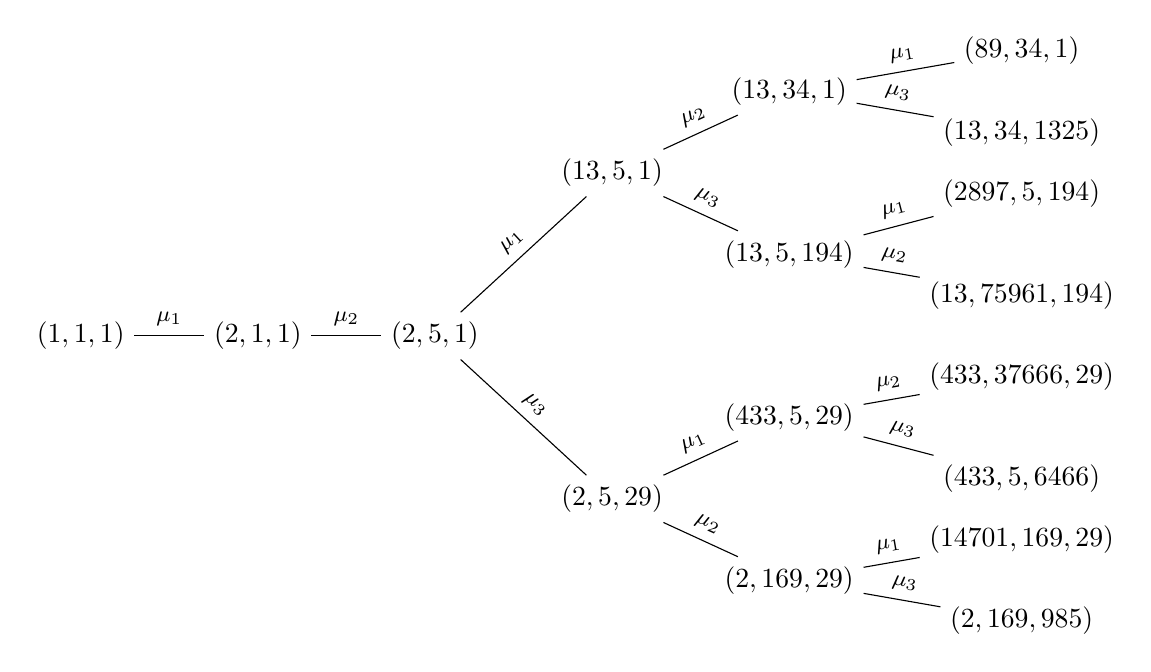
\begin{tikzpicture}[
				scale = 0.8,
				x = 5pt,
				y = 2.3pt,
				%  V/.style = ,
				every edge quotes/.style = {auto,sloped,font=\footnotesize} ]
			% \begin{scope}[nodes=V]
			\node (0) at (0,0)  {$(1,1,1)$};
			\node (1) at (16,0)    {$(2,1,1)$};
			\node (12) at (32,0)          {$(2,5,1)$};
			%
			\node (121) at (48, 32)    {$(13,5,1)$};
			\node (1212)  at (64, 48) {$(13,34,1)$};
			\node (12121) at (85, 56) {$(89,34,1)$};
			\node (12123) at (85, 40) {$(13,34,1325)$};
			\node (1213)  at (64, 16) {$(13,5,194)$};
			\node (12131) at (85, 28) {$(2897,5,194)$};
			\node (12132) at (85, 8) {$(13,75961,194)$};
			%
			\node (123) at (48, -32)    {$(2,5,29)$};
			\node (1232)  at (64, -48) {$(2,169,29)$};
			\node (12323) at (85, -56) {$(2,169,985)$};
			\node (12321) at (85, -40) {$(14701,169,29)$};
			\node (1231)  at (64, -16) {$(433,5,29)$};
			\node (12313) at (85, -28) {$(433,5,6466)$};
			\node (12312) at (85, -8) {$(433,37666,29)$};
			% \end{scope}
			\draw   (0)  edge["$\mu_1$"] (1)
			(1)  edge["$\mu_2$"] (12)
			%
			(12)  edge["$\mu_1$"] (121)
			(121)  edge["$\mu_2$"] (1212)
			(1212)  edge["$\mu_1$"] (12121)
			(1212)  edge["$\mu_3$"] (12123)
			(121)  edge["$\mu_3$"] (1213)
			(1213)  edge["$\mu_1$"] (12131)
			(1213)  edge["$\mu_2$"] (12132)
			%
			(12)  edge["$\mu_3$"] (123)
			(123)  edge["$\mu_2$"] (1232)
			(1232)  edge["$\mu_1$"] (12321)
			(1232)  edge["$\mu_3$"] (12323)
			(123)  edge["$\mu_1$"] (1231)
			(1231)  edge["$\mu_3$"] (12313)
			(1231)  edge["$\mu_2$"] (12312)
			;
		\end{tikzpicture}

		\caption{A part of the exchange graph of the Markov quiver, where the nodes are labeled by the corresponding Markov triplet.}
		\label{fig:markov_exchange_graph}
	\end{figure}
\end{example}

\begin{example}

	The recurrence relation \cref{eq:somos_4}, defining the Somos-4 sequence\index{Somos-4
		sequence} can also be recovered from the seed mutations corresponding to a certain
	quiver. Namely, consider the seed
	\begin{equation*}
		Q =
		\begin{tikzcd}[sep=large]
			1 \drar[shift left] \drar[shift right] & 2 \lar \dlar[shift left] \dlar[shift right] \\
			4 \uar \rar & 3 \uar[shift left] \uar \uar[shift right]
		\end{tikzcd}
		,\quad
		\bx = \{ x_1, x_2, x_3, x_4\}
	\end{equation*}
	%
	Mutating at the first vertex gives the seed
	\begin{equation*}
		\mu_1(Q) =
		\begin{tikzcd}[sep=large]
			1 \dar \rar & 2 \dlar[shift left] \dlar[shift right]  \\
			4 \rar[shift left] \rar[shift right] \rar & 3 \uar \ular[shift left] \ular[shift right]
		\end{tikzcd}
		,\quad
		\mu_1(\bx) = \left\{ \frac{x_2 x_4 + x_3^2}{x_1}, x_2, x_3, x_4\right\}
	\end{equation*}
	%
	We now note that $\mu_1(Q)$ is given by relabeling the vertices of $Q$ via $1 \mapsto
		2, 2 \mapsto 3, 3 \mapsto 4, 4\mapsto 1$, and that $\mu_1(x_1)$ is given by the same
	formula as \cref{eq:somos_4}. Thus, by mutating consecutively at the vertices
	$1,2,3,4,1,2,3,4,\dots$ the new cluster variables will correspond to the terms in the
	Somos-4 sequence. The Laurent phenomenon now guarantees that the sequence consists of
	integers when we set $a_0 = a_1 = a_2 = a_3 = 1$, as the denominators of all the terms
	will be monomials in $a_0, a_1, a_2$ and $a_3$.
\end{example}

\begin{example}

	We already gave an idea of how the Laurent phenomenon can be used to construct frieze
	patterns in \cref{exmp:frieze_patterns}\index{frieze pattern}. We can now make this
	more precise. Namely, to make a frieze pattern with $n$ rows (excluding the bounding
	rows of ones and zeros), one should consider the $A_n$ quiver (cf.
	\cref{fig:dynkin_diagrams_ade}). It will be easiest to explain this with an example.
	Consider again the frieze pattern:
	\begin{equation*}
		\dots\quad
		\begin{tikzcd}[
				sep = 0.2em, cramped,
			]
			1&&1&&1&&1&&1&&1&&1&&1&&1&&1&&1\\
			&1&&2&&2&&3&&1&&2&&4&&1&&2&&2&&3\\
			3&&1&&3&&5&&2&&1&&7&&3&&1&&3&&5\\
			&2&&1&&7&&3&&1&&3&&5&&2&&1&&7&&3\\
			3&&1&&2&&4&&1&&2&&2&&3&&1&&2&&4\\
			&1&&1&&1&&1&&1&&1&&1&&1&&1&&1&&1
		\end{tikzcd}
		\quad
		\dots
	\end{equation*}
	%
	In this case we need (an orientation of) the $A_4$ quiver. We can choose any lattice
	path from top to bottom. Then, the edges are oriented so that they always point from
	left to right.
	\begin{equation*}
		\dots\quad
		\begin{tikzcd}[
				sep = 0.2em, cramped,
			]
			1&&1&&1&&1&&1&&1&&1&&1&&1&&1&&1\\
			&1&&2&&2\drar[shorten=-0.15em] &&3&&1&&2&&4&&1&&2&&2&&3\\
			3&&1&&3&&5 \drar[shorten=-0.15em] &&2&&1&&7&&3&&1&&3&&5\\
			&2&&1&&7&&3&&1&&3&&5&&2&&1&&7&&3\\
			3&&1&&2&&4\urar[shorten=-0.15em] &&1&&2&&2&&3&&1&&2&&4\\
			&1&&1&&1&&1&&1&&1&&1&&1&&1&&1&&1
		\end{tikzcd}
		\quad
		\dots
	\end{equation*}
	%
	Mutating at a sink or a source, only changes the orientation of the edges, and does not
	introduce new edges. For example, mutation at a sink gives
	\begin{equation*}
		\begin{tikzcd}
			\cdots b \rar &d & \lar c \cdots & \, \rar[rightsquigarrow, "\mu_d"] & \,&
			\cdots  b & \lar \rar d & c \cdots
		\end{tikzcd}
	\end{equation*}
	%
	The mutated cluster variable corresponding to $d$ is then given by $d' = \frac{bc +
			1}{d}$. If we call this $a$, then find that $ad - bc = 1$, which is precisely the
	$\SL_2(\bbZ)$ diamond rule. Similarly, mutation at a source would compute $d$ in terms
	of $a$ in the $\SL_2(\bbZ)$ diamond. In the example, mutation at the vertex labeled 3
	results in changing the lattice path from $2 \to 5 \to 3 \gets 4$ to $2 \to 5 \gets 7
		\to 4$. Applying the Laurent phenomenon now shows that all the entries in the frieze
	pattern are Laurent polynomials in the entries of the initial lattice path. In
	particular, if one starts with a lattice path consisting of only ones, then all the
	entries will be integers. Do note that there exist frieze patterns which do not have a
	lattice path from top to bottom consisting of only ones:
	\begin{equation*}
		\begin{tikzcd}[sep=0.2em,cramped]
			1&&1&&1&&1&&1&&1&&1&&1&&1&&1&&1\\
			&1&&2&&4&&1&&2&&4&&1&&2&&4&&1&&2\\
			3&&1&&7&&3&&1&&7&&3&&1&&7&&3&&1\\
			&2&&3&&5&&2&&3&&5&&2&&3&&5&&2&&3\\
			3&&5&&2&&3&&5&&2&&3&&5&&2&&3&&5\\
			&7&&3&&1&&7&&3&&1&&7&&3&&1&&7&&3\\
			2&&4&&1&&2&&4&&1&&2&&4&&1&&2&&4\\
			&1&&1&&1&&1&&1&&1&&1&&1&&1&&1&&1
		\end{tikzcd}
	\end{equation*}

	The periodicity of the frieze patterns can also be explained through cluster algebras.
	It follows in part from \cref{thm:cluster_finite_classification}. A more precise
	conclusion about the periodicity can be obtained using more advanced results. For
	example, \cite[Theorem 8.8]{FominZelevinsky2007CA4Coefficients} gives that the period
	divides $2(n + 1 + 2) = 2n +6$. Indeed, in the frieze pattern of
	\cref{exmp:frieze_patterns} we had observed a period of $7$ which is exactly half of
	$2\cdot 4 + 6 = 14$. For a more detailed overview of the connections between cluster
	algebras and frieze patterns, we refer the reader to the survey paper
	\cite{BaurFaberGratz2018ConwayCoxeterFriezes}.
\end{example}

For \cref{exmp:triangulations} it will be more convenient to use a more general
definition of a cluster algebra. Namely, that of a cluster algebra with coefficients.

\section{Ice quivers and coefficients}\label{sec:ice_quivers_and_coefficients}

In the previous section we looked at cluster algebras coming from quivers. These are in
some sense the simplest kind of cluster algebras. In some cases, a more general notion
is needed. For example \cref{exmp:triangulations} will involve quivers with certain
vertices being frozen. When looking at quantum cluster algebras, we will need
skew-symmetrizable cluster algebras. All of these will be looked at in this section. To
avoid confusion, we will be very precise in this chapter with the names and
definitions. In the notation of this section, the cluster algebras coming from quivers
that we saw in the previous chapter would be referred to as a \emph{skew-symmetric
	cluster algebras of geometric type without coefficients}. Along the way, we will remove
more and more adjectives until we are just left with the definition of a cluster
algebra.

\subsection{Ice quivers}

Recall that in \cref{exmp:triangulations}, the length of a diagonal was obtained using
Ptolomy's theorem. The calculation involves the lengths of some of the diagonals, as
well as the lengths of some of the sides. Thus, the cluster variables should be
associated with both the diagonals as well as the sides. This poses a slight problem.
It is not possible to perform a flip on one of the sides of the $n$-gon. To fix this,
we will make a distinction between \emph{exchangeable} and \emph{frozen} vertices. This
leads to the notion of an \emph{ice quiver}\index{quiver!ice}.

Fix a subset $\ex \subseteq [1, N]$. The elements of $\ex$ will be called
\emph{exchangeable}\index{exchangeable}, while the elements of $\frz = [1, N] \setminus
	\ex$ will be called \emph{frozen}\index{frozen}. An \emph{ice quiver}, $\tQ$, is then
just the same as a normal quiver, except that we distinguish between the frozen and
exchangeable vertices. Although not strictly necessary, we will assume that the quiver
$\tQ$ contains no arrows between the frozen vertices, i.e., the vertices in $\tQ_0 \cap
	\frz$. Arrows between exchangeable and frozen vertices are allowed. When drawing a
quiver, the frozen vertices will be drawn with a box, while the exchangeable vertices
will just be drawn normally. The subquiver spanned by the exchangeable vertices, will
be called the \emph{principal part}\index{quiver!principal part of} of $\tQ$, and
denoted with just $Q$.

The definition of a seed remains very similar in this context. The naming will become
clear later.
\begin{definition}

	A \emph{skew-symmetric labeled seed of geometric type}\index{seed!skew-symmetric of
		geometric type} is a tuple $(\tQ, \tbx)$, where $\tQ$ is an ice quiver, and $\tbx =
		\{x_1, \dots, x_N\}$ is a free generating set of $\mcF$. The set $\tbx$ will be
	referred to as the \emph{extended cluster}\index{cluster!extended}, while the set $\bx
		= \{x_i \in \tbx \mid i \in \ex\}$ will be called the \emph{cluster}. The elements of
	$\bx$ will be called \emph{cluster variables}\index{cluster!variable}, while the
	elements of $\tbx \setminus \bx$ will be called \emph{frozen variables}.
\end{definition}

A seed such as in the previous section will be referred to as a \emph{skew-symmetric
	labeled seed of geometric type without coefficients}. It corresponds to the special
case where $\frz = \emptyset$. In the literature, the suffix ``with coefficients'' is
sometimes appended to indicate that $\frz \neq \emptyset$.

Seed mutation is now defined analogously, except that mutation can only be done at the
exchangeable indices, and that potential new arrows between frozen vertices in the ice
quiver are discarded. We then obtain the following definition.
\begin{definition}

	Let $\binv \subseteq \frz$ be any subset and $(\tQ, \tbx)$ be a skew-symmetric labeled
	seed of geometric type. Write $R = \bbK[x_i, x_j^{\pm 1} \mid i \in \frz \setminus
		\binv,\, j \in \binv]$. Then the \emph{skew-symmetric cluster algebra of geometric
		type}\index{skew-symmetric!cluster algebra of geometric type}, $\mcA(\tQ, \tbx,
		\binv)$\index{A Qt xt inv@$\mcA(\tQ, \tbx, \binv)$} is the $R$-subalgebra of $\mcF$
	generated by all the cluster variables of all the clusters of seeds mutation-equivalent
	to $(\tQ, \tbx)$.
\end{definition}

The main theorems from the previous section carry over with some small modifications.
\begin{theorem}

	Let $\mcA(\tQ, \tbx, \binv)$ be a skew-symmetric cluster algebra of geometric type.
	\begin{itemize}
		\item It is cluster-finite if and only if the ice quiver $\tQ$ is mutation-equivalent to an
		      ice quiver such that the connected components of its principal part are simply-laced
		      Dynkin diagrams \cite{FominZelevinsky2003CAFin}.
		\item It is mutation-finite if and only if it is either cluster-finite, obtained from a
		      surface or is one of a few exceptions \cite{FeliksonPavel2023cluster}.
		\item The Laurent phenomenon holds. More precisely, let $(\tQ', \tbx')$ be any seed
		      mutation-equivalent to $(\tQ, \tbx)$, and $x$ any cluster variable of this seed. Then
		      $x$ is a Laurent polynomial with integer coefficients in the extended cluster variables
		      of the initial seed \cite{FominZelevinsky2002CAF}. The frozen variables do not appear
		      as denominators in the Laurent polynomials, i.e., $x \in \bbZ[x_i^{\pm 1}, x_j \mid i
			      \in \ex,\, j \in \frz]$ \cite[Theorem 3.3.6]{FominWilliams2021IntroductionCA_1-3}.
		\item The integer coefficients can be taken to be positive
		      (\cite{LeeSchiffler2015PositivityCA}).
	\end{itemize}
\end{theorem}

\textbf{TODO: triangulations example revisited.}

\subsection{Skew-symmetrizable matrices}

Thusfar, all the cluster algebras have been constructed from (ice) quivers.
Equivalently, one can work with matrices, as we know explain.

Let $\tQ$ be an ice quiver with exchangeable vertices labeled by $\ex$ and frozen
vertices labeled by $\frz$. Associated to $\tQ$ is an $N \times |\ex|$ integer matrix
$(b_{ik}) = \tB \in M_{N \times \ex}(\bbZ)$. The notation indicates that the columns
are indexed by $\ex$ instead of $[1, |\ex|]$. The elements are given by
\begin{equation*}
	b_{ik} = \begin{dcases*}
		|\{ i \to k\}|, & if $\{i \to k\} \neq \emptyset$ \\
		-|\{k \to i\}|, & if $\{k \to i\} \neq \emptyset$ \\
		0,              & otherwise,
	\end{dcases*}
\end{equation*}
%
for $i \in [1, N]$ and $k \in \ex$. It is not a square matrix because we assume that
there are no arrows between frozen vertices. The $|\ex| \times |\ex|$ submatrix $B \in
	M_{\ex \times \ex}(\bbZ)$ of $\tB$ given by the rows in $\ex$ will be called the
\emph{principal part}\index{principal part} of $\tB$. Note that the principal part of
$\tB$ is \emph{skew-symmetric}\index{skew-symmetric}\index{matrix!skew-symmetric},
i.e., $b_{ik} = - b_{ki}$ for all $i,k \in \ex$ or equivalently $B^T = - B$.

Conversely, starting from a matrix $\tB \in M_{N \times \ex}(\bbZ)$ whose principal
part is skew-symmetric, one can associate an ice quiver $\tQ$, by placing $b_{ik}$
arrows from the vertex $i$ to the vertex $k$, for each $i \in [1, N]$ and $k \in \ex$.

\begin{example}
	Consider the ice quiver
	\begin{equation*}
		Q = \begin{tikzcd}[sep=scriptsize]
			\boxed{1} \\
			2 \uar \rar[shift left]\rar[shift right] & 3  \rar \dar & 4 \\
			& \boxed{5} \ular
		\end{tikzcd},
	\end{equation*}
	%
	where $\ex = \{2,3,4\}$. The associated matrix $\tB \in M_{5 \times \ex}$ and principal
	part $B \in M_{\ex \times \ex}$ are given by
	\begin{equation*}
		\tB =
		\begin{pmatrix}
			-1 & 0  & 0 \\
			0  & 2  & 0 \\
			-2 & 0  & 1 \\
			0  & -1 & 0 \\
			1  & -1 & 0
		\end{pmatrix}
		,\quad B =
		\begin{pmatrix}
			0  & 2  & 0 \\
			-2 & 0  & 1 \\
			0  & -1 & 0
		\end{pmatrix}.
	\end{equation*}
\end{example}

Let $\tQ$ be an ice quiver with associated matrix $\tB$. We now want to describe what
happens to the matrix $\tB$ after mutation. Take some $k \in \ex$, and denote the
elements of $\mu_k(\tB)$ with $b'_{ij}$.
\begin{enumerate}
	\item The vertices of $\tQ$ remain unchanged under mutation. Thus, $\mu_k(\tB) \in M_{N
				      \times \ex}(\bbZ)$.
	\item For $i \in [1, N]$ and $j \in \ex$, we need to create a new arrow $i \to j$ for each
	      path $i \to k \to j$. There is a path $i \to k \to j$ if and only if $b_{ik} >0$ and
	      $b_{kj} > 0$. The number of paths $i\to j\to k$ is then given by $b_{ik}b_{kj}$.
	      Conversely, we need to create an arrow $j \to i$ for each path $j \to k \to i$. Such
	      paths exist if $b_{ik} <0$ and $b_{kj} < 0$. In this case, the number of paths is also
	      given by $b_{ik}b_{kj}$.
	\item Finally, for $i \in [1,N]$, we need to flip the orientation of all the arrows $i \to k$
	      or $k \to i$. This translates to setting $b'_{ij} = -b_{ij}$ for all $i \in [1, N]$ and
	      $j \in \ex$ such that $i = k$ or $j = k$.
\end{enumerate}
As a result we derive the following mutation rule for the mutation in direction $k\in \ex$:
\begin{equation}\label{eq:mutation_rule_matrix_expanded}
	b'_{ij} \defeq \begin{dcases*}
		-b_{ij},               & if $i = k$ or $j = k$  \\
		b_{ij} + b_{ik}b_{kj}, & if $b_{ik},b_{kj} > 0$ \\
		b_{ij} - b_{ik}b_{kj}, & if $b_{ik},b_{kj} < 0$ \\
		b_{ij},                & otherwise,
	\end{dcases*}
	\quad \text{for } i \in [1, N],\,j \in \ex.
\end{equation}
%
This can be further condensed into the following rule.
\begin{equation}\label{eq:mutation_rule_matrix_condensed}
	b'_{ij} \defeq \begin{dcases*}
		-b_{ij},                                            & if $i = k$ or $j = k$ \\
		b_{ij} + \frac{|b_{ik}|b_{kj} + b_{ik}|b_{kj}|}{2}, & otherwise.
	\end{dcases*}
\end{equation}

To express the exchange relation in terms of the matrix $\tB$ we first introduce some
notation. Write $[b_{ij}]_{+} = \max\{b_{ij}, 0\}$ and $[b_{ij}]_{-} \defeq
	\min\{b_{ij}, 0\}$. Then the exchange rule \cref{eq:exchange_relation_quiver}
translates into
\begin{equation}\label{eq:exchange_relation_matrix}
	x'_k = \frac{1}{x_k}\left(\prod_{i=1}^n x_i^{[b_{ik}]_{+}} + \prod_{i=1}^{N} x_i^{-[b_{ik}]_{-}}\right).
\end{equation}

Because working with the matrix $\tB$ is equivalent to working with the ice quiver
$\tQ$, we will use the same name for the corresponding seeds and cluster algebras.
\begin{definition}

	A \emph{skew-symmetric labeled seed of geometric type}\index{seed!skew-symmetric of
		geometric type} if a tuple $(\tB, \tbx)$, where $\tB \in M_{N \times \ex}(\bbZ)$ has
	skew-symmetric principal part, and $\tbx = \{x_1, \dots, x_N\}$ is a free generating
	set of $\mcF$. The mutation of the seed $(\tB, \tbx)$ in direction $k \in \ex$ is given
	by the seed $(\mu_k(\tB), \mu_k(\tbx))$ where $\mu_k(\tB)$ is given by
	\cref{eq:mutation_rule_matrix_condensed} and $\mu_k(\tbx)$ is given by $\{x_1', \dots,
		x_N'\}$ where $x_i' = x_i$ for $i\neq k$ and $x'_k$ is given by
	\cref{eq:exchange_relation_matrix}. The \emph{skew-symmetric cluster algebra of
		geometric type}\index{skew-symmetric!cluster algebra of geometric type}, $\mcA(\tB,
		\ex, \binv)$\index{A Bt xt inv@$\mcA(\tB, \tbx, \binv)$} is then defined completely
	analogously to the version with ice quivers.
\end{definition}

Interestingly, note that for \emph{any} matrix $\tB \in M_{N\times \ex}(\bbZ)$, the
mutation rule \cref{eq:mutation_rule_matrix_expanded}, defines an involution. Indeed,
if $i = k$ or $j = k$ then $b''_{ij} = -b'_{ij} = b_{ij}$. Otherwise, if $b_{ik} > 0$
and $b_{kj} >0$, then $b'_{ik} = -b_{ik} < 0$ and $b'_{kj} = -b_{kj} < 0$ so that
\begin{equation*}
	b''_{ij} = b'_{ij} - b'_{ik}b'_{kj} = b_{ij} + b_{ik}b_{kj} - b_{ik}b_{kj} = b_{ij}.
\end{equation*}
%
Similarly, if $b_{ik} < 0$ and $b_{kj} < 0$. In the other cases mutation does not
change $b_{ij}$.

Additionally, remark that if $B$ is the principal part of $\tB$, then the principal
part of $\mu_k(\tB)$ is given by $\mu_k(B)$. Thus, the mutation of $B$ does not depend
on the entries of $\tB$ which are not contained in $B$.

One might wonder if we can simply drop the skew-symmetric condition on the principal
part of $\tB$ all together. It turns out that in order to have a nice enough ``exchange
pattern'', the minimal requirement is that the principal part of $\tB$ and all matrices
mutation-equivalent to it should be \emph{sign-
	skew-symmetric}\index{skew-symmetric!sign-}\index{matrix!sign-skew-symmetric}
(\cite[Proposition 4.3]{FominZelevinsky2002CAF}). A matrix $B \in M_N(\bbZ)$ is said to
be sign-skew-symmetric if for all $i,j \in [1, N]$, the entries $b_{ij}$ and $b_{ji}$
are both zero, or have opposite signs. In particular, skew-symmetric matrices are sign
skew-symmetric. The problem is that mutation of a sign-skew-symmetric matrix might
yield a matrix which is no longer sign-skew-symmetric.

\begin{example}
	Consider the sign-skew-symmetric matrix
	\begin{equation*}
		C = \begin{pmatrix}
			0  & 1  & -1 \\
			-2 & 0  & 4  \\
			3  & -1 & 0
		\end{pmatrix}.
	\end{equation*}
	%
	Mutation in direction $1$ using \cref{eq:mutation_rule_matrix_expanded} gives the
	matrix
	\begin{equation*}
		\mu_1(C) = \begin{pmatrix}
			0  & -1 & 1 \\
			2  & 0  & 2 \\
			-3 & 2  & 0
		\end{pmatrix},
	\end{equation*}
	which is no longer sign-skew-symmetric.
\end{example}

There is a class of matrices between sign-skew-symmetric matrices and skew-symmetric
matrices. These are the \emph{skew-symmetrizable
	matrices}\index{matrix!skew-symmetrizable}. A matrix $B \in M_N(\bbZ)$ is said to be
skew-symmetrizable if there exist $d_1, \dots, d_N \in \bbZ_{\geq 0}$ such that
\begin{equation}\label{eq:skew_symmetrizable}
	d_i b_{ij} = -d_j b_{ji}\quad  \text{ for all } i,j \in [1, N].
\end{equation}
%
We say that $B$ is skew-symmetrizable by the integers $d_1, \dots, d_N$. Write $D \in
	M_N{\bbZ}$ for the diagonal matrix with the elements $d_1, \dots, d_N$ on the diagonal.
Then \cref{eq:skew_symmetrizable} translates to $(DB)^T = -DB$, i.e., the matrix $DB$
is skew-symmetric.

\begin{proposition}\label{prop:mutation_preserves_skew_symmetrizable}
	Suppose that $B \in M_N(\bbZ)$ is skew-symmetrizable by the positive integers $d_1, \dots, d_N \in \bbZ_{>0}$. Then $B$ is sign-skew-symmetric, and for any $k \in [1, N]$, the matrix $\mu_k(B)$ is sign-skew-symmetric and skew-symmetrizable by the same integers.
\end{proposition}
\begin{proof}
	Since the integers $d_1, \dots, d_N$ are strictly positive, \cref{eq:skew_symmetrizable} implies that $B$ is sign-skew-symmetric. Furthermore, for $i,j \in [1, N]$ we have
	\begin{equation*}
		d_i b'_{ij} = - d_i  b_{ij} = d_j b_{ji} = -d_j b'_{ji}
	\end{equation*}
	if $i =k$ or $j = k$, and
	\begin{align*}
		d_i b'_{ij}
		 & = d_i b_{ij} + \frac{|d_i b_{ik}|b_{kj} + d_i b_{ik}|b_{kj}|}{2}         \\
		 & = - d_j b_{ji} + \frac{|d_k b_{ki}|b_{kj} - d_k b_{ki}|b_{kj}|}{2}       \\
		 & = - d_j b_{ji} + \frac{ - |b_{ki}| d_j b_{jk} - b_{ki}|d_jb_{jk}|}{2}    \\
		 & = - d_j\left( b_{ji} + \frac{|b_{jk}|b_{ki} +  b_{jk}|b_{ki}|}{2}\right) \\
		 & = - d_jb'_{ji},
	\end{align*}
	otherwise.
\end{proof}

It is now a natural question to ask whether all sign-skew-symmetric matrices which
remain sign-skew-symmetric under mutations are skew-symmetrizable. This turns out not
to be the case. For example, for $\alpha, \beta, \gamma \in \bbZ_{>0}$ such that
$\alpha\beta\gamma \geq 0$, the matrix
\begin{equation*}
	\begin{pmatrix}
		0             & 2\alpha         & -2\alpha \beta \\
		-\beta \gamma & 0               & 2 \beta        \\
		\gamma        & - \alpha \gamma & 0
	\end{pmatrix}
\end{equation*}
%
is sign-skew-symmetric, not skew-symmetrizable, and it remains sign-skew-symmetric
under any sequence of mutations (\cite[Proposition 4.7]{FominZelevinsky2002CAF}). In
practice, however, one always restricts to the skew-symmetric or skew-symmetrizable
case.
\begin{definition}

	A pair $(\tB, \tbx)$, where $\tB \in M_{N \times \ex}(\bbZ)$ is such that its principal
	part is skew-symmetrizable and $\tbx = \{x_1, \dots, x_N\}$ is a free generating set of
	$\mcF$ is called a \emph{labeled seed of geometric type}\index{seed!of geometric type}.
	Seed mutation and the corresponding \emph{cluster algebra of geometric
		type}\index{cluster algebra!of geometric type} are defined completely analogously as in
	the case of skew-symmetric seeds of geometric type.
\end{definition}

The main results from the skew-symmetric case also hold in the skew-symmetrizable case.
The cluster-finite classification now encompasses all the Dynkin diagrams. We refer the
reader to \cite[Chapter 5]{FominWilliams2021IntroductionCA_4-5} for a good overview of
Cartan matrices, Dynkin diagrams and the classification.
\begin{theorem}[\protect{\cite[Theorem 1.4]{FominZelevinsky2003CAFin}}]

	Let $\mcA(\tB, \tbx, \binv)$ be a cluster algebra of geometric type. Write $A(B) \in
		M_{\ex \times \ex}(\bbZ)$ for the matrix with entries
	\begin{equation*}
		(a_{ij}) = \begin{dcases*}
			2,         & if $i = j$     \\
			-|b_{ij}|, & if $i \neq j$.
		\end{dcases*}
	\end{equation*}
	%
	Then $\mcA(\tB, \tbx, \binv)$ is cluster-finite if and only if $A(B)$ is a \emph{Cartan
		matrix of finite type}\index{matrix!Cartan}, i.e., $a_{ij}a_{ji} \leq 3$ for all $i
		\neq j$.
\end{theorem}

The mutation-finite classification remains roughly the same. One has to replace quivers
by \emph{diagrams}\index{diagram} and surfaces by \emph{orbifolds}\index{orbifold}
(\cite{FeliksonPavel2023cluster}). Since we will not need this result, we refrain from
giving the relevant definitions.

Finally, the Laurent phenomenon and positivity still hold without any changes. Proving
positivity in this setting took a long time, and required advanced methods. It was
shown along with some other open conjectures at the time in a groundbreaking paper by
Gross, Hacking, Keel and Kontsevich
(\cite{GrossHackingKeelKontsevich2018CanonicalBCA}).

\textbf{TODO: rank 2 cluster algebras example}

\subsection{Cluster algebras with coefficients}\label{sec:cluster_algebras_coefficients}

We now finally tackle the most generally notion of a cluster algebra. After giving the
relevant definitions, we will explain how the previous definitions are special cases,
and justify the terminology used. Finally we will give an overview of the various
definitions and the important theorems.

\textbf{TODO: coefficients}

\section{Cluster algebras from surfaces}\label{sec:cluster_algebras_surfaces}

\subsection{The Grassmannian}

Definition of Grassmannian. Plucker coordinates, algebra relations. Special case of
$k=2$. Correspondence with triangulations.
\subsection{Marked surfaces with punctures}\label{sec:triangulations_of_surfaces}
Explain how to generalize to marked surfaces with punctures.

% \begin{example}\label{exmp:markov_upper_via_triangulation}
% 	\textbf{TODO: markov cluster algebra not upper cluster algebra: see https://www.math.uni-bonn.de/people/sefil/Papers/punct.pdf}
% \end{example}
\subsection{Examples}


\newcommand{\bbr}{\mathbf{r}}
\newcommand{\bbn}{\boldsymbol{\nu}}
\newcommand{\bbl}{\boldsymbol{\lambda}}
\newcommand{\bbg}{\boldsymbol{\gamma}}
\newcommand{\oy}{\overline{y}}
\renewcommand{\oe}{\overline{e}}

\chapter{Quantum cluster algebras}
\section{Quantum tori}

Some of the basic background needed on quantum tori, and rational actions.

\section{Quantum cluster algebras}

Toric frames, quantum seeds and mutations. Quantum Laurent phenomenon.

\textbf{TODO: fill out these stubs}

\begin{lemma}\label{lem:principal_part_skew_symmetrizable}
	GY Lemma 2.4
\end{lemma}
\begin{proposition}\label{prop:mutation_preserves_good_things}
	GY Proposition 2.6
\end{proposition}
\begin{corollary}\label{cor:formula_for_mutation}
	GY Corollary 2.11
\end{corollary}
\begin{lemma}\label{lem:equivariance_mutations}
	GY Lemma 2.13
\end{lemma}

\section{Quantum Grassmannians}
???

\section{CGL extensions}

\textbf{Motivate section as a generic way to produce quantum cluster algebras.}

In this section we will look at a purely algebraic method of placing a quantum cluster
algebra structure on certain class of algebras as first presented in
\cite{GoodearlYakimov2017QCA}. Not only do these have the structure of a quantum
cluster algebra, they also equal the corresponding upper cluster algebra. Along the way
we will provide plenty of examples, to make it clear how the results can be applied in
practice.

\textbf{What is Ore extension. Example of Weyl algebra.}
\begin{definition}
	Let $R$ be a ring with unit, $\sigma \colon R \to R$ a ring endomorphism and
	$\delta \colon R \to R$ a $\sigma$-\emph{derivation}\index{ring!-derivation}, i.e.,
	$\delta$ is a group homomorphism $(R, +) \to (R, +)$ such that $\delta (r s) =
		\sigma(r)\delta(s) + \delta(r) s$. Then we write $R[x;\sigma, \delta]$ for the ring generated by $R$ and $x$ with the additional relation that
	\begin{equation*}
		x r = \sigma(r) x + \delta(r)
	\end{equation*}
	%
	for all $r \in R$. We call $R[x;\sigma, \delta]$ an \emph{Ore extension}\index{Ore
		extension} or \emph{skew polynomial ring}\index{ring!skew polynomial}. The conditions
	on $\sigma$ and $\delta$ ensure that the multiplication is well-defined.
\end{definition}
%
\begin{convention}
	%
	In what follows, when $R[x;\sigma, \delta]$ is an Ore extension, $R$ is a
	$\bbK$-algebra, $\sigma$ is a $\bbK$-algebra \emph{automorphism} and $\delta$ is a
	$\bbK$-linear $\sigma$-derivation. In this case, $R[x;\sigma, \delta]$ is also a
	$\bbK$-algebra.
\end{convention}
%
Under these assumptions, the Ore extension $R[x; \sigma, \delta]$ is Noetherian when
$R$ is Noetherian. It will also be a domain if $R$ is a domain.

\begin{example}
	Let $A_1$ be the $\bbK$-algebra generated by two variables $x$ and $y$ such that $yx =
		xy + 1$. This algebra is known as the \emph{Weyl algebra}\index{algebra!Weyl}. It can
	also be viewed as an Ore extension $\bbK[x][y; \id, \partial_x]$:
	\begin{itemize}
		\item The base algebra is the polynomial ring $\bbK[x]$.
		\item The algebra endomorphism $\sigma$ is the identity.
		\item The $\sigma$-derivation $\delta$ is the formal derivative with respect to $x$:
		      \begin{equation*}
			      \partial_x \left(\sum_{i=0}^n a_i x^i \right) = \sum_{i=1}^{n} a_i i x^{i-1}.
		      \end{equation*}
		      %
		      That $\partial_x$ is a derivation follows from the ordinary product rule for derivatives.
	\end{itemize}
\end{example}

\textbf{What is rational action of a torus.}

We borrow some definitions from \cite{GoodearlBrown2002LecturesAQC}. Let $\mcH$ be a
group, and $A$ a $\bbK$-algebra. We say that $\mcH$ \emph{acts on $A$ by
	automorphisms}\index{action!by automorphisms} if for every $h \in \mcH$, the map $A \to
	A \colon x \mapsto h \cdot x$ is a $\bbK$-algebra automorphism. A nonzero element $u
	\in A$ is called an \emph{$\mcH$-eigenvector}\index{H@$\mcH$!-eigenvector} if $\mcH
	\cdot u \subseteq \bbK u$. So, for each $h \in \mcH$ there exists some $\lambda_h \in
	\bbK$ such that $h \cdot u = \lambda_h u$. Since $\mcH$ acts by automorphisms,
$\lambda_h \neq 0$ for all $h \in \mcH$. So, we get a group homomorphism $\chi_u \colon
	\mcH \to \bbK^\times$ given by $\chi_u(h) = \lambda_h$. We call $\chi_u$ the
\emph{$\mcH$-eigenvalue}\index{H@$\mcH$!-eigenvalue} of $u$. Associated to each
$\mcH$-eigenvalue is its \emph{$\mcH$-eigenspace}\index{H@$\mcH$!-eigenspace}
\begin{equation*}
	A_\chi = \{u \in A \mid h \cdot x = \chi(h)x \forall h \in \mcH \}.
\end{equation*}
%
Finally, we say that the action is \emph{semisimple}\index{action!semisimple} if $A$ is
the direct sum of its $\mcH$-eigenspaces.

Now, let $\mcH$ be a \emph{$\bbK$-torus}\index{torus}, that is, a group of the form
$(\bbK^\times)^r$. By identifying $\mcH$ with the affine variety $\{(x_1, \dots, x_r,
	y) \in \bbK^{r+1} | x_1 \dots x_r y = 1\}$, we can view it as an algebraic group.
Assume that $\mcH$ acts on a $\bbK$-algebra $A$ by $\bbK$-algebra automorphisms. Then
we say that the action of $\mcH$ on $A$ is \emph{rational}\index{action!rational} if it
is semisimple, and all the corresponding $\mcH$-eigenvalues are morphisms of affine
varieties.

Write
\begin{equation*}
	X(\mcH) = \{\chi \in \Hom(\mcH, \bbK^\times) \mid \chi \text{ is a morphism of algebraic varieties}\},
\end{equation*}
%
for the character group\index{group!character} of $\mcH$. Then a rational action is the
same as an $X(\mcH)$-grading\index{grading} of $A$. Indeed, if we have a rational
action on $A$, then we can write
\begin{equation*}
	A = \bigoplus_{\chi \in X(\mcH)} A_\chi,
\end{equation*}
which is graded because for $a \in A_\chi, b \in A_{\chi'}$ and all $h \in \mcH$:
\begin{align*}
	h \cdot (a b) = (h\cdot a)(h\cdot b)= \chi(h)a \chi'(h)b = (\chi \chi')(h)ab,
\end{align*}
so that $ab \in A_{\chi \chi'}$. Conversely, if
\begin{equation*}
	A = \bigoplus_{g \in X(\mcH)} A_g
\end{equation*}
is a grading, then we get a rational action through
\begin{equation*}
	h \cdot x = h \cdot \left(\sum_{g \in X(\mcH)} x_g \right) = \sum_{g \in X(\mcH)} g(h)x.
\end{equation*}
%
Under this correspondence, the $\mcH$-eigenvectors are precisely the nonzero
homogeneous\index{element!homogeneous} elements under the grading.

\textbf{TODO: Examples}.

\textbf{Def CGL extension. Example of matrices, and Heisenberg algebra.}

The combination of a rational action by a torus and iterated Ore extensions gives rise
to the following definition:
\begin{definition}[\protect{\cite[Definition 3.3]{GoodearlYakimov2017QCA}}]\label{def:cgl_extension}
	An iterated Ore extension
	\begin{equation*}
		R = \bbK[x_1][x_2; \sigma_2, \delta_2]\cdots [x_N; \sigma_N, \delta_N]
	\end{equation*}
	is called a \emph{CGL extension}\index{CGL extension} if it is equipped with a rational action of a $\bbK$-torus $\mcH$ by $\bbK$-algebra automorphisms such that
	\begin{enumerate}
		\item\label{itm:x_i-eigenvectors} The elements $x_1, \dots, x_N$ are $\mcH$-eigenvectors.
		\item For every $k\in [2, N]$, $\delta_k$ is \emph{locally
			      nilpotent}\index{nilpotent!locally}, i.e., for all $r \in R_{k-1}$, there exists some
		      $n \in \bbZ_{>0}$ such that $\delta_k^n (r) = 0$. Here, $R_{k-1}$ denotes the
		      intermediate algebra consisting of only the first $k-1$ extensions:
		      \begin{equation*}
			      R_{k-1} = \bbK[x_1][x_2; \sigma_2, \delta_2]\cdots[x_{k-1};\sigma_{k-1}, \delta_{k-1}].
		      \end{equation*}
		      %
		      \item\label{itm:sigma_k-is-h_k} For every $k \in [1, N]$, there exists $h_k \in \mcH$ such that $\sigma_k$ is given by the action of $h_k$ on $R_{k-1}$ and the $h_k$-eigenvalue of $x_k$, is not a root of unity.
	\end{enumerate}
\end{definition}

We will call $N$ the length\index{CGL extension!length of} of the CGL extension. As
mentioned in the definition, we denote by $R_k$ the intermediate subalgebra generated
by the first $k$ variables. For $j, k \in [1, N]$ we will also use the notation $R_{[j,
					k]}$ to denote the unital subalgebra generated by ${x_i \mid j \leq i \leq k}$ where
$R_{[j, k]} = \bbK$ if $j \nleq k$.

We will write $\lambda_k$ for the $h_k$-eigenvalue of $x_k$, i.e., $h_k \cdot x_k =
	\lambda_k$. For $1 \leq j < k \leq N$, we have $\sigma_k (x_j) = h_k \cdot x_j =
	\lambda_{kj} x_j$ for some $\lambda_{kj} \in \bbK^\times$ using conditions
\labelcref{itm:x_i-eigenvectors,itm:sigma_k-is-h_k}. We can complete this to a
multiplicatively skew-symmetric matrix
\begin{equation}\label{eq:CGL_lambda}
	\boldsymbol{\lambda}= (\lambda_{kj}) \in M_N(\bbK^\times)
\end{equation}
%
by setting $\lambda_{kk} = 1$ and $\lambda_{jk} = \lambda_{kj}\inv$ for $1 \leq j < k
	\leq N$.

\begin{lemma}\label{lem:h_after_delta}
	With the notations as in \cref{def:cgl_extension},
	\begin{equation*}
		(h\cdot )\delta_k = \chi_{x_k}(h)\delta_k(h\cdot),
	\end{equation*}
	for all $h \in \mcH$ and $k \in [2, N]$.
\end{lemma}
\begin{proof}
	Fix $k \in [2, N]$ and $h \in \mcH$. Note that any monomial $a = x_1^{m_1}\cdots x_{k-1}^{m_{k-1}} \in R_{k-1}$ is an $h$-eigenvector, and also a $\sigma_k$-eigenvector. Hence,
	\begin{align*}
		h \cdot(x_k a)  & = \chi_{x_k}(h)\chi_{a}(h)x_ka                                      \\
		                & = \chi_{x_k}(h)\chi_{a}(h)(\sigma_k (a)x_k +  \delta_k(a))          \\
		                & = h \cdot (\sigma_k (a) x_k) + \chi_{x_k}(h)\delta_k(\chi_{a}(h)a), \\
		\shortintertext{but also}
		h \cdot (x_k a) & = h \cdot (\sigma_k (a) x_k + \delta_k(a))                          \\
		                & = h \cdot (\sigma_k (a) x_k) + h\cdot \delta_k(a),
	\end{align*}
	which shows $h \cdot \delta_k (a) = \chi_{x_k}(h) \delta_k (h \cdot a)$. The result then follows from linearity of $(h \cdot)$ and $\delta_k$.
\end{proof}

For a given CGL extension, there is not necessarily a unique order in which the $x_1,
	\dots, x_N$ need to be added. The different permutations will correspond to cluster
algebra mutations. A symmetry condition ensures that the CGL extension has enough
presentations.

\begin{definition}[\protect{\cite[Definition 3.12]{GoodearlYakimov2017QCA}	}]
	We call a CGL extension, $R$, \emph{symmetric}\index{CGL extension!symmetric} if the following conditions hold
	\begin{enumerate}
		\item For all $1\leq j < k \leq N$,
		      \begin{equation*}
			      \delta_k (x_j) \in R_{[j+1, k-1]}.
		      \end{equation*}
		\item For all $j \in [1, N]$, there exists $h^*_j \in \mcH$ such that
		      \begin{equation*}
			      h^*_j \cdot x_k = \lambda_{kj}\inv x_k = \lambda_{jk}x_k, \, \forall k \in [j+1, N]
		      \end{equation*}
		      and $h^*_j \cdot x_j = \lambda^*_j x_j$ for some $\lambda_j^*\in \bbK^\times$ which is not a root of unity.
	\end{enumerate}
\end{definition}
For any symmetric CGL extension, we can make new CGL presentations as follows. Set
\begin{equation*}
	\sigma_j^* = (h_j^* \cdot) \in \End(R),\, \forall j \in [1, N-1].
\end{equation*}
Then, define the $\sigma_j^*$-derivation, $\delta_j^*$, of $R_[j+1, N]$ via
\begin{equation*}
	\delta_j^*(x_k) = x_j x_k - \lambda_{jk}x_kx_j = -\lambda_{jk} \delta_k (x_j), \, \forall k \in [j+1, N].
\end{equation*}
%
The conditions for $R$ to be a symmetric CGL extension then imply that $\sigma_k$ and
$\delta_k$ preserve $R_{[j, k-1]}$ and $\sigma_k^*, \delta_k^*$ preserve $R_{[j+1, k]}$
for all $1 \leq j < k \leq N$. This allows us to view $R_{[j, k]}$ in two ways:
\begin{equation*}
	R_{[j, k]} = R_{[j, k-1]}[x_k; \sigma_k, \delta_k] \text{ and } R_{[j,k]} = R_{[j+1, k]}[x_j; \sigma_j^*, \delta_j^*].
\end{equation*}
So, we can always extend the interval $[j, k]$ to the left or the right. Doing this recursively gives rise to an iterated Ore extension presentation for $R$. For example, starting with the variable $x_N$ and always extending the interval to the left, we obtain the presentation
\begin{equation*}
	R = \bbK[x_N][x_{N-1}; \sigma_{N-1}^*, \delta_{N-1}^*]\cdots [x_1, \sigma_1^*, \delta_1^*].
\end{equation*}
%
The types of permutations that we obtain this way consist of the following subset of
the symmetric group $S_N$:
\begin{equation*}
	\Xi_N = \{\tau \in S_N \mid \tau(k) = \max (\tau ([1, k-1])) + 1 \text{ or } \tau(k) = \min (\tau ([1, k-1])) - 1, \forall k \in [2, N]\}.
\end{equation*}
%
Each $\tau \in \Xi_N$ gives rise to a CGL presentation:
\begin{equation*}
	R = \bbK[x_{\tau(1)}][x_{\tau(2)}; \sigma_{\tau(2)}'', \delta_{\tau(2)}''] \cdots [x_{\tau(N)}; \sigma_{\tau(N)}'', \delta_{\tau(N)}''],
\end{equation*}
%
where $\sigma''_{\tau(k)} = \sigma_{\tau(k)}, \delta_{\tau(k)}'' = \delta_{\tau(k)}$
and $h_{\tau(k)}' = h_{\tau(k)}$ if $\tau(k) = \max(\tau([1,k-1])) + 1$, while
$\sigma''_{\tau(k)} = \sigma^*_{\tau(k)}, \delta_{\tau(k)}'' = \delta^*_{\tau(k)}$ and
$h_{\tau(k)}'' = h_{\tau(k)}^*$ if $\tau(k) = \min(\tau([1,k-1])) - 1$
(\cite[Proposition 3.14]{GoodearlYakimov2017QCA}).

\textbf{Homogeneous prime elements.}

A \emph{prime element}\index{element!prime} of a not necessarily commutative domain $R$
is a nonzero element $p \in R$ such that $p$ is \emph{normal}\index{element!normal},
that is, $Rp = pR$ and such that the quotient $R / Rp$ is a domain. To illustrate that
this definition corresponds to our intuition of what a prime element should be, we
prove the following small lemma.
\begin{lemma}\label{lem:prime_divides_product}
	%
	Let $p$ be a prime element in a ring $R$. If $p$ divides a product $ab$ for some $a,b
		\in R$, then $p$ divides $a$ or $p$ divides $b$.
\end{lemma}
\begin{proof}
	%
	Note that since $p$ is normal, there is no ambiguity about dividing $ab$ on the left or
	on the right. Indeed, if $c p = ab$ for some $c \in R$, then $ab \in Rp = pR$, and
	there exists some $c' \in R$ such that $p c' = ab$. So, assume that $ab \in Rp$. Then
	the image of $ab$ is zero under the quotient map $\pi \colon R \to R/Rp$. Since $Rp$ is
	a domain, that implies that either $\pi(a) = 0$ or $\pi(b)$ is zero. So, either $a \in
		Rp$ or $b \in Rp$.
\end{proof}
%
We now state a theorem that is quite technical, but forms the heart of the main
theorem. Let us first fix some notation. For a function $\eta \colon [1, N] \to \bbZ$,
we can define a predecessor and successor
function\index{function!predecessor}\index{function!successor}:
\begin{align*}
	p \colon [1, N] \to [1, N] \sqcup \{-\infty\} & \colon k \mapsto  \max\{j < k \mid \eta(j) = \eta(k)\}  \\
	s \colon [1, N] \to [1, N] \sqcup \{+\infty\} & \colon k \mapsto  \min\{j > k \mid \eta(j) = \eta(k)\},
\end{align*}
%
where we take $\max \{\} = - \infty$ and $\min \{\}= + \infty$ (cf.
\cref{fig:predecessor_successor}).

\begin{figure}
	\centering
	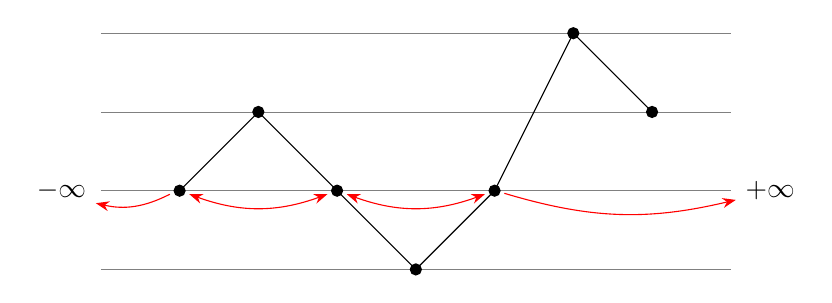
\begin{tikzpicture}
		\draw[help lines, xstep =0] (0,0) grid (8,3);
		\draw plot[mark=*] coordinates {(1,1) (2,2) (3,1) (4,0) (5,1) (6,3) (7,2)};
		\node (neginf) at (-0.5,1) {$-\infty$};
		\node (a) at (1,1) {};
		\node (b) at (3,1) {};
		\node (c) at (5,1) {};
		\node (posinf) at (8.5, 1) {$+\infty$};
		\draw[Stealth-, red] (neginf) to [bend right = 20] (a);
		\draw[Stealth-Stealth, red] (a) to [bend right = 20] (b);
		\draw[Stealth-Stealth, red] (b) to [bend right = 20] (c);
		\draw[-Stealth, red] (c) to [bend right = 15] (posinf);
	\end{tikzpicture}
	\caption{The predecessor and successor functions move along the level sets (the horizontal lines) to the previous or the next point respectively.}
	\label{fig:predecessor_successor}
\end{figure}

\begin{theorem}[\protect{\cite[Theorem 3.6]{GoodearlYakimov2017QCA}}]\label{thm:homogeneous_primes}
	Let $R$ be a CGL extension of length $N$. There exists a function $\eta \colon [1, N] \to \bbZ$ and elements
	\begin{equation*}
		c_k \in R_{k-1} \text{ for all } k \in [2,N] \text{ with } p(k) \neq - \infty
	\end{equation*}
	such that the elements $y_1, \dots, y_N \in R$, recursively defined by
	\begin{equation*}
		y_k = \begin{cases}
			y_{p(k)}x_k - c_k & \text{ if } p(k) \neq -\infty \\
			x_k               & \text{ if } p(k) = -\infty,
		\end{cases}
	\end{equation*}
	%
	are homogeneous and have the property that for every $k \in [1, N]$,
	\begin{equation}\label{eq:list_of_ys_in_R_k}
		\{y_j \mid j \in [1, k], s(j) > k\}
	\end{equation}
	%
	is a list of the homogeneous prime elements of $R_k$, up to scalar multiples. The
	elements $y_1, \dots, y_N \in R$ with these properties are unique, and the function $p$
	has the property that $p(k) = - \infty$ if and only if $\delta_k = 0$.
\end{theorem}

To compute the elements $y_1, \dots, y_N$, some additional facts come in handy. For
this, we introduce some further notation and relations related to CGL extensions. In
what follows, $R$ is a CGL extension and the elements $y_k, k \in [1, N]$ and the
functions $p$ and $s$ are as in \cref{thm:homogeneous_primes}.

Let $O_{\pm} \colon [1, N] \to \bbZ_{\geq 0}$ be the order
functions\index{function!order} given by
\begin{align*}
	O_{+}(k) & = \max\{m \in \bbZ_{\geq 0} \mid s^m(k) \neq + \infty\}   \\
	O_{-}(k) & = \max\{m \in \bbZ_{\geq 0} \mid p^m(k) \neq - \infty\} ,
\end{align*}
%
where we take $p^0 = s^0 = \id$. Define
\begin{equation*}
	\overline{e}_k = \sum_{m=0}^{O_{-}(k)} e_{p^m(k)} \in \bbZ^N,
\end{equation*}
%
for $k \in [1, N]$. Then, for $j,k \in [1, N]$, set
\begin{equation*}
	\alpha_{kj} = \Omega_{\bbl}(e_k, \overline{e}_j) = \prod_{m=0}^{O_{-}(j)}\lambda_{k, p^m(j)} \in \bbK^\times
\end{equation*}
and
\begin{equation*}
	q_{kj} = \Omega_{\bbl}(\overline{e}_k, \overline{e}_j) = \prod_{m=0}^{O_{-}(k)}\prod_{l=0}^{O_{-}(j)}\lambda_{p^m(k),p^l(j)} = \prod_{m=0}^{O_{-}(k)}\alpha_{p^m (k),j} \in \bbK^\times,
\end{equation*}
%
where $\bbl$ is as defined in \cref{eq:CGL_lambda}. Write $\bmq = (q_{kj}) \in
	M_N(\bbK^\times)$.
\begin{proposition}[\protect{\cite[Proposition 3.11]{GoodearlYakimov2017QCA}}]\label{prop:y_quantum_torus}
	The $y_k$ quasi-commute:
	\begin{equation}\label{eq:y_quasi_commute}
		y_k y_j = q_{kj}y_jy_k, \quad \forall j, k \in [1, N].
	\end{equation}
	%
	The quantum torus $\mcT_{\bmq}$ embeds in $\Fract(R)$ via the $\bbK$-algebra
	homomorphism $\varphi \colon \mcT_{\bmq} \injto \Fract(R)$ given by $\varphi(Y_i) =
		y_i,\,\forall i \in [1, N]$, and this embedding gives rise to inclusions
	\begin{equation*}
		\varphi(\mcA_{\bmq}) \subseteq R \subset \varphi(\mcT_{\bmq}) \subset \Fract(R).
	\end{equation*}
\end{proposition}

Additionally, we have the following equations.
\begin{align}\label{eq:y_x_quasi_commute}
	y_j x_k            & = \alpha_{kj}\inv x_k y_j, \text{ for all } j, k \in [1, N] \text{ such that } s(j) > k                                             \\
	\sigma_k (y_j)     & = \alpha_{kj}y_j, \text{ for } 1 \leq j \leq k \leq N \label{eq:sigma_of_y}                                                         \\
	\delta_k(y_{p(k)}) & = \alpha_{k, p(k)}(\lambda_k - 1)c_k, \text{ for all } k \in [2, N] \text{ such that } p(k) \neq - \infty \label{eq:delta_of_y_pk}.
\end{align}
%
Finally, the following proposition provides a semi-constructive way of computing the
$y_k$.
\begin{proposition}[\protect{\cite[Proposition 3.10]{GoodearlYakimov2017QCA}}]
	Assume that $y_1', \dots, y_N'$ and $c_1',\dots, c_N'$ are two sequences of elements of $R$ such that
	\begin{enumerate}
		\item $y_1', \dots, y_N'$ are homogeneous normal elements of $R_1, \dots, R_N$ respectively.
		\item $c'_k \in R_{k-1}, \forall k \in [1, N]$.
		\item For every $k \in [1, N]$, if $\delta_k = 0$ then $y'_k = x_k$ and otherwise there
		      exists $j \in [1, k-1]$ such that $y'_k = y'_j x_k - c'_k$.
	\end{enumerate}
	Then $y_1' = y_1, \dots, y_N' = y_N$.
\end{proposition}

\textbf{(Key parts of) proof of main theorem from \cite{GoodearlYakimov2017QCA}.}

\subsection{The main theorem}

To obtain a cluster algebra structure on a symmetric CGL extension, we need to study
how the homogeneous prime elements change when the variables $x_1, \dots, x_N$ are
adjoined in a different order. We consider the most basic case, when we swap the order
of two adjacent variables $x_k, x_{k+1}$. So, we have a CGL extension
\begin{equation}\label{eq:default_cgl_presentation}
	R = \bbK[x_1][x_2; \sigma_2, \delta_2]\cdots[x_k; \sigma_k, \delta_k][x_{k+1};\sigma_{k+1}, \delta_{k+1}]\cdots[x_N; \sigma_N, \delta_N],
\end{equation}
%
such that we can also write $R$ as a CGL extension of the form
\begin{multline}\label{eq:swapped_cgl_presentation}
	R = \bbK[x_1][x_2; \sigma_2, \delta_2]\cdots[x_{k-1}; \sigma_{k-1}, \delta_{k-1}][x_{k+1}; \sigma_k', \delta_k'][x_k;\sigma_{k+1}', \delta_{k+1}']\\
	[x_{k+2}; \sigma_{k+2}, \delta_{k+2}]\cdots[x_N; \sigma_N, \delta_N].
\end{multline}
%
We will denote the chain of algebras as
\begin{equation*}
	\bbK = R'_0 \subset R'_1  = \bbK[x_1] \subset R'_2 = \bbK[x_1][x_2; \sigma_2, \delta_2] \subset \cdots \subset R'_N = R
\end{equation*}
for the presentation \eqref{eq:swapped_cgl_presentation}.
We first look at what restrictions this places on the $\sigma_i, \sigma_i '$ and
$\delta_i,\delta_i'$ appearing in the CGL presentations.
\begin{lemma}\label{lem:swapped_cgl_sigma_delta}
	Let $R$ be a CGL extension with presentations of the form \eqref{eq:default_cgl_presentation} and \eqref{eq:swapped_cgl_presentation}. Then
	\begin{equation}\label{eq:sigma_prime}
		\begin{aligned}
			\sigma_k ' & = \sigma_{k+1}|_{R_{k-1}}    \\
			\sigma_k   & = \sigma_{k+1}' |_{R_{k-1}},
		\end{aligned}
	\end{equation}
	and
	\begin{equation}\label{eq:delta_prime}
		\begin{aligned}
			\delta_k ' & = \delta_{k+1}|_{R_{k-1}}    \\
			\delta_k   & = \delta_{k+1}' |_{R_{k-1}}.
		\end{aligned}
	\end{equation}
	Furthermore, $\delta_{k+1}(x_k) \in R_{k-1}$ and
	\begin{equation}\label{eq:sigma_delta_prime_x_k_1}
		\begin{aligned}
			\sigma_{k+1}'(x_{k+1}) & = \lambda_{k, k+1} x_{k+1}             \\
			\delta_{k+1}'(x_{k+1}) & = -\lambda_{k, k+1} \delta_{k+1}(x_k).
		\end{aligned}
	\end{equation}
	%
\end{lemma}
\begin{proof}
	%
	From \cref{eq:default_cgl_presentation} we have that $x_{k+1}a = \sigma_{k+1}(a)x_{k+1}
		+ \delta_{k+1}(a)$ for $a \in R_{k-1}$. On the other hand, also $x_{k+1}a =
		\sigma_k'(a)x_{k+1} + \delta_k'(a)$ using \cref{eq:swapped_cgl_presentation}. So
	\begin{equation*}
		\sigma_{k+1}(a)x_{k+1} + \delta_{k+1}(a) = \sigma_k'(a) x_{k+1} + \delta_k'(a).
	\end{equation*}
	%
	Using that $\sigma_k'(a)\in R_{k-1}, \sigma_{k+1}(a) \in R_k$ and $\delta_k'(a) \in
		R_{k-1}, \delta_{k+1}(a) \in R_{k}$ together with the fact that $x_{k+1}$ and 1 are
	linearly independent over $R_k$ it follows that $\sigma_k'(a) = \sigma_{k+1}(a)$ and
	$\delta_k'(a) = \delta_{k+1}(a)$. Applying the same reasoning, but swapping the roles
	of \cref{eq:default_cgl_presentation,eq:swapped_cgl_presentation} we obtain
	$\sigma_k(a) = \sigma_{k+1}'(a)$ and $\delta_k(a) = \delta_{k+1}'(a)$, and we have
	shown \cref{eq:delta_prime,eq:sigma_prime}.

	Recalling \cref{eq:CGL_lambda}, note that $x_k x_{k+1} = \lambda'_{k+1,k}x_{k+1}x_{k} +
		\delta'_{k+1}(x_{k+1})$, and $\lambda'_{k,k+1} = (\lambda_{k+1, k}')\inv$. So,
	\begin{equation*}
		\lambda'_{k,k+1}x_k x_{k+1} - \lambda'_{k,k+1} \delta'_{k+1}(x_{k+1}) = x_{k+1} x_k = \lambda_{k+1, k} x_k x_{k+1} + \delta_{k+1}(x_k).
	\end{equation*}
	%
	Then, since $\delta'_{k+1} \in R'_k $ and $\delta_{k+1}(x_k) \in R_k$ are linearly
	independent of $x_k x_{k+1}$ over $R_{k-1}$, we must have $\lambda_{k,k+1}' =
		\lambda_{k+1,k}$ and
	\begin{equation*}
		-\lambda'_{k,k+1}\delta'_{k+1}(x_{k+1}) = \delta_{k+1}(x_k) \in R'_k \cap R_k = R_{k-1}.
	\end{equation*}
	%
	Thus,
	\begin{align*}
		\sigma'_{k+1}(x_{k+1}) & = \lambda'_{k+1,k}x_{k+1} = \lambda_{k, k+1}x_{k+1}         \\
		\delta'_{k+1}(x_{k+1}) & = -(\lambda_{k,k+1}')\inv \delta_{k+1}(x_k) = - \lambda_{k,
			k+1}\delta_{k+1}(x_k),
	\end{align*}
	showing \cref{eq:sigma_delta_prime_x_k_1}.
\end{proof}

Using the previous lemma, we can now describe what happens to the homogeneous prime
elements $y_1, \dots, y_N$.

\begin{theorem}\label{thm:y_prime_swapped_cgl}
	Assume that $R$ is a CGL extension of the form \eqref{eq:default_cgl_presentation}, with a second CGL presentation of the form \eqref{eq:swapped_cgl_presentation}. Denote with $y_1, \dots, y_N$ the sequence of homogeneous prime elements from \cref{thm:homogeneous_primes}, and $\eta : [1, N] \to \bbZ$ the associated function for \eqref{eq:default_cgl_presentation}. For \eqref{eq:swapped_cgl_presentation} we write $y'_1, \dots, y'_N$ and $\eta'$.
	\begin{enumerate}[(a)]
		\item If $\eta(k) \neq \eta(k+1)$, then $y'_j = y_j$ for $j \neq k, k+1$ and $y'_k = y_{k+1},
			      y'_{k+1} = y_k$.

		\item \label{itm:eta_k_is_eta_k_plus_one} If $\eta(k) = \eta(k+1)$,
		      then
		      \begin{equation*}
			      y_k y'_k - \alpha_{k p(k)} y_{p(k)} y_{k+1}
		      \end{equation*}
		      is a homogeneous normal element of $R_{k-1}$, where we take $y_{-\infty} = 1 =
			      \alpha_{k, -\infty}$. From \cref{eq:y_x_quasi_commute} we know that $y_{p(k)}y_{k+1}
			      x_j = \gamma_j y_{p(k)}y_{k+1}$ for some $\gamma_j \in \bbK$ for each $j \in [1, k-1]$.
		      Then, also
		      \begin{equation*}
			      (y_ky'_k - \alpha_{kp(k)}y_{p(k)}y_{k+1})x_j = \gamma_j x_j (y_ky'_k - \alpha_{kp(k)}y_{p(k)}y_{k+1}).
		      \end{equation*}
		      Moreover,
		      \begin{equation}\label{eq:y_prime_in_swapped_cgl}
			      y'_j = \begin{dcases*}
				      \lambda_{k+1,k}y_j, & if $j=s^l(k+1)$ for some $l \in \bbZ_{\geq 0}$                               \\
				      y_j,                & if $j < k$, or $j>k+1$ and $j \neq s^l (k+1)$ for all $l \in \bbZ_{\geq 0}$.
			      \end{dcases*}
		      \end{equation}
	\end{enumerate}
	In both cases, we can take $\eta' = \eta \circ (k,k+1)$, where $(k, k+1)$ denotes a transposition in $S_N$.
\end{theorem}
\begin{proof}
	%
	Since $R'_j = R_j$ for $j\neq k, k+1$ we also have that $y'_j = y_j$ for $j\in [1,
			k-1]$ since they only depend recursively on the ones before. We can hence also choose
	$\eta'(j) = \eta(j)$ for all $j\in [1, k-1]$. As we already remarked in the previous
	lemma, $R'_k \cap R_k = R_{k-1}$, and hence $y'_k$ which lies in $R'_k$ but not in
	$R_{k-1}$ is not contained in $R_k$.

	If $\eta(k) \neq \eta(k+1)$, then $s(k) > k+1$, and hence $y_k$ is a homogeneous prime
	element of $R_{k+1}$ due to \cref{eq:list_of_ys_in_R_k}. So, $R_{k+1}$ has two
	homogeneous prime elements up to taking scalar multiples, $y_k$ and $y_{k+1}$, which do
	not belong to $R_{k-1}$. Since $R_{k-1}' = R_{k-1}$ and $R_{k+1}' = R_{k+1}$, it
	follows that $\eta'(k) \neq \eta'(k+1)$. Indeed, $s'(k) = k+1$ would mean that $y'_k$
	is not a homogeneous prime element of $R'_{k+1}$, and $R'_{k+1}$ would only have one
	homogeneous prime element up to taking associates which doesn't belong to $R_{k-1}$.
	Now, by the uniqueness up to taking associates of the homogeneous prime elements and
	the fact that $y'_k \notin R_k$, we have that $y'_k = \xi_{k+1}y_{k+1}$ and $y'_{k+1} =
		\xi_{k}y_k$ for some $\xi_k, \xi_{k+1} \in \bbK^\times$. Since $y_j' = y_j$ for $j \in
		[1, k-1]$, \cref{thm:homogeneous_primes} gives that $\xi_{k} = 1 \xi_{k+1}$, and that
	we may choose $\eta'(k) = \eta(k+1)$ and $\eta'(k+1) = \eta(k)$. Additionally, since
	$R'_j = R_j$ for $j \in [k+1, N]$, we have $y'_j = \xi_j y_j$ for some $\xi_j \in
		\bbK^\times$. Applying \cref{thm:homogeneous_primes} and looking at the leading
	coefficients, we find that $\xi_j = 1$ and that we may choose $\eta'(j) = \eta(j)$ for
	all $j \in [k+1, N]$. \medskip

	If $\eta(k) = \eta(k+1)$, then $s(k) = k+1$ so that $y_k$ is not a homogeneous prime
	element of $R_{k+1}$. So, $y_{k+1}$ is the only homogeneous prime element, up to taking
	associates, in $R_{k+1}\setminus R_{k-1}$. Since $R'_{k+1} = R_{k+1}$ and $R'_{k-1} =
		R_{k-1}$ we must have that $y'_{k+1}$ is a scalar multiple of $y_{k+1}$, and that
	$\eta'(k) = \eta'(k+1)$. Because $\eta'(k) = \eta'(p(k)) = \eta(p(k))$ if $p(k) \neq
		-\infty$, we may choose $\eta'(k) = \eta'(k+1) = \eta(k+1) = \eta(k)$. Using this
	information, \cref{thm:homogeneous_primes} gives
	\begin{equation}\label{eq:recursive_yk_y_k_prime}
		\begin{alignedat}{2}
			y_k &= \begin{dcases*}
				\mathrlap{y_{p(k)}x_k - c_k,}\hphantom{y_{p(k)}x_{k+1}-c'_k,} & if $p(k) \neq -\infty$ \\
				x_k,                                                          & if $p(k) = -\infty$
			\end{dcases*}
			&
			y_{k+1} &= y_k x_{k+1} - c_{k+1}\\
			y'_k    & = \begin{dcases*}
				y_{p(k)}x_{k+1} - c'_k, & if $p(k) \neq -\infty$ \\
				x_{k+1},                & if $p(k) = -\infty$
			\end{dcases*}
			\qquad
			&
			y_{k+1} & = y'_k x_k - c'_{k+1}
		\end{alignedat}
	\end{equation}
	%
	for some $c_k,c'_k \in R_{k-1}, c_{k+1} \in R_k$ and $c'_{k+1} \in R'_{k}$. Now,
	\begin{align*}
		y_{k+1}  & = y_k x_{k+1} - c_{k+1} = y_{p(k)} x_k x_{k+1} - c_{k+1} - c_k x_{k+1} ,                                                        \\
		\shortintertext{and}
		y'_{k+1} & = y'_k x_k - c'_{k+1} = y_{p(k)}x_{k+1}x_k - c'_{k+1} - c'_k x_k = \lambda_{k+1, k}y_{p(k)}x_k x_{k+1} - c'_{k+1} - c'_{k} x_k,
	\end{align*}
	%
	where we use the convention that $y_{p(k)} = 1$ and $c'_k = c_k = 0$ if $p(k) =
		-\infty$. Since $y'_{k+1}$ is a scalar multiple of $y_{k+1}$, we must have
	\begin{equation*}
		y'_{k+1} = \lambda_{k+1,k}y_{k+1}.
	\end{equation*}
	%
	Using again that $R'_j = R_j$ for $j \in [k+1, N]$, together with
	\cref{thm:homogeneous_primes} we find $\eta'(j) = \eta(j)$ for $j\in [k+1, N]$ and
	$y'_j = \lambda_{k+1,k} y_j$ if $j = s^l(k+1)$ for some $l \in \bbZ_{\geq 0}$ while
	$y'_j = y_j$ otherwise.

	We now verify that
	\begin{equation*}
		y_k y'_k - \alpha_{k p(k)}y_{p(k)}y_{k+1} \in R_{k-1}.
	\end{equation*}
	%
	If $p(k) = -\infty$, then $y_k = x_k$ and
	\begin{equation*}
		c_{k+1} \overset{\eqref{eq:delta_of_y_pk}}{=} \alpha_{k+1, p(k+1)}\inv (\lambda_{k+1} - 1)\inv\delta_{k+1}(y_{p(k+1)})
		= \alpha_{k+1, k}\inv (\lambda_{k+1} -1)\inv \delta_{k+1}(x_k) \in R_{k-1},
	\end{equation*}
	%
	as $\delta_{k+1}(x_k) \in R_{k-1}$ by \cref{lem:swapped_cgl_sigma_delta}. By
	convention, $y_{-\infty} = 1 = \alpha_{k, -\infty}$. Hence,
	\begin{equation}\label{eq:y_k_y_k_prime_when_pk_inf}
		y_k y'_k - \alpha_{kp(k)}y_{p(k)}y_{k+1} = y_k y'_k - y_{k+1} =  x_k x_{k+1} - (x_k x_{k+1} - c_{k+1}) = c_{k+1} \in R_{k-1},
	\end{equation}
	as desired, and we also immediately obtain that it is homogeneous, as $c_{k+1} = y_k x_{k+1} -y_{k+1}$ is homogeneous.

	Now, let us tackle the case where $p(k) \neq -\infty$. We have
	\begin{align*}
		y_k y_{p(k)}  \overset{\eqref{eq:recursive_yk_y_k_prime}} & {=} (y_{p(k)}x_k - c_k)y_{p(k)}                       \\
		\overset{\eqref{eq:y_x_quasi_commute}}                    & {=} y_{p(k)}\sigma_k(y_{p(k)}) x_k - c_k y_{p(k)}     \\
		\overset{\eqref{eq:sigma_of_y}}                           & {=} \alpha_{kp(k)} y_{p(k)}y_{p(k)}x_k - c_k y_{p(k)} \\
		\overset{\eqref{eq:y_quasi_commute}}                      & {=} \alpha_{kp(k)}y_{p(k)}y_k,
	\end{align*}
	and hence
	\begin{align*}
		y_k y'_k - \alpha_{kp(k)}y_{p(k)}y_{k+1} & = y_k (y_{p(k)}x_{k+1}-c'_k) -\alpha_{kp(k)}y_{p(k)}(y_kx_{k+1}-c_{k+1}) \\
		                                         & = -y_k c'_k + \alpha_{kp(k)}y_{p(k)}c_{k+1} \in R_k.
	\end{align*}
	%
	On the other hand,
	\begin{align*}
		\sigma'_{k+1}(y'_k)                          & = \sigma'_{k+1}(y_{p(k)}x_{x+1} - c'_k)                                \\
		\overset{\eqref{eq:sigma_delta_prime_x_k_1}} & {=} \alpha_{kp(k)}\lambda_{k,k+1}y_{p(k)}x_{k+1} - \sigma_{k+1}'(c'_k) \\
		\overset{\eqref{eq:sigma_of_y}}              & {=} \alpha_{kp(k)}\lambda_{k+1,k}\inv y'_k,
	\end{align*}
	from which we obtain
	\begin{align*}
		y_k y_k' - \alpha_{kp(k)}y_{p(k)}y_{k+1} & = (y_{p(k)}x_k -c_k)y'_k -\alpha_{kp(k)}y_{p(k)}\lambda_{k+1,k}\inv y_{p(k)} y'_{k+1}                                                       \\
		                                         & = y_{p(k)}(\sigma'_{k+1}(y'_k)x_k + \delta'_{k+1}(y'_k)) -c_k y'_k -\alpha_{kp(k)}y_{p(k)}\lambda_{k+1,k}\inv y_{p(k)}(y'_k x_{k}-c'_{k+1}) \\
		                                         & = y_{p(k)}\delta'_{k+1}(y'_k) -c_k y'_k -\alpha_{kp(k)}y_{p(k)}\lambda_{k+1,k}\inv y_{p(k)}c'_{k+1} \in R'_k.
	\end{align*}
	%
	So, $y_k y_k'- \alpha_{kp(k)}y_{p(k)}y_{k+1} \in R_k \cap R_k' = R_{k-1}$, which is
	what we wanted to show. Let us now show that it is also homogeneous in this case.

	By \cref{eq:delta_of_y_pk}, $c'_k$ and $c_{k+1}$ are scalar multiples of $\delta'_k
		(y_{p(k)}) = \delta_{k+1}(y_{p(k)})$ and $\delta_{k+1}(y_k)$ respectively. So, by
	\cref{lem:h_after_delta}, we have that
	\begin{align*}
		h \cdot (y_k c'_k)        & = \chi_{y_k}(h)y_k h \cdot (\xi \delta_{k+1}(y_{p(k)}))                              \\
		                          & = \chi_{y_k}(h)y_k \chi_{x_{k+1}}(h) \chi_{y_{p(k)}}(h)\xi \delta_{k+1}(y_{p(k)})    \\
		                          & = \chi_{y_k}(h)\chi_{x_{k+1}}(h)\chi_{y_{p(k)}}(h) y_k c'_k                          \\
		\shortintertext{and}
		h \cdot (y_{p(k)}c_{k+1}) & = \chi_{y_{p(k)}}(h) y_{p(k)} h \cdot (\xi' \delta_{k+1}(y_k))                       \\
		                          & = \chi_{y_{p(k)}}(h)y_{p(k)}  \chi_{x_{k+1}}(h) \chi_{y_k}(h) \xi' \delta_{k+1}(y_k) \\
		                          & = \chi_{y_{p(k)}}(h)  \chi_{x_{k+1}}(h) \chi_{y_k}(h) y_{p(k)}c_{k+1},
	\end{align*}
	%
	for all $h \in \mcH$. Hence, $-y_k c'_k + \alpha_{kp(k)}y_{p(k)}c_{k+1} = y_k y'_k -
		\alpha_{kp(k)}y_{p(k)}y_{k+1}$ is homogeneous.

	It remains to show that it is normal in $R_{k-1}$. By \cref{eq:y_x_quasi_commute}, we
	get that
	\begin{equation*}
		(y_k y_k')x_j = \beta_j x_j (y_k y'_k),
	\end{equation*}
	and
	\begin{equation*}
		(y_{p(k)}y_{k+1})x_j = \gamma_j x_j (y_{p(k)}y_{k+1}),
	\end{equation*}
	for all $j \in [1, k-1]$, where
	\begin{align*}
		\beta_j & = (\alpha'_{jk})\inv \alpha_{jk} \inv                                                                                   \\
		        & = \left(\prod_{m = 0}^{O_{-}(k)}\lambda_{j,p^m (k)} \prod_{l=0}^{O_{-}(k)}\lambda'_{j,p^l(k)}\right)\inv                \\
		        & = \left(\lambda_{j, k+1}\prod_{m = 0}^{O_{-}(k)}\lambda_{j,p^m (k)} \prod_{l=1}^{O_{-}(k)}\lambda_{j,p^l(k)}\right)\inv \\
		        & = \left(\prod_{m = 0}^{O_{-}(k+1)}\lambda_{j,p^m (k)} \prod_{l=0}^{O_{-}(p(k))}\lambda_{j,p^l(p(k))}\right)\inv         \\
		        & = (\alpha_{j,k+1} \alpha_{j, p(k)})\inv                                                                                 \\
		        & = \gamma_j.
	\end{align*}
	This completes the proof.
\end{proof}

Although \cref{thm:y_prime_swapped_cgl}~\ref*{itm:eta_k_is_eta_k_plus_one} does not
give an explicit formula for $y'_k$ in terms of $y_k$, we can make it more explicit, by
using the following fact.
\begin{theorem}[\protect{\cite[Proposition 3.1]{GoodearlYakimov2017QCA}}]\label{thm:normal_in_UFD}
	%
	Let $R$ be a CGL extension\footnote{The statement holds more generally for Noetherian
		$\mcH$-UFD's, but we only need this specific case.}. Every normal $\mcH$-eigenvector in
	$R$ is either a unit or a product of prime $\mcH$-eigenvectors. The factors are unique
	up to reordering and taking associates.
\end{theorem}
Let us write
\begin{equation}\label{eq:P_of_k}
	P(k) = \{j \in [1,  k] \mid s(j) > k\}.
\end{equation}
%
Then in the context of \cref{thm:homogeneous_primes}, the homogeneous primes of $R_k$
are given by $\{y_j \mid j \in P(k)\}$.
\begin{theorem}\label{thm:almost_cluster_mutation}
	%
	With the same assumptions as
	\cref{thm:y_prime_swapped_cgl}~\ref*{itm:eta_k_is_eta_k_plus_one}, there exist a
	collection of nonnegative integers $\{m_i \mid i \in P(k-1), i\neq p(k)\}$ and $\kappa
		\in \bbK^\times$ such that
	\begin{equation*}
		y'_k = y_k\inv \left(\alpha_{kp(k)}y_{p(k)}y_{k+1} + \kappa \prod_{i \in P(k-1), i\neq p(k)} y_i^{m_i}\right).
	\end{equation*}
\end{theorem}
\begin{proof}
	Since $y_k y'_k - \alpha_{kp(k)}y_{p(k)}y_{k+1}$ is a homogeneous normal element of $R_{k-1}$, it follows from \cref{thm:normal_in_UFD} that
	\begin{equation*}
		y_k y'_k - \alpha_{kp(k)}y_{p(k)}y_{k+1} = \kappa \prod_{i \in P(k-1)} y_i^{m_i}
	\end{equation*}
	%
	for some $\kappa \in \bbK$ and a collection of nonnegative integers $\{m_i \mid i \in
		P(k-1)\}$, as the set $\{y_i \mid i \in P(k-1)\}$ contains all homogeneous prime
	elements of $R_{k-1}$ up to associates by \cref{thm:homogeneous_primes}. If $p(k) =
		-\infty$, then \cref{eq:y_k_y_k_prime_when_pk_inf} gives that the $\kappa$ can not be
	zero as $c_{k+1} \neq 0$. In this case, also $i \neq p(k)$ for all $i \in P(k-1)$.
	Thus, it remains to show that $\kappa \neq 0$ and $m_{p(k)} = 0$ if $p(k) \neq -
		\infty$.

	If $\kappa = 0$, then $y_k y'_k = \alpha_{kp(k)}y_{p(k)}y_{k+1}$, which is a
	contradiction, as $y_{k+1}$ is a prime element of $R_{k+1}$ which does not divide
	either $y_k$ or $y'_k$ (cf. \cref{lem:prime_divides_product}).

	If $m_{p(k)} \neq 0$ and $p(k) \neq -\infty$, then $y_{p(k)}$ is a prime element of
	$R_{k-1}$ since $s(p(k)) = k > k-1$, and
	\begin{equation*}
		y_k y'_k - \alpha_{kp(k)}y_{p(k)}y_{k+1} \in y_{p(k)}R_{k-1},
	\end{equation*}
	which implies
	\begin{equation*}
		y_k y'_k \in y_{p(k)}R_{k+1}.
	\end{equation*}
	%
	From \cref{thm:homogeneous_primes} we know that we can write $y_k = y_{p(k)}x_k - c_k$
	and $y'_k = y_{p(k)}x_{k+1} - c'_k$ for some $c_k, c'_k \in R_{k-1}$. Then $y_{p(k)}$
	does not divide $c_k$, as otherwise $y_{p(k)}$ would divide $y_k$, and they would be
	associates by \cref{thm:normal_in_UFD}. Similarly, $y_{p(k)}$ does not divide $c'_k$.
	Hence,
	\begin{align*}
		c_kc'_k & = c_k (y'_k - y_{p(k)}x_{k+1})                         \\
		        & = y_ky'_k - y_{p(k)}x_ky'_k + c_k y_{p(k)}x_{k+1}      \\
		        & \in (y_{p(k)} R_{k+1}) \cap R_{k-1} = y_{p(k)}R_{k-1},
	\end{align*}
	%
	as $c_kc'_k \in R_{k-1}$ and $c_k y_{p(k)} \in R_{k-1}y_{p(k)} = y_{p(k)}R_{k-1}
		\subseteq y_{p(k)}R_{k+1}$ by normality of $y_{p(k)}$ in $R_{k-1}$. So, $y_{p(k)}$
	divides either $c_k$ or $c'_k$ in $R_{k-1}$, a contradiction.
\end{proof}

At the moment, there are three issues, preventing the results of
\cref{thm:almost_cluster_mutation,thm:y_prime_swapped_cgl} to be used as a cluster
mutation statement.

\begin{enumerate}
	\item In order for $y'_1, \dots, y'_N$ to be a mutated cluster of $y_1, \dots, y_N$, we would
	      need $y'_j = y_j$ for all $j \neq k$. However, in \cref{eq:y_prime_in_swapped_cgl} we
	      see that $y'_j = \lambda_{k+1,k}y_j$ if $j = s^l(k+1)$ for some $l \in \bbZ_{\geq 0}$.
	\item In the setting of \cref{thm:y_prime_swapped_cgl}, the indexing of the $y'$-elements is
	      different from the indexing of the $y$-elements. For a cluster mutation, the indices
	      should remain consistent.
	\item The factor $\kappa \in \bbK^\times$ appearing in \cref{thm:almost_cluster_mutation}. In
	      order for this to be a mutation statement, we would need $\kappa = 1$.
\end{enumerate}

We will now resolve the first of the three issues, by a normalization of the
homogeneous prime elements, $y_1, \dots, y_N$. The last issue will be resolved by a
rescaling of the variables $x_1, \dots, x_N$, while the second issue will be adressed
by a permutation of the cluster variables. After settling these three problems, we will
finally be ready to state the main theorem.

In order to be able to normalize the homogeneous prime elements, we need to be able to
take square roots of the scalars $\lambda_{lj}$ for all $l,j \in [1, N]$. If this is
not possible in $\bbK$, one can consider the field extension $\bbK[\sqrt{\lambda_{lj}}
		\mid j < l \in [1, N]]$, and consider the CGL extension over this bigger field instead
(the extension of scalars preserves the structure of the CGL extension). From now on,
we will assume that $R$ is a CGL extension where $\sqrt{\lambda_{lj}} \in \bbK$ for all
$l, j \in [1, N]$. We then fix a choice of
\begin{equation*}
	\nu_{lj} \in K \text{ such that } \nu^2_{lj} = \lambda_{lj}
\end{equation*}
%
for all $l < j \in [1, N]$. Define $\nu_{ll} = 1$ and $\nu_{jl} = \nu_{lj}\inv$ for $l
	< j \in [1, N]$. Then $\bbn = (\nu_{ij}) \in M_N(\bbK\times)$ is multiplicatively
skew-symmetric, and $\bbn^{\cdot 2} = \boldsymbol{\lambda}$. Then analogous to the
definition of $\mathbf{q}$, we define
\begin{equation*}
	r_{lj} = \Omega_{\bbn}(\oe_l, \oe_j) = \prod_{m=0}^{O_{-}(l)}\prod_{n=0}^{O_{-}(j)}\nu_{p^m(l), p^n(j)}.
\end{equation*}
%
Thus, the matrix $\bbr = (r_{lj}) \in M_N(\bbK^\times)$ is multiplicatively
skew-symmetric, and $\bbr^{\cdot 2} = \boldsymbol{q}$.

The normalization is now defined as
\begin{equation*}
	\oy_j = \mcS_{\bbn}(\oe_j) y_j = \left(\prod_{0 \leq n < m \leq O_{-}(j)}\nu\inv_{p^m(j),p^n(j)}\right) y_j.
\end{equation*}
%
We then obtain a toric frame $M \colon \bbZ^N \to \Fract{R}$ with matrix $\bbr$ and
such that $M(e_j) = \oy_j$ for all $j \in [1, N]$.

\medskip

If we now consider a second CGL presentation as in \cref{eq:swapped_cgl_presentation},
we define $\nu', \bbr'$ and $M'$ in the same way, i.e., $M'(e_j) = \oy'_j$ for all $j
	\in [1, N]$. Since $\lambda'_{lj} = \lambda_{(k, k+1)l, (k, k+1)j}$ we also have
\begin{equation*}
	\bbn' = (k, k+1)\bbn (k, k+1) \in M_N(\bbK^\times).
\end{equation*}
\textbf{TODO: prove this.}

In the next theorem we describe $\bbr'$ in terms of $\bbr$ and show that the
normalization has the desired effect.

\begin{theorem}\label{thm:almost_mutation_toric_frame}

	Assume the setting of \cref{thm:y_prime_swapped_cgl} and that $\sqrt{\lambda_{lj}}\in
		\bbK$ for all $j, l \in [1, N]$.
	\begin{enumerate}[(a)]
		\item If $\eta(k) \neq \eta(k+1)$, then $\bbr' = (k, k+1)\bbr (k, k+1)$ and $\oy'_j =
			      \oy_{(k, k+1)j}$, for all $j \in [1, N]$. Hence, $M' = M(k, k+1)$.
		\item If $\eta(k) = \eta(k+1)$, then $M'(e_j) = M(e_j)$ for all $j \neq k$, and
		      \begin{equation}\label{eq:M'_of_ek}
			      M'(e_k) = M(-e_k + e_{p(k)} + e_{k+1}) + \zeta M\left(-e_k + \sum_{i \in P(k-1), i\neq p(k)}m_ie_i\right)
		      \end{equation}
		      %
		      for some $\zeta \in \bbK^\times$. Furthermore,
		      \begin{equation*}
			      \bbr' = \prescript{(E_{+}^\circ)^T}{}{\bbr}^{E^\circ_{+}},
		      \end{equation*}
		      where $E^\circ_{+}\in M_N(\bbZ)$ is the matrix with entries
		      \begin{equation*}
			      (E^\circ_{+})_{lj} = \begin{dcases*}
				      \delta_{lj} & if $j \neq k$                               \\
				      -1          & if $l = j = k$                              \\
				      1           & if $j=k$, and $l= p(k)$ or $k+1$            \\
				      0           & if $j = k$, and $l \neq p(k), k,$ or $k+1$.
			      \end{dcases*}
		      \end{equation*}
	\end{enumerate}
\end{theorem}
\begin{proof}

	If $\eta(k) \neq \eta(k+1)$, then \cref{thm:y_prime_swapped_cgl} gives that $y'_j =
		y_{(k,k+1)j}$ for all $j \in [1, N]$. In this case, we have $p'(j) = (k, k+1)p(j)(k,
		k+1)$ for all $j\in [1,N]$. Indeed,
	\begin{align*}
		(k, k+1) p'(j) & = (k, k+1)\max\{i \in [1, j-1] \mid \eta'(i) = \eta'(j)\}                \\
		               & = (k, k+1)\max\{i \in [1, j-1] \mid \eta((k, k+1) i) = \eta((k, k+1)j)\} \\
		               & = \max\{ i \in [1, (k, k+1)j-1] \mid \eta(i) = \eta((k, k+1)j)\}         \\
		               & = p((k, k+1)j),
	\end{align*}
	%
	where we take the maximum to be $-\infty$ if the set is empty, and we crucially use the
	fact that $\eta(k) \neq \eta(k+1)$. Hence,
	\begin{align*}
		\mcS_{\bbn'}(\oe_j) & = \prod_{0 \leq n < m \leq O'_{-}(j)}(\nu'_{(p')^m (j), (p')^n (j)})\inv                \\
		                    & = \prod_{0 \leq n < m \leq O'_{-}(j)}\nu\inv_{(k, k+1)(p')^m (j), (k, k+1)(p')^n (j)}   \\
		                    & = \prod_{0 \leq n < m \leq O'_{-}(j)}\nu\inv_{p^m ((k, k+1)j), p^n ((k, k+1)j)}         \\
		                    & = \prod_{0 \leq n < m \leq O_{-}((k, k+1)j)}\nu\inv_{p^m ((k, k+1) j), p^n ((k, k+1)j)} \\
		                    & = \mcS_{\bbn}(\oe_{(k, k+1)j}),
	\end{align*}
	%
	such that $\oy'_j = \oy_{(k, k+1)j}$ for all $j \in [1, N]$, which also immediately
	implies that $\bbr' = (k, k+1)\bbr (k, k +1)$.

	If $\eta(k) = \eta(k+1)$, we can still apply the same reasoning as above to show that
	$\mcS_{\bbn'}(\oe_j) = \mcS_{\bbn}(\oe_j)$ in the case that $j < k$ or $j > k+1$ and $j
		\neq s^l(k+1)$ for all $l \in \bbZ_{\geq 0}$. If $j = s^l (k+1)$ for some $l \in
		\bbZ_{\geq 0}$, then the difference between $\mcS_{\bbn'}(\oe_j)$ and
	$\mcS_{\bbn}(\oe_j)$ is that $\mcS_{\bbn'}(\oe_j)$ will contain a term $\nu_{k+1,
			k}\inv$ instead of $\nu_{k, k+1}\inv$. Hence
	\begin{align*}
		\mcS_{\bbn'}(\oe_j) & = \nu_{k+1, k}\inv \nu_{k, k+1} \mcS_{\bbn'}(\oe_j) \\
		                    & = \nu_{k, k+1}^2 \mcS_{\bbn'}(\oe_j)                \\
		                    & = \lambda_{k, k+1} \mcS_{\bbn'}(\oe_j).
	\end{align*}
	It now follows from \cref{eq:y_prime_in_swapped_cgl} that $\oy'_j = \oy_j$ for all $j\neq k$. To prove the expression for $M'(e_k) = \oy'_k$, we start with the observation that $q_{kp(k)} = \alpha_{kp(k)}$. Indeed
	\begin{align*}
		q_{kp(k)} & = \prod_{m=0}^{O_{-}(k)}\prod_{l=0}^{O_{-}(p(k))} \lambda_{p^m(k),p^l(p(k))}                                                                            \\
		          & = \left(\prod_{l = 0}^{O_{-}(p(k))}\lambda_{k, p^l(p(k))}\right)\left(\prod_{m=1}^{O_{-}(k)}\prod_{l=0}^{O_{-}(p(k))} \lambda_{p^m(k),p^l(p(k))}\right) \\
		          & = \alpha_{kp(k)}\left(\prod_{m=1}^{O_{-}(k)}\prod_{l=1}^{O_{-}(k)} \lambda_{p^m(k),p^l(k)}\right)                                                       \\
		          & = \alpha_{kp(k)}.
	\end{align*}
	Thus,
	\begin{equation*}
		\alpha_{kp(k)}y\inv_k y_{p(k)}y_{k+1} = y_{p(k)}y_k\inv y_{k+1}.
	\end{equation*}
	%
	So, by \cref{thm:almost_cluster_mutation}, we have that \cref{eq:M'_of_ek} holds, as
	long as the coefficients agree. Since we may choose $\zeta$, it suffices to compare the
	coefficients of $M'(e_k)$ and $M(-e_k + e_{p(k)} + e_{k+1})$, i.e., to verify that
	\begin{equation*}
		\mcS_{\bbn'}(\oe_k) = \mcS_{\bbr}(-e_k + e_{p(k)} + e_{k+1})\mcS_{\bbn}(\oe_{p(k)})\mcS_{\bbn}(\oe_k)\inv \mcS_{\bbn}(\oe_{k+1}).
	\end{equation*}
	%
	This follows from
	\begin{align*}
		\mcS_{\bbr}(-e_k + e_{p(k)} + e_{k+1})
		 & = r_{p(k),k}r_{k,k+1}r_{p(k), k+1}\inv                                                                 \\
		 & = \Omega_{\bbn}(\oe_{p(k)}, \oe_k)\Omega_{\bbn}(\oe_k, \oe_{k+1})\Omega_{\bbn}(-\oe_{p(k)}, \oe_{k+1}) \\
		 & = \Omega_{\bbn}(\oe_{p(k)}, \oe_k)\Omega_{\bbn}(e_k, \oe_{k+1})                                        \\
		 & = \Omega_{\bbn}(\oe_{p(k)}, \oe_k)\Omega_{\bbn}(e_k, \oe_{k})\Omega_{\bbn}(e_k, e_{k+1})               \\
		 & = \Omega_{\bbn}(\oe_{k}, \oe_k)\Omega_{\bbn}(e_k, e_{k+1})                                             \\
		 & = \Omega_{\bbn}(e_k, e_{k+1})                                                                          \\
		 & = \nu_{k, k+1},
	\end{align*}
	and
	\begin{align*}
		\mcS_{\bbn}(\oe_{p(k)})\mcS_{\bbn}(\oe_k)\inv \mcS_{\bbn}(\oe_{k+1})
		 & = \mcS_{\bbn}(\oe_{p(k)})\prod \{\nu_{i, k+1}\inv \mid i = p^{O_{-}(k)}(k), \dots, p(k), k\}        \\
		 & = \nu_{k, k+1}\inv  \prod \{\nu_{i, j}\inv \mid i,j = p^{O_{i}(k)}(k), \dots, p(k), k+1; \; i < j\} \\
		 & = \nu_{k, k+1}\inv\mcS_{\bbn'}(\oe_k).
	\end{align*}
	%
	It remains to show the expression for $\bbr'$. We have
	\begin{equation*}
		\Omega_{\bbr'}(e_l, e_j) = \Omega_{\bbn'}(\oe_l, \oe_j) = \Omega_{\bbn}((k, k+1)\oe_l, (k, k+1)\oe_j), \quad \text{ for all } l,j \in [1, N].
	\end{equation*}
	%
	In particular,
	\begin{equation*}
		\Omega_{\bbr'}(e_l, e_j) = \Omega_{\bbn}(\oe_l, \oe_j) = \Omega_{\bbr}(e_l, e_j)
	\end{equation*}
	for all $l, j \neq k$, and
	\begin{equation*}
		\Omega_{\bbr'}(e_k, e_j) = \Omega_{\bbn}(\oe_{p(k)} + e_{k+1}, e_j) = \Omega_{\bbn}(\oe_{p(k)} + \oe_{k+1} - \oe_k, e_j) = \Omega_{\bbr}(e_{p(k)} + e_{k+1} - e_k , e_j),
	\end{equation*}
	for all $j \neq k$.
\end{proof}

We now proceed by adressing the indexing issue of the $y$ and $y'$ elements. To do
this, we first move to a more general setting, which will be necessary for the main
theorem. So, let $R$ be a symmetric CGL extension, and $\tau \in \Xi_n$. Recall that
each such $\tau$ gives rise to a CGL extension presentation of the form
\begin{equation*}
	R = \bbK[x_{\tau(1)}][x_{\tau(2)}; \sigma_{\tau(2)}'', \delta_{\tau(2)}''] \cdots [x_{\tau(N)}; \sigma_{\tau(N)}'', \delta_{\tau(N)}''],
\end{equation*}
%
where
\begin{itemize}
	\item $\sigma''_{\tau(k)} = \sigma_{\tau(k)}, \delta_{\tau(k)}'' = \delta_{\tau(k)}$
	      and $h_{\tau(k)}' = h_{\tau(k)}$ if $\tau(k) = \max(\tau([1,k-1])) + 1$.
	\item $\sigma''_{\tau(k)} = \sigma^*_{\tau(k)}, \delta_{\tau(k)}'' = \delta^*_{\tau(k)}$ and
	      $h_{\tau(k)}'' = h_{\tau(k)}^*$ if $\tau(k) = \min(\tau([1,k-1])) - 1$.
\end{itemize}

We now want to define a toric frame $M_\tau$ corresponding to this new presentation in
such a way that the indexing issue gets resolved.

As before, this presentation has $\bbl$-matrix given by $\bbl_\tau = \tau\inv \bbl
	\tau$. We then define $\bbn_\tau = \tau\inv \bbn \tau$, and $\widehat{\bbr}_\tau$ the
corresponding skew-symmetric matrix with entries
\begin{equation*}
	\widehat{r}_{\tau, lj} = \Omega_{\bbn_\tau}(\oe_l, \oe_j),
\end{equation*}
%
for all $l, j \in [1, N]$.	Write $\oy_{\tau, 1}, \dots, \oy_{\tau, N}$ for the
sequence of normalized homogeneous prime elements of this presentation, and
$\widehat{M}_\tau$ as the toric frame with matrix $\widehat{\bbr}_\tau$ and such that
$\widehat{M}_\tau (e_k) = \oy_{\tau, k}$ for all $k \in [1, N]$.

We now need to adress indexing issue by permuting the order of the cluster variables.
Consider $\eta : [1, N] \bbZ$ satisfying the conditions of
\cref{thm:homogeneous_primes} for the \emph{original} CGL presentation of $R$. For
every element $m$ in the image of $\eta$, write
\begin{equation*}
	\eta\inv(m) = \{\tau(k_1), \dots, \tau(k_{|\eta\inv(m)|})\}
\end{equation*}
for $k_1 < \cdots < k_{|\eta\inv(m)|}$. Order the elements of $\eta\inv(m)$ in increasing order:
\begin{equation*}
	\tau(k_{i_1}) < \cdots < \tau(k_{i_{|\eta\inv(m)|}}).
\end{equation*}
We then set $\tau_\bullet(\tau(k_j)) = \tau(k_{i_j})$, i.e., the $j$-th element in the ordered list. So, $\tau_\bullet$ orders the elements in the level sets of $\eta$.

We can then finally define the toric frame $M_\tau$ as
\begin{equation*}
	M_\tau = \widehat{M}_\tau (\tau_\bullet \tau)\inv \colon \bbZ^N \to \Fract(R),
\end{equation*}
which has corresponding matrix
\begin{equation*}
	\bbr_\tau = \prescript{(\tau_\bullet \tau)\inv}{}{ \widehat{\bbr}_\tau} ^{(\tau_\bullet \tau)\inv}.
\end{equation*}

This definition of $\tau_\bullet$ calls for some examples. At the same time, the
examples will demonstrate how the toric frame $M_\tau$ fixes the problem with the order
of the cluster variables.

\begin{example}
	Let us first consider $\eta \colon [1, 6] \to \bbZ$ defined as
	\begin{equation*}
		\eta(1) = \eta(4) = \eta(6) = 1, \quad \eta(2) = \eta(5) = 2, \quad \eta(3) = 3.
	\end{equation*}
	We will look at the two permutations
	\begin{align*}
		\tau  & = [3,4,2,5,1,6]  \\
		\tau' & = [3,4,2,1,5,6],
	\end{align*}
	%
	and compute $\tau_\bullet$ and $\tau'_\bullet$. We have
	\begin{align*}
		\eta\inv(1) & = \{1, 4, 6\}                          \\
		            & = \{\tau(5), \tau(2), \tau(6)\}        \\
		            & = \{\tau(k_2), \tau(k_1), \tau(k_3)\},
	\end{align*}
	from which we obtain
	\begin{align*}
		\tau_\bullet(4) & = \tau_\bullet(\tau(2)) = 1, \\
		\tau_\bullet(1) & = \tau_\bullet(\tau(5)) = 4, \\
		\tau_\bullet(6) & = \tau_\bullet(\tau(6)) = 6.
	\end{align*}
	From
	\begin{equation*}
		\eta\inv(2) = \{2, 5\} = \{\tau(3), \tau(4)\}
	\end{equation*}
	%
	we obtain $\tau_\bullet(2) = 2$ and $\tau_\bullet(5) = 5$. Since $\eta\inv(3) = \{3\}$
	we automatically have $\tau_\bullet(3) = 3$. For $\tau'$ we find
	\begin{align*}
		\eta\inv(1) & = \{1, 4, 6\}                             \\
		            & = \{\tau'(4), \tau'(2), \tau'(6)\}        \\
		            & = \{\tau'(k_2), \tau'(k_1), \tau'(k_3)\},
	\end{align*}
	such that
	\begin{align*}
		\tau'_\bullet(4) & = \tau'_\bullet(\tau'(2)) = 1, \\
		\tau'_\bullet(1) & = \tau'_\bullet(\tau'(4)) = 4, \\
		\tau'_\bullet(6) & = \tau'_\bullet(\tau'(6)) = 6.
	\end{align*}
	%
	Similarly, one finds $\tau'_\bullet(2) = 2, \tau'_\bullet(5) = 5$ and $\tau'_\bullet(3)
		= 3$. Hence,
	\begin{equation*}
		\tau_\bullet = \tau'_\bullet = [4,2,3,1,5,6].
	\end{equation*}

	Now, remark that $\tau, \tau' \in \Xi_6$ and that $\tau' = \tau (4, 5) = (1,5) \tau$.
	Hence, if $\eta$ was the function satisfying the conditions of
	\cref{thm:homogeneous_primes} for some CGL extension of length 6, then the
	presentations corresponding to $\tau$ and $\tau'$ would satisfy the setting of
	\cref{thm:y_prime_swapped_cgl}. Since $\eta(1) = 1 \neq 2 = \eta(5)$, the conclusion of
	\cref{thm:y_prime_swapped_cgl} would be that $y_{\tau, j} = y_{\tau', (4,5)j}$ for all
	$j \in [1, N]$. Since no mutation occurs in this case, we should find that $M_\tau
		(e_j) = M_{\tau'}(e_j)$ for all $j \in [1, N]$. Indeed
	\begin{align*}
		M_{\tau}(e_j)
		 & = \oy_{\tau, (\tau_\bullet \tau)\inv (j)}        \\
		 & = \oy_{\tau', (4,5)(\tau_\bullet \tau)\inv (j)}  \\
		 & = \oy_{\tau', (\tau_\bullet \tau (4,5))\inv (j)} \\
		 & = \oy_{\tau', (\tau_\bullet \tau')\inv (j)}      \\
		 & = M_{\tau'}(e_j).
	\end{align*}
\end{example}
\begin{example}
	We now look at $\eta \colon [1,6] \to \bbZ$ defined by
	\begin{equation*}
		\eta(1) = \eta(3) = \eta(4) = \eta(6) = 1, \quad \eta(2) = \eta(5) = 2,
	\end{equation*}
	and the two permutations $\tau, \tau' \in \Xi_6$ given by
	\begin{align*}
		\tau  & = [2,3,4,1,6,5]  \\
		\tau' & = [2,3,1,4,6,5].
	\end{align*}
	In this case $\tau_\bullet \neq \tau'_\bullet$, but
	\begin{align*}
		\tau_\bullet  & = [4,2,1,3,5,6]  \\
		\tau'_\bullet & = [3,2,1,4,5,6],
	\end{align*}
	%
	such that $\tau_\bullet \tau = \tau'_\bullet \tau'$. As $\tau' = \tau (3,4)$, we are
	again in the setting of \cref{thm:y_prime_swapped_cgl}, but now in the second case, as
	$\eta(3) = 1 = \eta(4)$. In this case, the conclusion of
	\cref{thm:almost_mutation_toric_frame} gives that we should have $M_\tau (e_j) =
		M_{\tau'}(e_j)$ for all $j \neq 3$. That is precisely why we need to permute
	$\widehat{M}_\tau$ with $\tau_\bullet$ as well.
\end{example}

The following lemma, which we will need later on, justifies the observations made in
the examples. Write $\ex = \{j \in [1, N] \mid s(j) \neq + \infty\}$.

\begin{lemma}\label{lem:tau_bullet}
	\leavevmode
	\begin{enumerate}[(a)]
		\item For any $\tau \in \Xi_N$, the permutation $(\tau_\bullet\tau)\inv$ maps $\ex$
		      bijectively onto the set $\{j \in [1, N] \mid s_\tau(j) \neq + \infty\}$.
		\item Take $\tau,\tau' \in \Xi_N$ such that $\tau' = \tau(k, k +1)$ for some $k \in [1,
				      N-1]$. If $\eta(\tau(k)) = \eta(\tau(k+1))$, then $\tau_\bullet' = \tau_\bullet\tau$.
		\item Take $\tau,\tau' \in \Xi_N$ such that $\tau' = \tau(k, k +1)$ for some $k \in [1, N-1]$
		      If $\eta(\tau(k)) \neq \eta(\tau(k+1))$, then $\tau'_\bullet\tau' = \tau_\bullet\tau
			      (k, k +1)$.
		\item For each $j \in \ex$ there exist $\tau, \tau'\in \Gamma_N$ such that $\tau' = \tau(k,
			      k+1)$ for some $k \in [1, N-1]$ with $\eta(\tau(k)) = \eta(\tau(k+1))$ and
		      $\tau_\bullet\tau(k) = j$.
	\end{enumerate}
\end{lemma}
\begin{proof}\leavevmode
	\begin{enumerate}[(a)]
		\item Take $j\in [1, N]$ and let $k = (\tau_\bullet \tau)\inv(j)$. Since $\tau_\bullet$
		      preserves the level sets, we have $\eta(j) = \eta(\tau(k))$. So, $j \in \ex$ if and
		      only if $s(j) \neq + \infty$, if and only if $j$ is not the largest element of
		      $\eta\inv(\eta(j))$, if and only if $k$ is not the largest element of
		      $\tau\inv(\eta\inv(\eta(j))) = \eta_\tau\inv(\eta_\tau(k))$, if and only if $s_\tau(k)
			      \neq + \infty$.
		\item Because $\eta(\tau(k)) = \eta(\tau(k+1)) = \eta(\tau'(k)) = \eta(\tau'(k+1))$, and
		      $\tau(j) = \tau'(j)$ for all $j\neq k, k+1$ we have $\tau\inv(L) = (\tau')\inv(L)$ for
		      all level sets of $\eta$. Hence $\tau_\bullet(\tau) = (\tau')_\bullet(\tau')$.
		\item Suppose
		      \begin{equation*}
			      \eta\inv(a) = \{\tau(k_1), \dots, \tau(k_n) \mid k_1 < \dots < k_n\}
		      \end{equation*}
		      %
		      is the level set of some $a\in \bbZ$ in the image of $\eta$. If $k, k+1 \neq k_i$ for
		      all $i \in [1, n]$, then $\tau(k_i) = \tau'(k_i)$ for all $i\in [1, n]$ and it follows
		      that $\tau_\bullet (\tau(k_i)) = (\tau')_\bullet (\tau'(k_i))$ for all $i\in [1, n]$.
		      If $k = k_j$ for some $j \in [1, n]$, then it follows that $k+1 \neq k_i$ for all $i\in
			      [1, n]$, because $\eta(\tau(k)) \neq \eta(\tau(k+1))$. Furthermore, $\tau'(k+1) =
			      \tau(k)$ implies that
		      \begin{equation*}
			      \eta\inv(a) = \{\tau'(k'_1), \dots, \tau'(k'_n)
			      \mid k'_1 < \cdots < k'_n\}	,
		      \end{equation*}
		      %
		      where $k'_i = k_i$ for all $i \neq j$ and $k'_j = k+1$. So, we see that $\tau_\bullet$
		      and $(\tau')_\bullet$ agree on this level set as well. The case where $k+1 = k_j$ for
		      some $j\in [1, n]$ is analogous.
		\item Write $j = O_{-}(j) \in \bbZ_{\geq 0}$. Then $i = p^m(j) \in [1, N]$ is such that $p(i)
			      = -\infty$, and $s^m(i) = j$. Since $i < s(j) < + \infty$, we may take $\tau = \tau_{i,
				      s(j) - 1}\in \Gamma_N$ and $\tau' = \tau_{i, s(j)} \in \Gamma_N$. Then, as we have
		      observed before, $\tau' = \tau(k, k+1)$ where $k = s(j) - i$, and $\tau(k) = i,
			      \tau(k+1) = s(j)$. Thus, $\eta(\tau(k)) = \eta(i) = \eta(s(j)) = \eta(\tau(k+1))$.
		      Write $L = \eta\inv(\eta(\tau(k)))$. Since $\tau$ is increasing on $[1, k - 1]$ we find
		      that $\tau$ maps the elements of $[1, k] \cap \tau\inv(L)$ to $s(i), \dots, s^m(i), i$
		      in that order. So, $\tau_\bullet\tau(k) = \tau_\bullet(i)$ equals the $(m+1)$-st
		      element of $L$, when $L$ is written in increasing order. Since $p(i) = -\infty$, that
		      element is $s^m(i) = j$.
	\end{enumerate}
\end{proof}

We now describe the rescaling of the $x$-elements that will ensure that $\zeta = 1$ in
\cref{thm:almost_mutation_toric_frame}. The key insight, is that we can find back all
the variables $\oy_{\tau}$ (up to a scalar multiple) by considering just the
homogeneous prime elements of the subalgebras $R_{[j, k]}$ of the original CGL
extension presentation.

We now introduce some new notation. For $i \in [1, N]$ and $m \in \bbZ$ such that
$s^m(i)\in [1, N]$, i.e., $s^m(i) \neq + \infty$, we define
\begin{equation*}
	e_{[i, s^m(i)]} = e_i + e_{s(i)} + \cdots + e_{s^m(i)}.
\end{equation*}
In particular, $\oe_k = e_{[p^{O_{-}(k)}, k]}$, for all $k \in [1, n]$.
\begin{theorem}\label{thm:y_square_brackets}
	Let $R$ be a symmetric CGL extension of length $N$. For $i\in [1, N]$ and $m \in \bbZ_{\geq 0}$ such that $s^m(i) \neq + \infty$, the following hold:
	\begin{enumerate}[(a)]
		\item All of the homogeneous prime elements of $R_{[i, s^m(i)]}$ that do not lie in $R_{[i,
							      s^m(i)-1]}$ are associates of each other.
		\item All of the homogeneous prime elements of $R_{[i, s^m(i)]}$ that do not lie in $R_{[i+1,
							      s^m(i)]}$ are associates of each other.
		\item The sets of homogeneous prime elements of \textrm{(a)} and \textrm{(b)} are equal, and
		      the elements have leading terms of the form
		      \begin{equation*}
			      \xi x^{e_{[i, s^m(i)]}} = \xi x_i x_{s(i)}\cdots x_{s^m(i)}
		      \end{equation*}
		      %
		      for some $\xi \in \bbK^\times$. \textbf{TODO: explain what leading term is precisely}.
		      For each $\xi \in \bbK^\times$, there is a unique homogeneous prime element of $R_{[i,
							      s^m(i)]}$ with such a leading term. We will write $y_{[i, s^m(i)]}$ for the prime
		      element with leading term $x_i x_{s(i)}\cdots x_{s^m(i)}$.
		\item The elements $y_{[i, s^m(i)]}$ satisfy the following recursive description
		      \begin{align*}
			      y_{[i, s^m(i)]} = y_{[i, s^{m-1}(i)]}x_{s^m (i)} - c_{[i, s^m(i) -1]} = x_i y_{[s(i), s^m(i)]} - c'_{[i+1, s^m(i)]},
		      \end{align*}
		      %
		      where $c_{[i, s^m(i) -1]} \in R_{[i, s^m(i) - 1]}$ and $c'_{[s(i), s^m(i)]} \in
			      R_{[i+1, s^m(i)]}$.
		\item For all $k \in [1, N]$ such that $p(i) < k < s^{m+1}(i)$ we have the following variant
		      of \cref{eq:y_x_quasi_commute}:
		      \begin{equation*}
			      y_{[i, s^m(i)]}x_k = \Omega_{\bbl}(e_{[i, s^m(i)]}, e_k)x_k y_{[i, s^m(i)]}.
		      \end{equation*}
	\end{enumerate}
\end{theorem}
\begin{proof}
	\textbf{TODO: add the proof, after introducing $\Gamma_N$}.
\end{proof}

Applying \cref{thm:y_prime_swapped_cgl,thm:almost_cluster_mutation} in this setting
yields the following result.
\begin{proposition}[\protect{\cite[Corollary 5.11]{GoodearlYakimov2017QCA}}]\label{prop:def_u_brackets}
	Let $R$ be a symmetric CGL extension of length $N$. Then, for $i\in [1, N]$ and $m \in \bbZ_{\geq 0}$ such that $s^m(i) \neq + \infty$, the element
	\begin{align*}
		u_{[i, s^m(i)]} & = y_{[i, s^{m-1}(i)]}y_{[s(i), s^m(i)]} - \Omega_{\bbl}(e_i, e_{[s(i), s^{m-1}(i)]})y_{[s(i), s^{m-1}(i)]}y_{[i, s^m(i)]}             \\
		                & = y_{[i, s^{m-1}(i)]}y_{[s(i), s^m(i)]} - \Omega_{\bbl}(e_{s^m(i)}, e_{[s(i), s^{m-1}(i)]})\inv y_{[i, s^m(i)]}y_{[s(i), s^{m-1}(i)]}
	\end{align*}
	%
	is a nonzero homogeneous normal element of $R_{[i+1, s^m(i) - 1]}$ which is not a
	multiple of $y_{[s(i), s^{m-1}(i)]}$ if $m \geq 2$. It normalizes the elements of
	$R_{[i+1, s^m(i) - 1]}$ in exactly the same way as $y_{[s(i),
						s^{m-1}(i)]}y_{[i,s^m(i)]}$ does. Moreover,
	\begin{equation*}
		u_{[i, s^m(i)]} = \psi \prod_{k \in P} y^{m_k}_{[p^{O_{-}^{i+1}(k)}, k]}
	\end{equation*}
	where $\psi \in \bbK^\times, O^{i+1}_{-}(k) = \max\{n \in \bbZ_{\geq 0} \mid p^n(k) \geq i + 1\}$,
	\begin{equation*}
		P = P_{[i,s^m (i)]} = \{k \in [i, s^m(i)]\setminus \{i, s(i), \dots, s^m(i)\} \mid s(k) > s^m(i)\},
	\end{equation*}
	%
	and the integers $m_k$ are those from \cref{thm:almost_cluster_mutation}. Thus, the
	leading term of $u_{[i, s^m(i)]}$ has the form
	\begin{equation*}
		\lt (u_{[i, s^m(i)]}) = \pi_{[i, s^m(i)]} x^{f_{[i, s^m(i)]}}
	\end{equation*}
	%
	for some $\pi_{[i, s^m(i)]} \in \bbK^\times$ and $f_{[i, s^m(i)]} = n_{i+1}e_{i+1} +
		\cdots + n_{s^m(i) -1}e_{s^m(i)-1} \in \bbZ_{\geq 0}^N$ such that $n_{s(i)} = \cdots =
		n_{s^{m-1}(i)} = 0$ and $n_j = n_l$ for all $i+1 \leq j \leq l \leq s^m(i)-1$ with
	$\eta(j) = \eta(l)$.
\end{proposition}

The proposition does not apply for $m = 0$, so in this case we simply set
\begin{equation*}
	u_{[i, i]} = 1,
\end{equation*}
and hence $\pi_{[i,i]} = 1, f_{[i,i]} = 0$.

We now have the necessary definitions to describe the rescaling of the $x$-elements.
For each $\bbg = (\gamma_1, \dots, \gamma_N) \in (\bbK^\times)^N$, one can rescale the
generators $x_1, \dots, x_N$ of $R$ by replacing them by $\gamma_1 x_1, \dots, \gamma_N
	x_N$. These still generate the same CGL extension, with the same $\mcH$-action and
matrix $\bbl$. Furthermore, for $i \in [1, N]$ and $m \in \bbZ_{\geq 0}$ such that
$s^m(i) \neq + \infty$, the subalgebra $R_{[i, s^m(i)]}$ is the same. Since $y_{[i,
					s^m(i)]}$ is the \emph{unique} homogeneous prime element of $R_{[i, s^m(i)]}$ with a
leading term $x_i x_{s(i)} \cdots x_{s^m(i)}$, we find that $y_{[i, s^m(i)]}$ gets
replaced by $(\gamma_i \gamma_{s(i)} \cdots \gamma_{s^{m(i)}})y_{[i, s^m(i)]}$ after
the rescaling. The definition of $u_{[i, s^m(i)]}$ then implies that they get rescaled
by
\begin{equation*}
	u_{[i, s^m(i)]} \mapsto \bbg^{e_{[i, s^m(i)]} + e_{[s(i), s^{m-1}(i)]} }u_{[i, s^m(i)]} =  (\gamma_i \gamma_{s(i)}^2 \cdots \gamma_{s^m(i)}^2 \gamma_{s^m(i)})u_{[i, s^m(i)]}.
\end{equation*}
%
Now one has to be careful to not conclude that $\pi_{[i, s^m(i)]}$ gets scaled by
exactly the same factor as $u_{[i, s^m(i)]}$. Indeed, the definition of $\pi_{[i,
				s^m(i)]}$ is as the coeffient of $x^{f_{[i, s^m(i)]}}$ which gets rescaled as well.
Hence, the scalar $\pi_{[i, s^m(i)]}$ get rescaled by the rule
\begin{equation*}
	\pi_{[i, s^m(i)]} \mapsto \bbg^{e_{[i, s^m(i)]}+e_{[s(i), s^{m-1}(i)]} - f_{[i, s^m(i)]}}\pi_{[i, s^m(i)]}.
\end{equation*}
%
The rescaling that we need is described by the following proposition.
\begin{proposition}

	Let $R$ be a symmetric CGL extension of length $N$, for which there exist $\nu_{lj} =
		\sqrt{\lambda_{lj}}$ for all $1 \leq l < j \leq N$. Then there exist $\bbg \in
		(\bbK^\times)^N$ such that after applying the rescaling $x_j \mapsto \gamma_j x_j$ for
	all $j \in [1, N]$ we have
	\begin{equation}\label{eq:rescaling_conditions_for_pi}
		\pi_{[i, s(i)]} = \mcS_{\bbn}(-e_i + f_{[i, s(i)]})
	\end{equation}
	%
	for all $i \in [1, N]$ such that $s(i) \neq + \infty$. Every such $\bbg \in
		(\bbK^\times)^N$ is recursively determined by
	\begin{equation*}
		\gamma_i \text{ is arbitrary if } p(i) = -\infty
	\end{equation*}
	and
	\begin{equation*}
		\gamma_i = \gamma_{p(i)}\inv \bbg^{f_{[p(i),i]}}\pi\inv_{[p(i), i]}\mcS_{\bbn}(-e_{p(i)} + f_{[p(i), i]})
	\end{equation*}
	if $p(i) \neq -\infty$. The scalars $\pi_{[p(i), i]}$ in the right hand side are taken with respect to the original generators of $R$.
\end{proposition}
\begin{proof}

	Note that for each $i \in [1, N]$ such that $s(i) \neq -\infty$,
	\cref{eq:rescaling_conditions_for_pi} holds if and only if
	\begin{equation*}
		\gamma_i \gamma_{s(i)} \gamma^{-f_{[i, s(i)]}}\pi_{[i, s(i)]} = \mcS_{\bbn}(-e_i + f_{[i, s(i)]})
	\end{equation*}
	%
	This last equation is of course equivalent to
	\begin{equation*}
		\gamma_{s(i)} =  \gamma_{i}\inv \gamma^{f_{[i, s(i)]}}\pi_{[i, s(i)]}\inv \mcS_{\bbn}(-e_i + f_{[i, s(i)]}) \text{ for all } i \in [1, N] \text{ such that } s(i) \neq -\infty,
	\end{equation*}
	which is precisely the claim of the proposition.
\end{proof}

We will not prove here directly that this rescaling has the desired effect. That will
be covered in \cref{prop:mutation_adjacent_permutations}. Instead we now finally state
the main theorem.

\begin{theorem}[\protect{\cite[Theorem 8.2]{GoodearlYakimov2017QCA}}]\label{thm:gy_main_result}

	Let $R$ be a symmetric CGL extension of length $N$. Define $\ex = [1 ,N] \setminus P(N)
		= \{k \in [1, N] \mid s(k) \neq +\infty\}$ where $s$ is the predecessor function as in
	\cref{thm:homogeneous_primes}. Assume that the base field $\bbK$ contains square roots
	$\nu_{lj} = \sqrt{\lambda_{lj}}$ such that $\bbn = (\nu_{lj})$ is a multiplicatively
	skew-symmetric matrix and the subgroup of $\bbK^\times$ generated by $\{\nu_{lj} \mid 1
		\leq j < l \leq N\}$ does not contain elements of order 2. Assume also that there exist
	positive integers $d_i, i\in \img(\eta)$ such that
	\begin{equation*}
		(\lambda^*_l)^{d_{\eta(j)}} = (\lambda^*_j)^{d_{\eta(l)}}, \quad \forall j, l \in \ex.
	\end{equation*}
	%
	Let the sequence of generators $x_1, \dots, x_N$ of $R$ be rescaled such that
	\cref{eq:rescaling_conditions_for_pi} is satisfied.

	Then the following hold
	\begin{enumerate}[(a)]
		\item For all $\tau \in \Xi_N$ and $l \in \ex$, there exists a unique vector $b^l_{\tau}\in
			      \bbZ^N$ such that $\chi_{M_\tau (b^l_\tau)} = 1$ and
		      \begin{equation*}
			      \Omega_{\bbr_\tau}(b^l_\tau, e_j) = 1, \quad \forall j\in [1, N],\,j\neq l \quad \text{and} \quad \Omega_{\bbr_\tau}(b^l_{\tau}, e_l)^2 = \lambda_l^*.
		      \end{equation*}
		      %
		      Denote by $\tB_\tau \in M_{N \times |\ex|}(\bbZ)$ the matrix with columns $b^l_\tau$
		      for all $l \in \ex$. Write $\tB = \tB_{\id}$.
		\item For all $\tau \in \Xi_N$, the pair $(M_\tau, \tB_\tau)$ is a quantum seed for
		      $\Fract(R)$. The principal part of $\tB_\tau$ is skew-symmetrizable by the integers
		      $d_{\eta(k)}$ for $k \in \ex$.
		\item All such quantum seeds are mutation-equivalent to each other. More precisely, they are
		      linked by the following one-step mutations. Let $\tau, \tau' \in \Xi_N$ be such that
		      \begin{equation*}
			      \tau' = (\tau(k), \tau(k+1))\tau = \tau (k, k+1)
		      \end{equation*}
		      for some $k\in [1, N-1]$. If $\eta(\tau(k)) \neq \eta(\tau(k+1))$, then $M_{\tau'} = M_\tau$. Otherwise, if $\eta(\tau(k)) = \eta(\tau(k+1))$, then $M_{\tau'} = \mu_{k_\bullet}(M_\tau)$, where $k_\bullet = \tau_\bullet \tau(k)$.
		\item We have equality betwen the CGL extension $R$, the quantum cluster algebra and the
		      upper cluster algebra associated to $M$ and $\tB$:
		      \begin{equation*}
			      R = \mcA(M, \tB, \emptyset)_\bbK = \mcU(M, \tB, \emptyset)_\bbK.
		      \end{equation*}
		\item Finally, let $\binv$ be any subset of $P(N) = \frz$. Then
		      \begin{equation*}
			      R[y_k\inv \mid k \in \binv] = \mcA(M, \tB, \binv)_{\bbK} = \mcU(M, \tB, \binv)_{\bbK}.
		      \end{equation*}
	\end{enumerate}
\end{theorem}

\subsection{Ore localizations of CGL extensions}

We now prove some results which will be crucial in proving equality between the upper
cluster algebra and the cluster algebra. Since the upper cluster algebra consists of
intersections of localizations, it makes sense to look at what happens to the
intersection of the localizations by the two sequences of prime elements in the setting
of \cref{thm:y_prime_swapped_cgl}~\ref*{itm:eta_k_is_eta_k_plus_one}.

To localize in the noncommutative setting, we need the notion of an \emph{Ore
	set}\index{Ore set}. The idea is that we want to define a new ring $R[E\inv] = \{re\inv
	\mid e \in E, r\in R\}$ for some subset $E \subseteq R$ of a (noncommutative) domain
$R$. In order for this to make sense, $E$ should be a \emph{multiplicative
	subset}\index{multiplicative subset}, i.e., $1 \in E$ and $ef \in E$ for all $e,f \in
	E$. This alone is not enough. Additionally, if $e, f \in E$, then for any $x, y \in R$
we should have $xe\inv yf\inv \in R[E\inv]$. This would be satisfied if we could write
$e\inv y = y' (e')\inv$ for some $y' \in R$ and $e' \in E$. That condition is
equivalent to $y e' = e y'$ for some $y' \in R$ and $e' \in E$, which in turn is
equivalent to $y E \cap e R \neq \emptyset$ for all $y \in R$ and $e \in E$. Putting
this together, we find the definition. A \emph{right Ore set} $E \subseteq R$ is a
multiplicative subset such that $x E \cap e R \neq \emptyset$ for all $x \in R$ and $e
	\in E$. One defines a left Ore set analogously.

Recall that a \emph{regular element}\index{element!regular} of a ring is a nonzero
element that is neither a left nor a right zero-divisor.
\begin{lemma}\label{lem:ore_set_ore_extension}
	%
	Let $B[x;\sigma,\delta]$ be an Ore extension and $E$ a (left or right) Ore set of
	regular elements in $B$. If $\sigma(\bbK^\times E) = \bbK^\times E$, then $E$ is a
	(left or right) Ore set of regular elements in $B[x;\sigma, \delta]$.
\end{lemma}
\begin{proof}
	%
	That the elements remain regular follows from $x b = 0 \iff b x = 0 \iff b = 0$ for all
	$b \in B$.

	Take $e \in E$. We only prove the case where $E$ is a right Ore set, as the case for a
	left Ore set is completely analogous. We first show that there exist $e' \in E$ and $r
		\in R = B[x; \sigma, \delta]$ such that $er = x e'$. Because $E$ is a right Ore set of
	$B$, there exist $f\in E$ and $b \in B$ such that
	\begin{equation*}
		e b = \delta(\sigma\inv(e))f.
	\end{equation*}
	Because $\sigma\inv(e) \in \bbK^\times E$ by assumption, there exists some $\xi \in \bbK^\times$ such that $\xi \sigma\inv(e) \in E$.
	Define
	\begin{equation*}
		e' = \xi \sigma\inv(e)f \in E.
	\end{equation*}
	Then
	\begin{align*}
		xe' & = x\xi\sigma\inv(e)f                                     \\
		    & = \xi (\sigma(\sigma\inv(e)f)x + \delta(\sigma\inv(e)f)) \\
		    & = \xi(e\sigma(f)x + e \delta(f) + e b)                   \\
		    & = e(\xi (\sigma(f)x + \delta(f) + b)) \in eR.
	\end{align*}

	Now, assume that $r,s \in R$ are such that $e R \cap r E \neq \emptyset$ and $e R \cap
		s E \neq \emptyset$ for all $e \in E$. Then, also $e R \cap rs E \neq \emptyset$ for
	all $e\in E$. Indeed, for $e \in E$ we can find $a \in R$ and $f \in E$ such that $ea =
		r f$, and $b \in R$ and $g \in E$ such that $f b = s g$, and then
	\begin{equation*}
		e a b = r f b = r s g \in rs E \cap e R.
	\end{equation*}

	The statement now follows by iteratively applying this fact on an element $\sum b_i x^i
		\in R$.
\end{proof}

We now apply this lemma to a CGL extension $R$. Let $y_1, \dots, y_N$ be the sequence
of homogeneous prime elements from \cref{thm:homogeneous_primes}. We now claim that for
each $j \in [1, K]$, the set, $E_j = \bbK^\times\{y_j^{m} \mid m \in \bbZ_{\geq 0}\}$,
is an Ore set in $R$. Indeed, first note that for any $m \in \bbZ_{\geq 0}$ and $a \in
	R_j$, we have
\begin{equation*}
	y_j^k R_j \cap a E_j = R_j y_j^k \cap  a E_j \ni a y_j^k.
\end{equation*}
%
This shows that $E_j$ is an Ore set in $R_j$. Furthermore, $\sigma(\bbK^\times E_j) =
	\bbK^\times E_j$ because $y_j$ is homogeneous. Hence, by
\cref{lem:ore_set_ore_extension}, we find that $E_j$ is also an Ore set in $R_{j + 1}$.
By repeatedly applying \cref{lem:ore_set_ore_extension} we find that $E_j$ is an Ore
set in $R$. Now, take $I \subseteq [1, N]$ and define
\begin{equation*}
	E_I = \bbK^\times \prod_{j \in I}\{y_j^m \mid m \in \bbZ_{\geq 0}\}.
\end{equation*}
%
By \cref{eq:y_quasi_commute}, it is a multiplicative set. It is also an Ore set by a
similar argument as in the proof of \cref{lem:ore_set_ore_extension}. Indeed, if $e \in
	E$ and $f \in F$ for two Ore sets $E$ and $F$, then for every $x \in R$ the set $ef R
	\cap x E F$ is non-empty. Using that $E$ and $F$ are Ore sets, take $y, z \in R, e' \in
	E$ and $f' \in F$ such that $ey = xe'$ and $fz = yf'$. Then $xe'f' = eyf' = efz \in efR
	\cap xEF$.

We will use the shorthand $E = E_{[1,N]}$. Write $a \mid_l b$ if $a$ divides $b$ on the
left, i.e., $b = ar$ for some $r \in R$. Call an element $y_1^{m_1}\cdots y_N^{m_N}$ a
\emph{minimal denominator}\index{minimal denominator} of a nonzero element $v\in
	R[E\inv]$ if
\begin{equation*}
	v = y_1^{-m_1}\cdots y_N^{-m_N} s
\end{equation*}
%
for some $s \in R$ such that $y_j \nmid_l s$ for all $j\in [1,N]$ with $m_j > 0$.
Intuitively, this means that we can not cancel any terms.

In what follows, we assume the setting of
\cref{thm:y_prime_swapped_cgl}~\ref*{itm:eta_k_is_eta_k_plus_one}. We then define for
all $I \subseteq [1, N]$ the analogous Ore sets,
\begin{equation*}
	E'_{I} := \bbK^\times \prod_{j \in I}\{(y'_j)^m \mid m \in \bbZ_{\geq 0}\};
\end{equation*}
%
and write $E' = E'_{[1, N]}$. Because $y'_j$ is a scalar multiple of $y_j$ for all $j
	\neq k$, we have that $E'_I = E_I$ if $k \notin I'$. We now state the theorem that we
want to prove.

\begin{theorem}\label{thm:minimal_denominators}
	Assume the setting of \cref{thm:y_prime_swapped_cgl}~\ref*{itm:eta_k_is_eta_k_plus_one}. Let
	\begin{equation*}
		y_1^{m_1}\cdots y_N^{m_N} \quad \text{and} \quad y_1^{m'_1} \cdots y_{k-1}^{m'_{k-1}}(y'_k)^{m'_k}y_{k+1}^{m'_{k+1}} \cdots y_N^{m'_N}
	\end{equation*}
	%
	be two minimal denominators of a nonzero element $v \in R[E\inv] \cap R[(E')\inv]$
	(with respect to both $R[E\inv]$ and $R[(E')\inv]$). Then
	\begin{equation*}
		m_k = m'_k = 0 \quad \text{and} \quad m_j = m'_j,\quad \forall j \in [1, N], j \neq k.
	\end{equation*}
	In particular,
	\begin{equation*}
		R[(E_I)\inv] \cap R[(E'_{I'})\inv] = R[(E_I \cap E'_{I'})\inv] = R[(E_{(I \cap I')\setminus \{k\}})\inv]
	\end{equation*}
	for all $I,I' \subseteq [1, N]$.
\end{theorem}

Note that since $E_I \cap E'_{I'} \subseteq E_I, E'_{I'}$ we always have
\begin{equation*}
	R[(E_I)\inv] \cap R[(E'_{I'})\inv] \supseteq R[(E_I \cap E'_{I'})\inv].
\end{equation*}
%
The other inclusion follows from the first part of the theorem. The last equality of
the theorem follows from the following lemma.
\begin{lemma}
	For all $I, I' \subseteq [1, N]$,
	\begin{equation*}
		E_I \cap E'_I = E_{(I \cap I')\setminus \{k\}} = E'_{(I \cap I') \setminus \{k\}}.
	\end{equation*}
\end{lemma}
\begin{proof}
	%
	The inclusions $E_{(I \cap I')\setminus \{k\}}, E'_{(I \cap I') \setminus \{k\}}
		\subseteq E_I \cap E'_{I'}$ are immediate. Take $e \in E_I \cap E'_{I'}$, and write
	\begin{equation*}
		e = \beta \prod_{j=1}^N y_j^{m_j} = \beta' \prod_{j=1}^N (y'_j)^{m'_j}
	\end{equation*}
	%
	for some $\beta, \beta' \in \bbK^\times$ and $m_j, m'_j\in \bbZ_{\geq 0}$ such that
	$m_j = 0$ for $j \notin I$ and $m'_j = 0$ for $j \notin I'$. It now remains to show
	\begin{equation*}
		m_k = m'_k = 0 \quad \text{and}\quad m_j = m'_j, \quad \forall j \in [1, N], j\neq k.
	\end{equation*}
	%

	By \cref{thm:normal_in_UFD} we must have $m_N = m'_N$, as $y_N$ and $y'_N$ are prime
	elements and associates in $R$, but do not divide $y_1, \dots, y_{N-1}$. So, we may
	assume that $m_N = m'_N = 0$, by replacing $e$ with $e y_N^{-m_N}$ and multiplying
	$\beta'$ by an appropriate scalar. Applying this reduction repeatedly, we reduce to the
	case where $m_j = m'_j = 0$ for all $j \in [k+1, N]$.

	We must now get rid of the ``obstacles'', $y_k$ and $y'_k$. Write, using
	\cref{thm:y_prime_swapped_cgl},
	\begin{equation*}
		y_k y'_k - \alpha_{kp(k)}y_{p(k)}y_{k+1} = u \in R_{k-1}.
	\end{equation*}
	%
	Assume that $m_k > 0$. Then,
	\begin{equation*}
		e y_k' = \beta \left(\prod_{j \in [1, k-1]}y_j^{m_j}y_k^{m_k-1}\right)(u+\alpha_{kp(k)}y_{p(k)}y_{k+1}).
	\end{equation*}
	%
	In this expression, only $y_{k+1} \in R_{k+1}$, and it follows that $ey'_k$ has degree
	1 with respect to $x_{k+1}$. On the other hand, we can also write
	\begin{equation*}
		ey'_k = \beta'\left(\prod_{j \in [1, k-1]}(y'_j)^{m'_j}\right)(y'_k)^{m'_k + 1},
	\end{equation*}
	where $ey'_k$ has degree $m'_k + 1$ with respect to $x_{k+1}$. So, we must have $m'_k = 0$ and consequently
	\begin{equation*}
		e = \beta' \prod_{j\in [1, k-1]}(y'_j)^{m'_j} \in R_{k-1}.
	\end{equation*}
	This contradicts the assumption that $m_k > 0$. Hence, $m_k = 0$ and by symmetry $m'_k = 0$. We can then continue as above to conclude that also $m_j = m'_j$ for all $j \in [1, k-1]$, which is what we needed to show.
\end{proof}

We now state and prove 3 lemmas that we will need for the proof of
\cref{thm:minimal_denominators}.

\begin{lemma}\label{lem:prime_in_ore_localization}
	%
	Let $R$ be a $\bbK$-algebra that is a domain and $E$ a left or right Ore set in $R$.
	Let $p \in R$ be a prime element that is normal in $\bbK^\times E$ and such that $Rp
		\cap E = \emptyset$. Then $p$ is a prime element of $R[E\inv]$. Furthermore, if $s \in
		R$ and $p \nmid s$ as elements of $R$, then $p \nmid s$ as elements of $R[E\inv]$.
\end{lemma}
\begin{proof}
	%
	Take $e \in E$. By normality of $p$ in $\bbK^\times E$, we can write $pe = \alpha f p$
	and $ep = p \beta g$ for some $\alpha, \beta \in \bbK^\times$ and $f,g \in E$. Then $p
		e \inv = \alpha\inv f\inv p$ and $e\inv p = p \beta\inv g \inv$. Since $p$ is prime it
	is also normal in $R$, and we obtain that $p$ is normal in $R[E\inv]$.

	To see that it is prime, we go for the brute-force approach. Take $xe\inv, yf\inv \in
		R[E\inv]$ such that their product lies in $pR[E\inv]$. We want to show that either
	$xe\inv$ or $yf\inv$ must lie in $pR[E\inv]$. We can write
	\begin{equation*}
		xe\inv yf\inv = p z g\inv
	\end{equation*}
	%
	for some $z \in R$ and $g \in E$. Using that $E$ is an Ore set we can write
	\begin{equation*}
		x e\inv y f\inv = x y' (e')\inv f\inv = xy' (fe')\inv = p z g\inv.
	\end{equation*}
	%
	It is a standard fact (\cite[Lemma 6.1 (c)]{GoodearlWarfield2004NoncommutativeNR})
	about Ore localizations, that the above is equivalent to the existence of $a,b \in R$
	such that
	\begin{equation*}
		xy'a = pzb \quad \text{and} \quad fe'a = gb \in E.
	\end{equation*}
	%
	Since $p$ is a prime element of $R$, we must have that either $x,y'$ or $a$ is an
	element of $Rp$. If $x \in Rp$ then $xe\inv \in pR[E\inv]$. If $y' \in Rp$, then
	\begin{equation*}
		ye' = ey' \in Rp,
	\end{equation*}
	%
	implies $y \in Rp$ as $Rp \cap E = \emptyset$ by assumption. Thus, $y f\inv \in
		pR[E\inv]$. Finally, $a \in Rp$ is impossible as
	\begin{equation*}
		fe'a = gb \in E \cap Rp
	\end{equation*}
	gives a contradiction.

	For the last statement, take some $pxe\inv \in R[E\inv]p \cap R$, with $x \in R$ and $e
		\in E$. Then $pxe\inv = y$ for some $y \in R$, and hence $px = ye$. So, since $p$ is
	prime in $Rp$, we must have $y \in Rp$ or $e\in Rp$. By assumption, $Rp \cap E =
		\emptyset$, so $y \in Rp$ which shows that $R[E\inv] \cap R \subseteq Rp$ since the
	other inclusion is immediate. Now, note that if $s\notin Rp$ for some $s\in R$, then if
	$s \in R[E\inv]p$ we would have $s \in R[E\inv]p \cap R \subseteq Rp$, a contradiction.
\end{proof}

Let us write
\begin{equation*}
	s = \sum_{l_j, \dots, l_N \in \bbZ_{\geq 0}} s_{l_j,\ldots,l_N}x_j^{l_j} \cdots x_N^{l_N}
\end{equation*}
for $s \in R$ and $j \in [1, N]$ where each $s_{l_j, \dots, l_N} \in R_{j-1}$.

\begin{lemma}\label{lem:y_divides_ys}
	If
	\begin{equation*}
		y_j \mid_l y_1^{n_1}\cdots y_{j-1}^{n_j-1}s
	\end{equation*}
	for some $j \in [1, N], s\in R$ and $n_1,\dots,n_{j-1}\in \bbZ_{\geq 0}$, then $y_j \mid_l s$.
\end{lemma}
\begin{proof}
	%
	By assumption, $y_j s' = y_1^{n_1}\cdots y_{j-1}^{n_j - 1}s$ for some $s' \in R$. Since
	the set
	\begin{equation*}
		\{x_j^{l_{j+1}}\cdots x_N^{l_N} \mid l_{j+1}, \dots, l_N \in \bbZ_{\geq 0}\},
	\end{equation*}
	forms a basis for $R_{N}$ as an $R_j$-module, we must have
	\begin{equation*}
		y_j \mid_l y_1^{n_1}\cdots y_{j-1}^{n_j -1} s_{l_{j+1}, \dots, l_N}
	\end{equation*}
	%
	for all $l_{j+1}, \dots, l_N \in \bbZ_{\geq 0}$. Then, because $y_j \nmid_l y_1, \dots,
		y_{j-1}$, and $y_j$ is a prime element of $R_j$, we must have
	\begin{equation*}
		y_j \mid_l s_{l_{j+1}, \ldots, l_N}
	\end{equation*}
	for all $l_{j+1}, \dots, l_N \in \bbZ_{\geq 0}$. Hence, also $y_j \mid_l s$.
\end{proof}

\begin{lemma}\label{lem:y_divides_sy_prime}
	%
	If $y_k \mid_l s (y'_k)^n$ for some $s \in R_{k+1}$ and $n \in \bbZ_{\geq 0}$, then
	$y_k \mid_l s$.
\end{lemma}
\begin{proof}
	%
	Using a similar argument as in the previous lemma, we find that $y_k \mid_l s$ is
	equivalent to $y_k \mid s_l$ for all $l \in \bbZ_{\geq 0}$, where $s = \sum_{l \in
			\bbZ_{\geq 0 }} s_l x^{k+l}$ for $s_l \in R_k$. Write
	\begin{equation*}
		s' = \sum \{s_l x_{k+1}^l \mid l \in \bbZ_{\geq 0}, y_k \mid s_l\}.
	\end{equation*}
	%
	Then $y_k \mid_l s'$, and $y_k \mid_l s$ if and only if $s = s'$. Assume that $s \neq
		s'$. Since $y_k \mid_l s (y'_k)^n$ and $y_k \mid_l s' (y'_k)^n$, we have that
	\begin{equation*}
		y_k \mid_l (s - s') (y'_k)^n.
	\end{equation*}
	Writing
	\begin{equation*}
		s - s' = s_L x^L_{k+1} + \sum_{l=0}^{L-1}s_l x_{k+1}^l
	\end{equation*}
	%
	for some $L \in \bbZ_{\geq 0}$ with $s_L \neq 0$, we have $y_k \mid_l s_L$. The highest
	degree term of $(s-s')(y'_k)^n$ with respect to $x_{k+1}$ is given by
	\begin{equation*}
		\xi s_L y_{p(k)}^n x_{k+1}^{L+n}
	\end{equation*}
	%
	for some $\xi \in \bbK^\times$. Like in the previous lemma, we then must have $y_k \mid
		s_L y^n_{p(k)}$, but this contradicts $y_k$ being a prime element of $R_k$ which does
	not divide $s_L$ or $y_{p(k)}$.
\end{proof}

\begin{proof}[Proof of \cref{thm:minimal_denominators}]
	%
	By assumption, we have
	\begin{equation*}
		v = y_1^{-m_1}\cdots y_N^{-m_N} s = y_1^{-m_1'} \cdots y_{k-1}^{-m_{k-1}'}(y'_k)^{-m'_k}y_{k+1}^{-m_{k+1}'}\cdots y_N^{-m'_N}s'
	\end{equation*}
	%
	for some $s, s' \in R$. Take $i\in [k+1, N]$ maximal such that $m_i \neq m'_i$. Without
	loss of generality, we may assume that $m'_i > m_i$. Then we can write
	\begin{equation*}
		y_i^{m'_i - m_i}\left(\prod_{j\in [1, i-1] \setminus \{k\}}y_j^{m'_j}\right)s = \xi \left(\prod_{j = 1}^{i-1}y_j^{m_i}\right)(y'_k)^{-m'_k} s',
	\end{equation*}
	%
	for some $\xi \in \bbK^\times$, making use of \cref{eq:y_quasi_commute}. Now, $y_i$ is
	a prime element of $R_i$ which does not divide $y_1, \dots, y_{i-1}$. By
	\cref{lem:prime_in_ore_localization}, we find that $y_i$ is prime in $R_i[(y'_k)\inv]$
	and that it also doesn't divide $y_1, \dots, y_{i-1}$ in $R_i[(y'_k)\inv]$. By
	comparing the coefficients of $x_{i+1}^{l_{i+1}}\cdots x_N^{l_N}$, we find
	\begin{equation*}
		y_i^{m'_i - m_i}\left(\prod_{j\in [1, i-1] \setminus \{k\}}y_j^{m'_j}\right)s_{l_{i+1},\dots, l_N} = \xi \left(\prod_{j = 1}^{i-1}y_j^{m_i}\right)(y'_k)^{-m'_k} s'_{l_{i+1}, \dots, l_N} \in R_i.
	\end{equation*}
	%
	Thus, we must have, for all $l_{i+1}, \dots, l_N \in \bbZ_{\geq 0}$, that $y_i \mid
		s'_{l_{i+1}, \dots, l_N}$ in $R_i[(y'_k)\inv]$ and hence also in $R_i$ due to
	\cref{lem:prime_in_ore_localization}. Consequently, $y_i \mid_l s'$, which contradicts
	the minimality of the denominators.

	We now need to prove that $m_k = m'_k = 0$. Assume that $m_k > 0$. Then, as above, we
	obtain that
	\begin{equation*}
		\left(\prod_{j=1}^{k-1}y_j^{m'_j}\right)s_{l_{k+2}, \dots, l_N} = \xi y_k^{m_k}\left(\prod_{j=1}^{k-1}y_j^{m_j}\right)(y'_k)^{-m_k'}s'_{l_{k+2}, \dots, l_N} \in R_{k+1},
	\end{equation*}
	%
	for all $l_{k+2}, \dots, l_N \in \bbZ_{\geq 0}$, for some $\xi \in \bbK^\times$. Write
	\begin{equation*}
		(y'_k)^{-m'_s}s'_{l_{k+2}\dots, l_N} = s''_{l_{k+2}\dots, l_N}(y'_k)^{-m''_k},
	\end{equation*}
	%
	for some $s''_{l_{k+2}, \dots, l_N} \in R_{k+1}$ and $m''_k \in \bbZ_{\geq 0}$ using
	the fact that $\{(y'_k)^m \mid m \in \bbZ_{\geq 0}\}$ is an Ore set in $R_{k+1}$ by
	\cref{lem:ore_set_ore_extension}. Then,
	\begin{equation*}
		y_k \mid_l \left(\prod_{j=1}^{k-1}y_j^{m'_j}\right)s_{l_{k+2}, \dots, l_N}(y'_k)^{m''_k}.
	\end{equation*}
	%
	By \cref{lem:y_divides_ys}, we find that $y_k \mid_l s_{l_{k+2}, \dots
				l_N}(y'_k)^{m''_k}$. Hence, $y_k \mid_l s_{l_{k+2}, \dots, l_N}$ by
	\cref{lem:y_divides_sy_prime}. Since this holds for all $l_{k+2}, \dots, l_N \in
		\bbZ_{\geq 0}$, we find that $y_k \mid_l s$, which contradicts the minimality of the
	denominators. Thus, $m_k = 0$, and by symmetry also $m'_k = 0$.

	In the same way as we showed that $m_i = m_i'$ for all $i \in [k+1, N]$, one shows that
	$m_i = m'_i$ for all $i \in [1, k-1]$.
\end{proof}

\subsection{Proof of the main theorem}

We begin by studying more closely the subset $\Xi_N \subset S_N$. Recall that an
element $\tau \in \Xi_N$ has the property that $\tau([1, j])$ is an interval for all $j
	\in [1, N]$. In particular, this means that $\tau([1, N-1]) = [1, N-1]$ or $\tau([1,
		N-1]) = [2, N]$. Reformulating this in terms of an element $\tau' \in \Xi_{N-1}$ we
obtain the following lemma.
\begin{lemma}
	For each $\tau \in \Xi_N$, there exists $\tau' \in \Xi_{N-1}$ such that either
	\begin{equation*}
		\tau(i) = \tau'(i), \text{ for all } i \in [1, N-1] \quad \text{and} \quad \tau(N) = N
	\end{equation*}
	or
	\begin{equation*}
		\tau(i) = \tau'(i) + 1, \text{ for all } i \in [1, N-1] \quad \text{and} \quad \tau(N) = 1.
	\end{equation*}
	%
	Conversely, any element $\tau' \in \Xi_{N-1}$ defines an element $\tau \in \Xi_N$ this
	way.
\end{lemma}

From this we obtain an alternative description of $\Xi_N$. Namely, for $k\in [1, N]$
and $k \leq j_k \leq \cdots \leq j_1 \leq N$, define
\begin{equation*}
	\tau_{(j_k, \dots, j_1)} = (k,k+1, \cdots, j_k)\cdots (2,3, \cdots, j_2)(1,2,\cdots, j_1)\in S_N,
\end{equation*}
%
where the right hand side is a composition of cycles.
\begin{lemma}
	We have the following characterization for $\Xi_N$.
	\begin{equation*}
		\Xi_N = \{\tau_{(j_k, \dots, j_1)} \mid k \leq j_k \leq \cdots \leq j_1 \leq N,\, k\in [1, N]\}.
	\end{equation*}
\end{lemma}
\begin{proof}
	By induction on $N$. For $N = 1$, we have $\Xi_N = \{\id\}$, and $\tau_{(1)} = \id$. Now assume the lemma holds for $\Xi_{N-1}$, and take $\tau \in \Xi_N$. There are two cases
	\begin{enumerate}
		\item There exists $\tau' \in \Xi_{N-1}$ such that $\tau(i) = \tau'(i)$ for all $i\in [1,
				      N-1]$ and $\tau(N) = N$. Write $\tau' = \tau_{(j_k, \dots, j_1)} \in S_{N-1}$ using the
		      induction hypothesis. Then $\tau = \tau_{(j_k, \dots, j_1)}$ but now viewed as an
		      element of $S_N$ (since $\tau$ fixes $N$ and equals $\tau'$ on $[1, N-1]$).
		\item Otherwise, there exists $\tau' \in \Xi_{N-1}$ such that $\tau(i) = \tau'(i)$ for all
		      $i\in [1, N-1]$ and $\tau(N) = 1$. The induction hypothesis gives that we can write
		      $\tau' = \tau_{(j'_k, \dots, j'_1)}$ for some $k \in [1, N - 1]$ and $k \leq j'_k \leq
			      \cdots \leq j'_1 \leq N - 1$. Write $j_{i+1} = j'_i + 1$ for $1 \leq i \leq k$ and
		      define $j_1 = N$. Then
		      \begin{equation*}
			      \tau = \tau_{(j_k, \dots, j_1)} = (k+1, \cdots, j'_k + 1) \cdots (2, 3, \cdots ,j'_1 + 1)(1,2, \cdots, N) \in S_N.
		      \end{equation*}
		      Indeed $\tau_{(j_k, \dots, j_1)}(N) = 1$, and for $i \in [1, N-1]$,
		      \begin{align*}
			      \tau_{(j_k, \dots, j_1)}(i)
			       & = (k+1, \cdots, j'_k + 1) \cdots (2, 3, \cdots, j'_1 + 1)(1,2, \cdots, N) i \\
			       & = (k+1, \cdots, j'_k + 1) \cdots (2, 3, \cdots, j'_1 + 1) (i+1)             \\
			       & = \tau'(i) + 1                                                              \\
			       & = \tau(i).
		      \end{align*}
	\end{enumerate}

	That the other inclusion holds will be explained below.
\end{proof}

To illustrate the induction step in the proof of the previous lemma, we look at a small
example.
\begin{example}

	Suppose $N = 4$ and $\tau = [3,4,2,1] \in \Xi_4$. Then, since $\tau(N) = \tau(4) = 1$,
	we have $\tau' = [2,3,1] \in \Xi_{3}$. Similarly, we find $\tau'' = [1,2] \in \Xi_2$
	and $\tau''' = [1] \in \Xi_1$. The base case gives $\tau''' = \tau_{(1)} = (1) = \id
		\in S_1$. Then, since $\tau''(2) = 2$, the induction step gives $\tau'' = \tau_{(1)}$
	as well, but now viewed as an element of $S_2$. Now, because $\tau'(3) = 1$, the
	induction step now tells us that $\tau' = \tau_{(2,3)} = (2)(1,2,3) = (1,2,3) \in S_3$,
	which is indeed the case. Finally, as $\tau(4) = 1$ we must have
	\begin{equation*}
		\tau = \tau_{(3,4,4)} = (3)(2,3,4)(1,2,3,4) = (2,3,4)(1,2,3,4) \in S_4.
	\end{equation*}

	Note that we also have $\tau = \tau_{(4,4)}$ which shows that the representation is not
	unique.
\end{example}

We now use this result to show that any element $\tau \in \Xi_N$ can be built out of a
sequence of elements of $\Xi_N$ which differ only by a transposition.
\begin{proposition}\label{prop:eta_invariance}
	Let $R$ be a symmetric CGL extension of length $N$ and $\tau \in \Xi_N$.
	\begin{enumerate}[(a)]
		\item There exists a sequence $\tau_0 = \id, \tau_1, \dots, \tau_n = \tau$ in $\Xi_N$ such
		      that for all $l \in [1, n]$,
		      \begin{equation*}
			      \tau_l = (\tau_{l-1}(k_l), \tau_{l-1}(k_l + 1))\tau_{l-1} = \tau_{l-1}(k_l, k_l + 1)
		      \end{equation*}
		      %
		      for some $k_l \in [1, N-1]$ such that $\tau_{l-1}(k_l) < \tau_{l-1}(k_l + 1)$.
		\item If $\eta : [1, N] \to \bbZ$ is a function satisfying the conditions of
		      \cref{thm:homogeneous_primes} for the original CGL extension presentation of $R$, then
		      \begin{equation*}
			      \eta_\tau = \eta \tau : [1, N] \to \bbZ
		      \end{equation*}
		      %
		      satisfies the conditions of \cref{thm:homogeneous_primes} for the presentation of $R$
		      corresponding to $\tau$.

		\item Furthermore, for all $1 \leq j \leq k \leq N$, the function $\eta_{[j, k]} \colon [1,
				      k-j+1] \to \bbZ$ given by
		      \begin{equation*}
			      \eta_{[j,k]}(l) = \eta(j+l-1)
		      \end{equation*}
		      %
		      satisfies the conditions of \cref{thm:homogeneous_primes} for the symmetric CGL
		      extension $R_{[j,k]}$.
	\end{enumerate}
\end{proposition}
\begin{proof}

	Write $\tau = \tau_{(j_k, \dots, j_1)}$. Then we can decompose the cycle $(1,2,\dots,
		j_1)$ as $(1, j_1)(1, j_1 - 1)\cdots (1, 2)$. For each $l \in [1, j_1 - 1]$, write
	\begin{equation*}
		\tau_l = (1,2,\cdots, l+1) = (1, l+1) (1, l) \cdots (1, 2).
	\end{equation*}
	Then
	\begin{equation*}
		\tau_l = (1, l+1)\tau_{l-1} = (\tau_{l-1}(l), \tau_{l-1}(l+1)) = \tau_{l-1}(l, l+1).
	\end{equation*}
	%
	Furthermore, each $\tau_l \in \Xi_N$, because $\tau_l ([1, i]) = [2, i+1]$ for $i \in
		[1, l]$ and $\tau_l ([1, i]) = [1, i]$ for $i \in [l+1, N]$. Now, we see what happens
	when we add another cycle, $(2,3,\dots, j_2)$. Because we can apply the same type of
	decomposition in transpositions to the cycle $(2,3,\dots, j_2)$, it suffices to show
	that $\tau_{(j_2, j_1)} \in \Xi_N$. For $i \in [1, j_2 - 2]$, we have
	\begin{equation*}
		\tau_{(j_2, j_1)}([1, i]) = (2,3, \dots, j_2)(1,2,\dots,j_1)[1, i]= (2,3,\dots,j_2)[2, i+1] = [3,\dots,i+2].
	\end{equation*}
	For $i \in [j_2 - 1, j_1 -1]$, we have
	\begin{equation*}
		\tau_{(j_2,j_1)}([1, i]) = (2,3,\dots, j_2)(1,2, \dots, j_1)[1, i] = (2,3,\dots,j_2)[2,i+1] = [2, i+1],
	\end{equation*}
	and finally, for $i \in [j_1, N]$ we have $\tau_{(j_2,j_1)}[1,i] = [1, i]$, which proves $\tau_{(j_2, j_1)} \in \Xi_N$. Proceeding like this inductively, one shows the first part.

	The second part follows from the first by applying \cref{thm:y_prime_swapped_cgl}
	inductively. Indeed, assume that $\eta_{\tau_l}$ satisfies the conditions of
	\cref{thm:homogeneous_primes} for the presentation corresponding to $\tau_l$. Then,
	because $\tau_{l+1} = \tau_l (k_{l+1}, k_{l+1} + 1)$, \cref{thm:y_prime_swapped_cgl}
	applied to the CGL presentations corresponding to $\tau_{l}$ and $\tau_{l+1}$ gives
	that we may take $\eta' = \eta_{\tau_l}(k_{l+1}, k_{l+1}+1) = \eta_{\tau_{l+1}}$ for
	the $\eta$-function of the presentation corresponding to $\tau_{l+1}$.

	The final statement follows from the second by looking at
	\begin{equation*}
		\tau = [j, j+1, \dots, k, j-1,j-2, \dots , 1, k+1, k+2, \dots, N] \in \Xi_N.
	\end{equation*}
	%
	By the second part, we can take $\eta_\tau$ for the $\eta$-function of
	\cref{thm:homogeneous_primes} applied to the presentation corresponding to $\tau$.
	Furthermore, \cref{thm:homogeneous_primes} implies that the (restriction of the) same
	function can be used when looking at the subalgebra generated by the first $i$
	generators $x_{\tau(1)}, \dots, x_{\tau(i)}$ for all $i \in [1, N]$. Finally, remark
	that the subalgebra of $R$ generated by $\tau(1), \dots, \tau(k - j + 1)$ equals
	$R_{[j, k]}$, and that $\tau(l) = j + l - 1$ for all $l \in [1, k- j + 1]$.

\end{proof}

\begin{lemma}\label{lem:y_tauk_y_brackets}
	Let $R$ be a symmetric CGL extension of length $N$. Take $\tau \in \Xi_N$ and $k \in [1, N]$.
	\begin{itemize}
		\item If $\tau(k) \geq \tau(1)$, then $y_{\tau,k}$ is a scalar multiple of $y_{[p^m(\tau(k)),
							      \tau(k)]}$, where
		      \begin{equation*}
			      m = \max\{n \in \bbZ_{\geq 0} \mid p^n(\tau(k)) \in \tau([1,k])\}.
		      \end{equation*}
		\item If $\tau(k) \leq \tau(1)$, then $y_{\tau,k}$ is a scalar multiple of $y_{[\tau(k),s^m(
							      \tau(k))]}$, where
		      \begin{equation*}
			      m = \max\{n \in \bbZ_{\geq 0} \mid s^n(\tau(k)) \in \tau([1,k])\}.
		      \end{equation*}
	\end{itemize}
	%
	In both cases the predecessor and successor functions are with respect to the original
	CGL extension presentation of $R$.
\end{lemma}
\begin{proof}

	For $k \in [1, N]$, denote by $R_{\tau, k}$, the subalgebra generated by $x_{\tau(1)},
		\dots, x_{\tau(k)}$. Let us first tackle the case where $\tau(k) \leq \tau(1)$. Because
	$\tau \in \Xi_N$, we have either $\tau(k) \geq \tau(j)$ for all $j\in [1, k - 1]$ or
	$\tau(k) \leq \tau(j)$ for all $j \in [1, k-1]$. The fact that $\tau(k) \leq \tau(1)$
	forces $\tau(k) \leq \tau(j)$ for all $j \in [1, k-1]$. We can hence write
	\begin{equation*}
		\tau([1, k]) = [\tau(k), \tau(i)] \quad \text{for some } i \in [1, k-1],
	\end{equation*}
	from which it follows that $R_{\tau, k} = R_{[\tau(k), \tau(i)]}$ and $R_{\tau, k-1} = R_{[\tau(k) + 1,\tau(i)]}$.
	%
	By assumption we have $\tau(k) \leq s^m(\tau(k)) \leq \tau(i)$ and $s (s^m(\tau(k))) >
		\tau(i)$. The element $y_{[\tau(k), s^m(\tau(k))]}$ is a homogeneous prime element of
	$R_{[\tau(k), s^m(\tau(k))]}$ by assumption. \Cref{thm:homogeneous_primes} applied to
	this subalgebra shows that $y_{[\tau(k), s^m(\tau(k))]}$ must be a scalar multiple of
	one of the $y$-elements for $R_{[\tau(k), s^m(\tau(k))]}$, and hence also a homogeneous
	prime element of $R_{[\tau(k), \tau(i)]} = R_{\tau, k}$, by
	\cref{prop:eta_invariance,thm:homogeneous_primes} as $s(s^m(\tau(k))) > \tau(i)$.
	Because it's leading term contains $x_{\tau(k)}$ by \cref{thm:y_square_brackets}, it
	does not belong to $R_{[\tau(k) + 1, \tau(i)]} = R_{\tau, k-1}$. But then
	\cref{thm:homogeneous_primes} implies that it must be a scalar multiple of $y_{\tau,
				k}$ as a homogeneous prime element of $R_{\tau, k}$ which does not lie in $R_{\tau,
				k-1}$.

	The other case, where $\tau(k) \geq \tau(1)$, follows by a symmetry argument. Namely,
	consider $\sigma \in \Xi_N$ given by reversing the order, i.e. $\sigma(i) = N- i + 1$
	for all $i \in [1, N]$. By \cref{prop:eta_invariance} we can take $\eta \sigma$ for the
	$\eta$-function with the presentation of $R$ corresponding to $\sigma$. Then note that
	$p_\sigma (i) = \sigma (s(\sigma(i)))$ and $s_\sigma (i) = \sigma(p(\sigma(i)))$ for
	all $i\in [1, n]$, where we define $\sigma(+\infty) = -\infty$ and $\sigma(-\infty) =
		+\infty$. Indeed,
	\begin{align*}
		\sigma(s(\sigma(i))) & = \sigma\left(\min \{k \in [i+1, N]\mid \eta(k) = \eta(\sigma(i))\}\right) \\
		                     & = \max\{k \in [1, i-1] \mid \eta(\sigma(k)) = \eta(\sigma(i))\}            \\
		                     & = p_\sigma(i).
	\end{align*}
	%
	The result is that we can apply \cref{thm:homogeneous_primes} ``in reverse'', which
	allows us to use an analogous argument to the first case.
\end{proof}

In the setting of \cref{thm:gy_main_result} we can improve this result. We first prove
a small lemma which we will need in the inductive step.
\begin{lemma}\label{lem:symmetrization_of_sum}
	Let $\bbr \in M_N(\bbZ)$ be a multiplicatively skew-symmetric matrix. Then, for all $j \in [2, N]$ and $f = m_1 e_1 + \dots m_j e_j, g = m_{j+1} e_{j+1} + \dots m_{N} e_N \in \bbZ^N$,
	\begin{equation*}
		\mcS_\bbr(f+g) = \Omega_{\bbr}(f,g)\inv \mcS_{\bbr}(f)\mcS_{\bbr}(g).
	\end{equation*}
\end{lemma}
\begin{proof}
	This is a straightforward calculation from the definitons.
	\begin{align*}
		\mcS_{\bbr}(f+g)
		 & = \prod_{k < l}r_{kl}^{-m_k m_l}                                                                                 \\
		 & = \prod_{k < l \leq j}r_{kl}^{-m_k m_l} \prod_{k \leq j < l}r_{kl}^{-m_k m_l} \prod_{j < k < l}r_{kl}^{-m_k m_l} \\
		 & = \prod_{k < l \leq j}r_{kl}^{-f_k f_l} \prod_{k \leq j < l}r_{kl}^{-f_k g_l} \prod_{j < k < l}r_{kl}^{-g_k g_l} \\
		 & = \mcS_{\bbr}(f) \prod_{k \leq j < l}r_{kl}^{-f_k g_l} \mcS_{\bbr}(g)                                            \\
		 & = \mcS_{\bbr}(f) \prod_{k, l}r_{kl}^{-f_k g_l} \mcS_{\bbr}(g)                                                    \\
		 & = \Omega_{\bbr}(f,g)\inv \mcS_{\bbr}(f) \mcS_{\bbr}(g).
	\end{align*}
\end{proof}
\begin{proposition}\label{prop:y_tau_is_y_bracket}
	Assume the setting of \cref{thm:gy_main_result}. Let $\tau \in \Xi_N$ and $k \in [1, N]$.
	\begin{itemize}
		\item If $\tau(k) \geq \tau(1)$, then $y_{\tau,k}$ is a scalar multiple of $y_{[p^m(\tau(k)),
							      \tau(k)]}$, where
		      \begin{equation*}
			      m = \max\{n \in \bbZ_{\geq 0} \mid p^n(\tau(k)) \in \tau([1,k])\}.
		      \end{equation*}
		\item If $\tau(k) \leq \tau(1)$, then $y_{\tau,k}$ is a scalar multiple of $y_{[\tau(k),s^m(
							      \tau(k))]}$, where
		      \begin{equation*}
			      m = \max\{n \in \bbZ_{\geq 0} \mid s^n(\tau(k)) \in \tau([1,k])\}.
		      \end{equation*}
	\end{itemize}
	In both cases the predecessor and successor functions are with respect to the original
	CGL extension presentation of $R$.
\end{proposition}
\begin{proof}
	We prove the proposition by induction on $k$. Because $\tau$ does not necessarily preserve the ordering, we need to do induction on both cases at the same time. If $k=1$, then $\oy_{\tau, 1} = y_{\tau, 1} = x_{\tau(1)} = \oy_{[\tau(1), \tau(1)]}$, so both cases are fine. Assume now that $k > 1$, and that $\tau(k) < \tau(1)$. The other case is analogous.

	By the previous lemma, $\oy_{\tau, k} = \xi \oy_{[\tau(k), s^m(\tau(k))]}$ for some
	$\xi \in \bbK^\times$. It is hence sufficient to prove that the leading terms are
	equal. As in the proof of the previous lemma, we find from $\tau(k) < \tau(1)$ that
	$\tau([1, k]) = [\tau(k), \tau(i)]$ for some $i \in [1, k]$. Thus $R_{[\tau(k),
						\tau(i)]} = R_{\tau, k}$ and $R_{\tau, k-1} = R_{[\tau(k) + 1, \tau(i)]}$.

	In hat follows, all leading terms will be computed with respect to the standard
	presentation of $R_{[\tau(k), \tau(i)]}$ where the generators are adjoined in the order
	$x_{\tau(k)}, x_{\tau(k) + 1}, \dots, x_{\tau(i)}$. By
	\cref{thm:homogeneous_primes,prop:eta_invariance},
	\begin{equation*}
		y_{\tau, k} = y_{\tau, p_{\tau}(k)}x_{\tau(k)} - c_{\tau, k-1}
	\end{equation*}
	%
	for some $c_{\tau, k-1} \in R_{\tau, k-1}$, where, like before, $p_\tau$ is the
	predecessor function corresponding to $\eta_\tau = \eta \tau \colon [1, N] \to \bbZ$.
	If $p_\tau(k) = -\infty$, then $oy_{\tau, k} = x_{\tau(k)} = \oy_{[\tau(k),
					s^m(\tau(k))]}$, because $m = 0$ in this case. Indeed, if $m>0$, then $s(\tau(k)) =
		\tau(j)$ for some $j \in [1, k-1]$. Hence, $\eta_\tau(j) = \eta(\tau(j)) =
		\eta(\tau(k))$, which implies $p_\tau(k) \geq j$, a contradiction with $p_\tau(k) =
		-\infty$.

	We now apply induction on $p_\tau(k)$. If $\tau(p_\tau(k)) \leq \tau(1)$, then
	$\tau([1, p_\tau(k)]) = [\tau(p_\tau(k)), \tau(i')]$ for some $i' \in [1, p_\tau(k)]$
	by the same reasoning as we used to show that $\tau([1, k]) = [\tau(k), \tau(1)]$. We
	now claim that $\tau(p_\tau(k)) = s(\tau(k))$. First note that from $\eta_\tau (k) =
		\eta_\tau(p_{\tau}(k))$ we get
	\begin{equation*}
		\eta(\tau(p_\tau(k))) = \eta(\tau(k)) = \eta(s(\tau(k))),
	\end{equation*}
	%
	which shows that they belong to the same level set. Since $p_\tau(k) \in [1, k-1]$ we
	find that $\tau(p_\tau(k)) > \tau(k)$. Now, take $\tau(j) \in [\tau(k) + 1,
			\tau(p_\tau(k))]$ such that $\eta(\tau(j)) = \eta(\tau(k))$. We need to show that $j =
		p_\tau(k)$. By definition of $p_\tau(k)$ we have $j \notin [p_\tau(k) + 1, k-1]$. Since
	$\tau([1, p_\tau(k)]) = [\tau(p_\tau(k)), \tau(i')]$ we also have $j \not [1, p_\tau(k)
			- 1]$. If $j = p_\tau(k)$, then we are done. If not, then $j > k$, and hence $\tau(j)
		\notin [\tau(k), \tau(i)]$. By assumption, $\tau(j) \geq \tau(k) + 1$, so we must have
	\begin{equation*}
		\tau(j) > \tau(i) \geq \tau(1) \geq \tau(p_\tau(k)),
	\end{equation*}
	a contradiction to $\tau(j) \in [\tau(k) + 1, \tau(p_\tau(k))]$. So, the claim holds and we must have
	\begin{equation*}
		\max\{n \in \bbZ_{\geq 0} \mid s^n(\tau(p_\tau(k))) \in \tau([1, p\tau(k)])\} = m-1.
	\end{equation*}
	%
	Since $p_\tau(k) < k$ we can apply the induction hypothesis to conclude that
	$\oy_{\tau, p_\tau(k)} = \oy_{[s(\tau(k)), s^m(\tau(k))]}$.

	If $\tau(p_\tau(k)) \geq \tau(1)$, then we claim that $\tau(p_\tau(k)) = s^m(\tau(k))$,
	which will then also imply $\oy_{\tau, p_\tau(k)} = \oy_{[s(\tau(k)), s^m(\tau(k))]}$
	using the induction hypothesis. So, assume that $\tau(j) \in [p_\tau(k), N]$ and
	$\eta(\tau(j)) = \eta(\tau(k))$. We want to show $j=k$ or $j = p_\tau(k)$ or $\tau(j)
		\in \tau([1, k])$. Then $j \notin [1, p_\tau(k) - 1]$, because $\tau([1, p_\tau(k)]) =
		[\tau(i'), \tau(p\tau(k))]$ for some $i \in [1, p_\tau(k)]$. By definition of
	$p\tau(k)$ we also have $j \notin [p_\tau(k) + 1, k -1]$. So, either $j = p_\tau(k)$,
	or $j = k$ or $j > k$ in which case $\tau(j) \in \tau([1, k])$, proving the claim.

	So, in both case we found $\oy_{\tau, p_\tau(k)} = \oy_{[s(\tau(k)), s^m(\tau(k))]}$.
	From \cref{lem:symmetrization_of_sum}, we obtain
	\begin{align*}
		\mcS_{\bbn_\tau}(e^\tau_{[p^m_\tau(k), k]})
		 & = \Omega_{\bbn_\tau}(e^\tau_{[p^m_\tau(k), p_\tau(k)]}, e_k)\inv \mcS_{\bbn_\tau}(e^\tau_{[p^m_\tau(k), p_\tau(k)]})\mcS_{\bbn_\tau}(e_k) \\
		 & = \Omega_{\bbn}(e_{[s(\tau(k)), s^m(\tau(k))]}, e_{\tau(k)})\inv \mcS_{\bbn_\tau}(e^\tau_{[p^m_\tau(k), p_\tau(k)]}),
	\end{align*}
	%
	where $e^\tau_{[p^m_\tau(k), p^l_\tau(k)]} = e_{p^m _\tau(k)} + e_{p^{m-1}_\tau(k)} +
		\cdots + e_{p^l_\tau(k)}$ for $m \geq l \geq 0$. Hence,
	\begin{align*}
		\lt(\oy_{\tau, k})
		 & = \mcS_{\bbn_\tau}(e^\tau_{[p^m_\tau(k), k]}) \lt(y_{\tau, k})                                                                                                                                              \\
		 & = \mcS_{\bbn_\tau}(e^\tau_{[p^m_\tau(k), k]}) \lt(y_{\tau, p_\tau(k)}x_{\tau(k)})                                                                                                                           \\
		 & = \mcS_{\bbn_\tau}(e^\tau_{[p^m_\tau(k), k]}) \mcS_{\bbn_\tau}(e^\tau_{[p^m_\tau(k), p_\tau(k)]})\inv \lt(\oy_{\tau, p_\tau(k)}x_{\tau(k)})                                                                 \\
		 & = \mcS_{\bbn_\tau}(e^\tau_{[p^m_\tau(k), k]}) \mcS_{\bbn_\tau}(e^\tau_{[p^m_\tau(k), p_\tau(k)]})\inv \Omega_{\bbn}(e_{\tau(k)}, e_{[s(\tau(k)), s^m(\tau(k))]})^{-2} x_{\tau(k)}\lt(\oy_{\tau, p_\tau(k)}) \\
		 & = \Omega_{\bbn}(e_{\tau(k)}, e_{[s(\tau(k)), s^m(\tau(k))]})\inv x_{\tau(k)}\lt(\oy_{\tau, p_\tau(k)})                                                                                                      \\
		 & = \lt(\oy_{[\tau(k), s^m(\tau(k))]}),
	\end{align*}
	%
	which concludes the proof of the propositon.
\end{proof}

We now introduce a subset of $\Xi_N$ which will play a crucial role in the proof of
\cref{thm:gy_main_result}. Denote with $w_\circ = [N, N-1, \dots, 1]$ the longest
element of $S_N$. Then, for $1 \leq i \leq j \leq N$ we define the following elements
of $\Xi_N$:
\begin{equation*}
	\tau_{i,j} = [i+1, i+2, \dots, j, i ,j+1, j+2, \dots, N, i-1,i-2, \dots, 1] \in \Xi_N.
\end{equation*}
%
We have $\tau_{1,1} = \id$,
\begin{equation*}
	\tau_{i, N} = [i+1, i+2, \dots, N, i, i-1, 1] = \tau_{i+1, i+1}
\end{equation*}
%
for $i \in [1, N-1]$ and finally $\tau_{N, N} = w_\circ$. We then define $\Gamma_N
	\subseteq \Xi_N$ as the subset consisting of all the $\tau_{i,j}$ for $1 \leq i \leq j
	\leq N$. Looking only at CGL extension presentations obtained from elements of
$\Gamma_N$ turns out to be enough. This is already illustrated by the following
corollary.
\begin{corollary}
	Assume the setting of \cref{thm:gy_main_result}. Then the following sets of cluster variables are equal.
	\begin{align*}
		\{M_\tau(e_k) \mid \tau \in \Xi_N,\, k \in [1, N]\}
		 & = \{M_\tau(e_k) \mid \tau \in \Gamma_N,\, k \in [1, N]\}             \\
		 & = \{\oy_{[i,j]} \mid 1 \leq i \leq j \leq N, \, \eta(i) = \eta(j)\}.
	\end{align*}
\end{corollary}
\begin{proof}
	Because $\Gamma_N \subseteq \Xi_N$, we have
	\begin{equation*}
		\{M_\tau(e_k) \mid \tau \in \Gamma_N,\, k \in [1, N]\}
		\subseteq \{M_\tau(e_k) \mid \tau \in \Xi,\, k \in [1, N]\}.
	\end{equation*}
	%
	By \cref{prop:y_tau_is_y_bracket},
	\begin{equation*}
		\{M_\tau(e_k) \mid \tau \in \Xi_N,\, k \in [1, N]\} \subseteq
		\{\oy_{[i,j]} \mid 1 \leq i \leq j \leq N, \, \eta(i) = \eta(j)\}.
	\end{equation*}
	It remains to show
	\begin{equation*}
		\{\oy_{[i,j]} \mid 1 \leq i \leq j \leq N, \, \eta(i) = \eta(j)\} \subseteq
		\{M_\tau(e_k) \mid \tau \in \Gamma_N,\, k \in [1, N]\}.
	\end{equation*}
	%
	Take $1 \leq i \leq j \leq N$ with $\eta(i) = \eta(j)$. Then $i = p^m(j)$, where
	\begin{equation*}
		m = \max \{n \in \bbZ_{\geq 0} \mid p^n(j) \in [i, j]\}.
	\end{equation*}
	For $k' = j - i + 1$, and
	\begin{equation*}
		\tau = \begin{dcases*}
			\id = \tau_{1,1}                                                & if $i=1$    \\
			\tau_{i-1,j} = [i, \dots, j, i-1, j+1, \dots, N, i-2, \dots, 1] & if $i > 1$,
		\end{dcases*}
	\end{equation*}
	%
	we have $\tau(1) = i \leq j = \tau(j - i + 1) = \tau(k')$ and $\tau([1, k']) = [i, j]$.
	Hence,
	\begin{equation*}
		m = \max\{n \in \bbZ_{\geq 0} \mid p^n(\tau(k')) \in \tau([1, k'])\},
	\end{equation*}
	such that \cref{prop:y_tau_is_y_bracket} gives
	\begin{equation*}
		\oy_{\tau, k'} = \oy_{[p^m(\tau(k')), \tau(k')]} = \oy_{[i, j]}.
	\end{equation*}
	%
	Write $k = \tau_\bullet(\tau(k'))$. Then, $M_\tau(e_k) = \oy_{\tau,
			(\tau_\bullet\tau)\inv(k)} = \oy_{[i,j]}$, as we wanted.
\end{proof}

We now want to prove that $\zeta = 1$ in \cref{thm:almost_mutation_toric_frame}, under
the assumptions of \cref{thm:gy_main_result}. This will be done in
\cref{prop:mutation_adjacent_permutations}.

\begin{theorem}

	Assume the setting of \cref{thm:almost_cluster_mutation} and that there exists $v_{lj}
		= \sqrt{\lambda_{jl}} \in \bbK$ for $1 \leq i < l \leq N$. Then
	\begin{equation}  \label{eq:Omega_r_squared_one}
		\Omega_{\bbr}\left(e_{p(k)} + e_{k+1} - \sum_{i \in P(k-1), i\neq p(k)} m_i e_i, e_j\right)^2  = 1, \quad \forall j \neq k
	\end{equation}
	and
	\begin{equation}\label{eq:Omega_r_squared_ek}
		\begin{aligned}
			\Omega_{\bbr}\left(e_{p(k)} + e_{k+1} - \sum_{i \in P(k-1), i\neq p(k)}m_i e_i, e_k\right)^2 & = \chi_{x_{k+1}}(h_{k+1})\inv \\
			                                                                                             & = \chi_{x_k}(h'_{k+1})
		\end{aligned}
	\end{equation}
	%
	for the collection of nonnegative integers $\{m_i \mid i \in P(k-1), i\neq p(k)\}$ from
	\cref{thm:almost_cluster_mutation,thm:almost_mutation_toric_frame}.

\end{theorem}
\begin{proof}

	Denote for brevity the elements
	\begin{align}
		g            & = \sum_{i \in P(k-1), i\neq p(k)} m_i e_i            \\
		\overline{g} & = \sum_{i \in P(k-1), i\neq p(k)} m_i \overline{e}_i
	\end{align}
	%
	in $\bbZ^N$. By construction of the toric frames $M$ and $M'$, the element
	$\overline{y}_j$ belongs to the image of both $M$ and $M'$ for each $j \neq k$. Recall
	also that
	\begin{equation*}
		M(f)M(f') = \Omega_{\bbr}(f, f')^2 M(f')M(f)
	\end{equation*}
	%
	for any two vectors $f,f' \in \bbZ^N$. Using this together with
	\cref{eq:y_quasi_commute} and \cref{thm:almost_mutation_toric_frame}, we find
	\begin{align*}
		\xi_{kj}\oy_j \oy'_k & = \oy'_k \oy_j                                                                                                                            \\
		                     & = (M(-e_k + e_{p(k)} + e_{k+1}) + \zeta M(-e_k + g))\oy_j                                                                                 \\
		                     & = \oy_j (\Omega_{\bbr}(-e_k + e_{p(k)} + e_{k+1}, e_j)^2 M(-e_k + e_{p(k)} + e_{k+1}) + \zeta\Omega_{\bbr}(-e_k + g, e_j)^2 M(-e_k + g)),
	\end{align*}
	for some $\xi_{kj} \in \bbK$. So,
	\begin{equation*}
		\Omega_{\bbr}(-e_k + e_{p(k)} + e_{k+1}, e_j)^2 = \xi_{kj} = \Omega_{\bbr}(-e_k + g, e_j)^2
	\end{equation*}
	from which it follows that
	\begin{equation*}
		\Omega_{\bbr}(e_{p(k)} + e_{k+1} - g, e_j)^2 = 1,
	\end{equation*}
	since
	\begin{equation*}
		\Omega_{\bbr}(f, h)\Omega_{\bbr}(f',h) = \Omega_{\bbr}(f + f', h)
	\end{equation*}
	%
	for any vectors $f,f',h\in \bbZ^N$. This proves \cref{eq:Omega_r_squared_one}. Now,
	\begin{align*}
		\Omega_{\bbr}(e_{p(k)} + e_{k+1} -g, e_k)^2
		\overset{\eqref{eq:Omega_r_squared_one}} & {=} \Omega_{\bbr}(e_{p(k)} + e_{k+1}-g,e_k - e_{k+1})^2                     \\
		                                         & = \Omega_{\bbn}(\oe_{p(k)} + \oe_{k+1} - \overline{g}, \oe_k - \oe_{k+1})^2 \\
		                                         & = \Omega_{\bbn}(\oe_{p(k)} + \oe_{k+1} - \overline{g}, e_{k+1})^{-2}        \\
		                                         & = \Omega_{\bbn}(\oe_{p(k)} + \oe_k - \overline{g}, e_{k+1})^{-2},
	\end{align*}
	%
	where we used that $\Omega_{\bbn}(e_{k+1}, e_{k+1}) = 1$ in the last step. Since
	$\oy'_k$ is homogeneous, we must have
	\begin{equation*}
		\chi_{M(-e_k + e_{p(k)} + e_{k+1})} = \chi_{M(-e_k + g)},
	\end{equation*}
	%
	from which we obtain $\chi_{M(e_{p(k)} + e_{k+1} - g)} = 1$. Since $y_{k+1} = y_k
		x_{k+1} - c_{k+1}$ by \cref{thm:homogeneous_primes} we also have
	\begin{equation*}
		\chi_{M(e_{p(k)} + e_{l+1} -g)} = \chi_{M(e_{p(k)} + e_k - g)}\chi_{x_{k+1}},
	\end{equation*}
	and hence
	\begin{equation*}
		\chi_{M(e_{p(k)} + e_k - g)} = \chi_{x_{k+1}}\inv.
	\end{equation*}
	%
	Because $h_{k+1} \cdot x_j = \lambda_{k+1, k} x_j = \nu_{k, k+1}^{-2}x_j$ for all $j
		\in [1, N]$, we find
	\begin{equation*}
		\Omega_{\bbn}(\oe_{p(k)}+\oe_k - \overline{g}, e_{k+1})^{-2} = \chi_{M(e_{p(k)} + e_k - g)}(h_{k+1}) = \chi_{x_{k+1}}(h_{k+1})\inv,
	\end{equation*}
	proving the first equality of \cref{eq:Omega_r_squared_ek}.

	It now remains to show that $\chi_{x_{k+1}}(h_{k+1})\inv = \chi_{x_k}(h'_{k+1})$. By
	the first equality of \cref{eq:Omega_r_squared_ek},
	\begin{equation*}
		M(e_{p(k)} + e_{k+1} - g)\oy_k = \chi_{x_{k+1}}(h_{k+1})\inv \oy_k M(e_{p(k)} + e_{k+1} - g).
	\end{equation*}
	%
	If we now apply the same reasoning, but swap the roles of the two CGL presentations, we
	find that
	\begin{equation*}
		M'(e_{p(k)} + e_{k+1} - g)\oy'_k = \chi_{x_k}(h'_{k+1})\inv \oy'_k M'(e_{p(k)} + e_{k+1} - g).
	\end{equation*}
	%
	On the other hand, \cref{thm:almost_mutation_toric_frame} implies that $M'(e_{p(k)} +
		e_{k+1} - g)$ is a scalar multiple of $M(e_{p(k)} + e_{k+1} - g)$, so that we find
	\begin{equation*}
		M(e_{p(k)} + e_{k+1} - g)\oy'_k = \chi_{x_k}(h'_{k+1})\inv \oy'_k M(e_{p(k)} + e_{k+1} - g).
	\end{equation*}
	%
	From \cref{eq:Omega_r_squared_one} we obtain that $M(e_{p(k)} + e_{k+1} - g)$ commutes
	with $M(e_j)$ for all $j \neq k$. In particular, it commutes with $M(e_{p(k)} +
		e_{k+1})$ and $M(g)$, which implies that it commutes with $\oy_k \oy'_k$, using
	\cref{thm:almost_mutation_toric_frame}. Hence,
	$\chi_{x_{k+1}}(h_{k+1})\chi_{x_k}(h'_{k+1}) = 1$, which is what we needed to show.

\end{proof}

Let $R$ be a symmetric CGL extension of length $N$, and consider the two CGL extension
presentations corresponding to $\tau_{i,j}$ and $\tau_{i, j+1}$ for some $1 \leq i \leq
	j < N$. They have the forms
\begin{multline}
	R = \bbK[x_{i+1}]\cdots[x_j;\sigma_j,\delta_j][x_i;\sigma^*_i,\delta^*_i][x_{j+1}; \sigma_{j+1}, \delta_{j+1}][x_{j+2}; \sigma_{j+2}, \delta_{j+2}]\cdots \\
	[x_N;\sigma_{N}, \delta_{N}][x_{i-1}; \sigma_{i-1}^*, \delta^*_{i-1}]\cdots[x_1; \sigma_1^*, \delta^*_1],
\end{multline}
and
\begin{multline}
	R = \bbK[x_{i+1}]\cdots[x_j;\sigma_j,\delta_j][x_{j+1}; \sigma_{j+1}, \delta_{j+1}][x_i;\sigma^*_i,\delta^*_i][x_{j+2}; \sigma_{j+2}, \delta_{j+2}]\cdots \\
	[x_N;\sigma_{N}, \delta_{N}][x_{i-1}; \sigma_{i-1}^*, \delta^*_{i-1}]\cdots[x_1; \sigma_1^*, \delta^*_1].
\end{multline}
%
By \cref{prop:eta_invariance}, we can take $\eta\tau_{i,j}$ as the $\eta$-function of
\cref{thm:homogeneous_primes} for the CGL extension presentation corresponding to
$\tau_{i,j}$. In particular, $\eta_{\tau_{i,j}}(j-i+1) = i$ and
$\eta_{\tau_{i,j}}(j-i+2) = \eta(j+1)$. So, if $\eta(i) = \eta(j+1)$, then
\cref{eq:Omega_r_squared_ek} of the previous theorem implies
\begin{equation*}
	1 = \chi_{x_{j+1}}(h_{j+1})\chi_{x_i}(h^*_i) = \lambda_{j+1}\lambda_i^*.
\end{equation*}
%
So, $\lambda_{k}^* = \lambda_{l}\inv$ for any $k < l$ such that $\eta(k) = \eta(l)$.
This leads to the following observation.
\begin{proposition}\label{prop:lambda*_of_successor}
	Let $R$ be a symmetric CGL extension of length $N$ and $a \in \bbZ$ in the image of $\eta$. Write $\eta\inv(a) = \{l, s(l), \dots, s^m(l)\}$, where $l\in [1, N]$ and $m = O_{+}(l)$. Then
	\begin{equation*}
		\lambda_l^* = \lambda_{s(l)}^* = \cdots = \lambda_{s^{m-1}(l)}^* = \lambda\inv_{s(l)}=\lambda\inv_{s^2(l)} = \cdots = \lambda\inv_{s^m(l)}.
	\end{equation*}
\end{proposition}

We now finally prove mutation between adjacent pairs of toric frames. In order to do
this, we make use of the following theorem, which we state without proof.
\begin{theorem}[\protect{\cite[Theorem 6.6]{GoodearlYakimov2017QCA}}]\label{thm:mutation_for_bracket_frames}
	Assume the setting of \cref{thm:gy_main_result}. Then, for all $i \in [1, N]$ and $m \in \bbZ_{> 0}$ such that $s^m(i) \in [1, N]$,
	\begin{equation*}
		\oy_{[s(i), s^m(i)]} = \begin{dcases*}
			M_{[i, s(i)]}(e_{s(i)} - e_i) + M_{[i, s(i)]}(g_{[i, s(i)]} - e_i),                         & if $m=1$    \\
			M_{[i, s^m(i)]}(e_{s^{m-1}(i)} + e_{s^m(i)} -e_i) + M_{[i, s^m(i)]}(g_{[i, s^m(i)]} - e_i), & if $m > 1$.
		\end{dcases*}
	\end{equation*}
\end{theorem}
%
We have yet to explain the notation in the theorem. Fix $i \in [1, N]$ and $m\in
	\bbZ_{>0}$ such that $s^m(i) \neq +\infty$. We consider the CGL extension presentation
of $R_{[i, s^m(i)]}$ with the following order of the generators:
\begin{equation*}
	x_{i+1}, x_{i+2}, \dots, x_{s^m(i) - 1}, x_i, x_{s^m(i)}.
\end{equation*}
%
Write $t = s^m(i)-i +1$. We then identify $\bbZ^t \cong \bbZ e_i + \cdots + \bbZ
	e_{s^m(i)}$ and index the rows and columns of matrices in $M_t(\bbZ)$ by $i, \cdots,
	s^m(i)$. Recall from \cref{prop:def_u_brackets} that we write
\begin{equation*}
	O_{-}^j(k) = \max \{n \in \bbZ_{\geq 0} \mid p^n(k) \geq j\},
\end{equation*}
and then define, for $k \in [i, s^m(i)]$,
\begin{equation*}
	e'_k = \begin{dcases*}
		e_{[p^{O^{i+1}_{-}(k)}, k]}, & if $k \in [i+1, s^m(i) - 1]$ \\
		e_{[i, s^{m-1}(i)]},         & if $k=i$                     \\
		e_{[i, s^m(i)]},             & if $k = s^m(i)$.
	\end{dcases*}
\end{equation*}
%
This then gives rise to the toric frame $M_{[i, s^m(i)]}\colon \bbZ^t \to \Fract(R_{[i,
				s^m(i)]})$, with matrix
\begin{equation*}
	\bbr_{[i, s^m (i)]} = (\Omega_{\bbn}(e'_k,e'_j)),
\end{equation*}
such that
\begin{equation*}
	M_{[i, s^m(i)]}(e_k) = \begin{dcases*}
		\oy_{[p^{O^{i+1}_{-}(k)}, k]}, & if $k \in [i+1, s^m(i) - 1]$ \\
		\oy_{[i, s^{m-1}(i)]},         & if $k=i$                     \\
		\oy_{[i, s^m(i)]},             & if $k = s^m(i)$.
	\end{dcases*}
\end{equation*}

Finally, \cref{prop:def_u_brackets} implies that
\begin{equation*}
	f_{[i, s^m(i)]} = \sum\{m_k e_{[p^{O^{i+1}_{-}}(k), k]} \mid k \in P_{[i, s^m(i)]}\},
\end{equation*}
for the integers $m_k$ of \cref{thm:almost_cluster_mutation}, and we define
\begin{equation*}
	g_{[i, s^m(i)]} = \sum\{m_k e_k \mid k \in P_{[i, s^m(i)]}\}.
\end{equation*}

Write, for $g = g_1e_1 + \dots g_N e_N \in \bbZ^N$,
\begin{equation*}
	\supp(g) = \{j \in [1, N] \mid g_j \neq 0\}.
\end{equation*}

\begin{proposition}\label{prop:mutation_adjacent_permutations}
	Assume the setting of \cref{thm:gy_main_result}. Let $\tau, \tau' \in \Xi_N$ be such that
	\begin{equation*}
		\tau' = (\tau(k), \tau(k+1))\tau = \tau(k, k+1)
	\end{equation*}
	for some $k \in [1, N-1]$ such that $\tau(k) < \tau(k+1)$.
	\begin{enumerate}[(a)]
		\item If $\eta(\tau(k)) \neq \eta(\tau(k + 1))$, then $M_{\tau'} = M_\tau$.
		\item If $\eta(\tau(k)) = \eta(\tau(k+1))$, set $k_\bullet = \tau_\bullet\tau(k)$. Then
		      $(\tau')_\bullet\tau'(k) = k_\bullet$ and

		      \begin{equation*}
			      M_{\tau'}(e_j) = \begin{dcases*}
				      M_{\tau}(e_j),                                                                         & if $j \neq k_\bullet$ \\
				      M_\tau(e_{p(k_\bullet)} + e_{s(k_\bullet)} - e_{k_\bullet}) + M_\tau(g-e_{k_\bullet}), & if $j =k_\bullet$
			      \end{dcases*}
		      \end{equation*}
		      for some $g \in \bbZ^N_{\geq 0}$ such that $\supp(g)\cap \eta\inv(\eta(k_\bullet)) = \emptyset$ and $|\supp(g)\cap \eta \inv (a)| \leq 1$ for all $a \in \bbZ$. Furthermore, the vector $e_{p(k_\bullet)} + e_{s(k_\bullet)} - g \in \bbZ^N$ satisfies the identities
		      \begin{align*}
			       & \Omega_{\bbr_\tau}(e_{p(k_\bullet)} + e_{s(k_\bullet)} - g, e_j) = 1, \, \forall j \neq k_\bullet, \\
			       & \Omega_{\bbr_\tau}(e_{p(k_\bullet)} + e_{s(k_\bullet)} - g, e_k)^2 = \lambda^*_k,                  \\
			      \shortintertext{and}
			       & \chi_{M_\tau(e_{p(k_\bullet)} + e_{s(k_\bullet)} - g)} = 1.
		      \end{align*}
	\end{enumerate}
\end{proposition}
\begin{proof}

	If $\eta(\tau(k)) \neq \eta(\tau(k+1))$, then \cref{lem:tau_bullet} (c) shows that
	$\tau_\bullet \tau (k, k+1) = (\tau')_\bullet \tau'$, and part (a) of the theorem now
	follows from \cref{thm:almost_mutation_toric_frame} (a).

	We now consider the case where $\eta(\tau(k)) = \eta(\tau(k+1))$ which requires
	significantly more work. Because $\tau([1, k])$ and $\tau([1, k+1])$ are intervals,
	$\tau(k+1)$ must lie on one of the endpoints of the interval $\tau([1, k])$. The
	assumption $\tau(k) < \tau(k+1)$ forces
	\begin{equation*}
		\tau'([1, k+1]) = \tau([1, k+1]) = [\tau(i), \tau(k+1)] \quad \text{and}\quad \tau([1, k]) = [\tau(i), \tau(k+1) - 1]
	\end{equation*}
	for some $i\in [1, k]$. But then,
	\begin{equation*}
		\tau'([1, k]) = \tau'([1, k+1])\setminus\{\tau'(k+1)\} = [\tau(i), \tau(k+1)] \setminus \{\tau(k)\},
	\end{equation*}
	%
	forces $\tau(k) = \tau(i)$ as $\tau'([1, k])$ must also be an interval. Hence,
	\begin{align*}
		\tau'([1, k+1]) & = \tau([1, k+1]) = [\tau(k), \tau(k+1)], \\
		\tau([1, k])    & = [\tau(k), \tau(k+1) - 1],              \\
		\shortintertext{and}
		\tau'([1, k])   & = [\tau(k) + 1, \tau(k+1)].
	\end{align*}
	%
	Because $\eta(\tau(k)) = \eta(\tau(k+1))$ and $\tau(k) < \tau(k+1)$, we must have
	\begin{equation*}
		\tau(k+1) = s^m(\tau(k)) \text{ for some } m \in \bbZ_{\geq 0}.
	\end{equation*}
	%
	This then implies
	\begin{equation}\label{eq:level_set_tau_k}
		\begin{aligned}
			\eta\inv(\eta(\tau(k))) \cap \tau([1, k+1])
			 & = \{j \in [\tau(k), s^m(\tau(k))] \mid \eta(j) = \eta(\tau(k))\} \\
			 & = \{\tau(k), s(\tau(k)), \dots, \tau(k+1) = s^m(\tau(k))\},
		\end{aligned}
	\end{equation}
	which, combined with $\tau(j) = \tau'(j)$ for $j\neq k, k+1$, gives
	\begin{equation*}
		\tau\inv(\eta\inv(\eta(\tau(k)))) = (\tau')\inv(\eta\inv(\eta(\tau(k)))).
	\end{equation*}
	%
	Hence, as $\tau$ and $\tau'$ have the same inverse image on the level set of
	$\eta(\tau(k))$,
	\begin{equation*}
		k_\bullet = \tau_\bullet(\tau(k)) = (\tau')_\bullet(\tau'(k)).
	\end{equation*}
	%
	Since $\tau$ and $\tau'$ agree on the other level sets, we find that $\tau_\bullet \tau
		= (\tau')_\bullet \tau'$, such that \cref{thm:almost_mutation_toric_frame} implies
	$M_\tau(e_j) = M_{\tau'(e_j)}$ for all $j \neq k_\bullet$.

	Now, from $\tau([1, k]) = [\tau(k), \tau(k+1) - 1] = [\tau(k), s^m(\tau(k)) - 1]$ it
	follows that
	\begin{equation*}
		m - 1 = \max\{n \in \bbZ_{\geq 0} \mid s^m(\tau(k)) \in \tau([1, k])\}.
	\end{equation*}
	%
	By \cref{prop:y_tau_is_y_bracket}, and similar arguments for $k+1$ and $\tau'$,
	\begin{align*}
		\oy_{\tau, k+1} & = \oy_{[\tau(k), s^m(\tau(k))]},     \\
		\oy_{\tau, k}   & = \oy_{[\tau(k), s^{m-1}(\tau(k))]}, \\
		\oy_{\tau', k}  & = \oy_{[s(\tau(k)), s^m(\tau(k))]}.
	\end{align*}

	Our goal is now to apply \cref{thm:mutation_for_bracket_frames}. To do this, we will
	construct an isomorphism $\dot{w}$ from $\bbZ^{s^m(\tau(k)) -\tau(k) + 1} = \bbZ^{k+1}$
	to $\bbZ e_{\tau(k)} + \cdots + \bbZ e_{s^m(\tau(k))}$ in such a way that the toric
	frames $\wh{M}_\tau$ and $M_{[\tau(k), s^m(\tau(k))]}\dot{w}$ agree on suitable $e_j$.

	Recall that
	\begin{equation*}
		P_{[\tau(k), s^m(\tau(k))]} = \{j \in [\tau(k), s^m(\tau(k)) -1] \mid s(j) > s^m(\tau(k))\}.
	\end{equation*}
	Hence, $\eta$ is injective on this set and
	\begin{equation*}
		Q = \{j \in [1, k-1] \mid \eta(\tau(j)) \neq \eta(\tau(l)),\, \forall l \in [j+1, k+1]\},
	\end{equation*}
	is in bijection with the set
	\begin{equation*}
		A = \eta(P_{[\tau(k), s^m(\tau(k))]}) = \eta(\tau([1, k+1])) \setminus \{\eta(\tau(k))\},
	\end{equation*}
	%
	through the restriction of $\eta \tau$. The injectivety of $\eta$ on $P_{[\tau(k),
						s^m(\tau(k))]}$ also implies
	\begin{equation*}
		|Q| = |A| = |P_{[\tau(k), s^m(\tau(k))]}|.
	\end{equation*}
	%
	By definition of $Q$, we have $\eta(t) \neq \eta(\tau(j))$ for $j \in Q$ and $t \in
		\tau([j+1, k +1])$. Hence,
	\begin{equation}\label{eq:tau_1j}
		\{t \in [\tau(k), s^m(\tau(k))] \mid \eta(t) = \eta(\tau(j))\} \subseteq \tau([1, j]), \forall j \in Q.
	\end{equation}
	%
	We now differentiate two cases for $j \in Q$.
	\begin{itemize}
		\item If $\tau(j) \geq \tau(1)$ then $\tau([1, j]) = [\tau(i_j), \tau(j)]$ for some $i_j \in
			      [1, j]$, and hence $\tau(j) \in P_{[\tau(k), s^m(\tau(k))]}$ by \cref{eq:tau_1j}.
		      Furthermore,
		      \begin{equation*}
			      m_j = O_{-}^{\tau(k) + 1}(\tau(j)) = \max\{n \in \bbZ_{\geq 0} \mid p^n (\tau(j)) \in \tau([1, j])\},
		      \end{equation*}
		      such that \cref{prop:y_tau_is_y_bracket} implies
		      \begin{equation*}
			      \oy_{\tau, j} = \oy_{[p^m_j(\tau(j), \tau(j))]} = M_{[\tau(k), s^m(\tau(k))]}(e_{\tau(j)}).
		      \end{equation*}
		\item If $\tau(j) < \tau(1)$, then $\tau([1, j]) = [\tau(j), \tau(i_j)]$ for some $i_j \in
			      [1, j-1]$. Let $m_j$ be the integer corresponding to $j$ in
		      \cref{prop:y_tau_is_y_bracket}, and write $s^{m_j}(\tau(j)) = \tau(j^{-})$. Then
		      $s(\tau(j^{-})) s^m(\tau(k))$ and hence $\tau(j-) \in P_{[\tau(k), s^m(\tau(k))]}$.
		      Furthermore, $m_j = O_{-}^{\tau(k) + 1}$ such that \cref{prop:y_tau_is_y_bracket} gives
		      \begin{equation*}
			      \oy_{\tau, j} = \oy_{[p^{m_j}(\tau(j^{-})), \tau(j^{-})]} = M_{[\tau(k), s^m(\tau(k))]}(e_{\tau(j^{-})}).
		      \end{equation*}
	\end{itemize}

	If $m > 1$, then we need one more definition before defining $\dot{w}$. Set, recalling
	\cref{eq:level_set_tau_k},
	\begin{equation*}
		t = \max\{\tau\inv\{s(\tau(k)), \dots, s^{m-1}(\tau(k))\}\} = \max \{j \in [1, k-1] \mid \eta(\tau(j)) = \eta(\tau(k))\}.
	\end{equation*}
	%
	Then, because $\tau([1, t])$ is an interval, either $\tau(t) = s^{m-1}(\tau(k))$ or
	$\tau(t) = s(\tau(k))$. \Cref{prop:y_tau_is_y_bracket} now yields
	\begin{equation*}
		\oy_{\tau, t} = \oy_{[s(\tau(k)), s^{m-1}(\tau(k))]} = M_{[\tau(k), s^m(\tau(k))]}(e_{s^{m-1}(\tau(k))}).
	\end{equation*}

	Let $w \colon [1, k+1] \to [\tau(k), s^m(\tau(k))]$ be any bijection such that
	\begin{align*}
		w(k+1) & = s^m(\tau(k))                                                            \\
		w(k)   & = \tau(k)                                                                 \\
		w(t)   & = s^{m-1}(\tau(k)),\,\text{ if }m >1                                      \\
		w(j)   & = \tau(j), \,\text{ for all }j \in Q \text{ with } \tau(j) \geq \tau(1)   \\
		w(j)   & = \tau(j^{-}), \,\text{ for all }j \in Q \text{ with } \tau(j) < \tau(1).
	\end{align*}
	%
	Such a $w$ exists, because $t,k,k+1 \notin Q, w(j) \in P_{[\tau(k), s^m(\tau(k))]}
		\not\ni \tau(k), s^{m-1}(\tau(k)), s^m(\tau(k))$ and $\eta w(j) = \eta(\tau(j))$ for
	all $j \in Q$. Since $|Q| = |P_{[\tau(k), s^m(\tau(k))]}|$ it follows that
	\begin{equation}\label{eq:w_is_bijection}
		w|_Q \colon Q \to P_{[\tau(k), s^m(\tau(k))]}\quad \text{ is a bijection.}
	\end{equation}
	%
	Denote with $\dot{w}$ the isomorphism $\bbZ^{k+1} \to \bbZ e_{\tau(k)} + \cdots + \bbZ
		e_{s^m(\tau(k))}$ such that $\dot{w}(e_j) = e_{w(j)}$ for $j\in[1, k+1]$. Then, by
	construction, we have
	\begin{equation*}
		\wh{M}_\tau(e_j) = \oy_{\tau, j} = M_{[\tau(k), s^m(\tau(k))]}\dot{w}(e_j),
	\end{equation*}
	%
	for $j\in Q \cup \{t, k, k+1\}$ if $m>1$ and $j \in Q \cup \{k, k+1\}$ if $m=1$. The
	matrices of the toric frames also agree on the same sets, i.e.,
	\begin{equation*}
		(\bbr(\wh{M}_\tau |_{\bbZ^{k+1}}))_{lj} = ((\bbr_{[\tau(k), s^m(\tau(k))]})\dot{w})_{lj}
	\end{equation*}
	%
	for $l,j \in Q \cup \{t, k, k+1\}$ if $m>1$ and $l, j \in Q \cup \{k, k+1\}$ if $m=1$.

	We can now apply \cref{thm:mutation_for_bracket_frames}. Assume first that $m = 1$.
	Then,
	\begin{equation*}
		\wh{M}_\tau(f) = M_{[\tau(k), s(\tau(k))]}\dot{w}(f)
	\end{equation*}
	for all $f \in \bbZ^N$ such that $\supp(f) \subseteq Q \cup \{k, k+1\}$. Thus, because of \cref{eq:w_is_bijection}, we obtain from \cref{thm:y_square_brackets} that
	\begin{equation*}
		\oy_{\tau', k} = \oy_{[s(\tau(k)), s(\tau(k))]} = \wh{M}_\tau(e_{k+1} - e_k) + \wh{M}_{\tau}(g' - e_k),
	\end{equation*}
	%
	where $\supp(g') \subseteq \dot{w}\inv(P_{[\tau(k), s(\tau(k))]}) = Q$. By
	\cref{eq:level_set_tau_k}, we find that $\tau_\bullet\tau(k+1) = s(k_\bullet)$ and
	$p_{k\bullet} = -\infty$. Hence,
	\begin{equation*}
		M_{\tau'}(e_{k_\bullet}) = \wh{M}_{\tau'}(e_k) = \oy_{\tau', k} = M_\tau(e_{p(k_\bullet)} + e_{s(k_\bullet)} - e_{k_\bullet}) + M_\tau(\tau_\bullet \tau(g') - e_{k\bullet})
	\end{equation*}
	%
	which is what we needed to show.

	If $m > 1$, the reasoning is analogous. We first observe that
	\begin{equation*}
		\wh{M}_\tau(f) = M_{[\tau(k), s^m(\tau(k))]}\dot{w}(f)
	\end{equation*}
	for all $f \in \bbZ^N$ such that $\supp(f) \subseteq Q \cup \{t, k , k+1\}$. Thus, \cref{eq:w_is_bijection,thm:mutation_for_bracket_frames} give
	\begin{align*}
		\oy_{\tau', k} = \oy_{[s(\tau(k)), s^m(\tau(k))]} = \wh{M}_\tau(e_t + e_{k+1} - e_k) + \wh{M}_\tau(g' - e_k),
	\end{align*}
	where $\supp(g) \subseteq Q$. By \cref{eq:level_set_tau_k}, we find this time that
	\begin{equation*}
		\tau_\bullet\tau(t) = p(k_\bullet) \quad \text{and} \quad \tau_\bullet\tau(k+1) = s(k_\bullet),
	\end{equation*}
	from which we obtain
	\begin{equation*}
		M_{\tau'}(e_{k_\bullet}) = \wh{M}_{\tau'}(e_k) = \oy_{\tau', k} = M_\tau(e_{p(k_\bullet)} + e_{s(k_\bullet)} - e_{k_\bullet}) + M_\tau(\tau_\bullet \tau(g') - e_{k\bullet}),
	\end{equation*}
	again.

	We now resolve the remaining identities. From \cref{eq:Omega_r_squared_one}, we obtain
	\begin{equation*}
		\Omega_{\bbr_\tau}(e_{p(k_\bullet)} + e_{s(k_\bullet)} -g, e_j) = 1
	\end{equation*}
	for all $j\neq k_\bullet$, because the subgroup generated by the $\nu_{lj}$ does not contain elements of order two by assumption. Now note that by definition of $k_\bullet$,
	we have $\eta(k_\bullet) = \eta(\tau(k))$. Furthermore, $s(k_\bullet) =
		\tau_\bullet\tau(k+1) \neq + \infty$ and $s(\tau(k)) \leq \tau(k+1) < + \infty$ so that
	we obtain $\chi_{x_{\tau(k)}}(h^*_{\tau(k)})\lambda^*_{\tau(k)} =
		\lambda^*_{k_\bullet}$ using \cref{prop:lambda*_of_successor}. Hence, \cref{eq:Omega_r_squared_ek} gives
	\begin{equation*}
		\Omega_{\bbr_\tau}(e_{p(k_\bullet)} + e_{s(k_\bullet)} - g, e_{k_\bullet})^2 = \lambda_{k_\bullet}^*.
	\end{equation*}

	Finally, since $\oy_{\tau, j}$ and $\oy_{\tau', j}$ are $\mcH$-eigenvectors for all
	$j\in [1, N]$, we must have
	\begin{equation*}
		\chi_{M_\tau(e_{p(k_\bullet)} + e_{s(k_\bullet)} - g)} = 1,
	\end{equation*}
	because
	\begin{equation*}
		M_{\tau'}(e_{k_\bullet}) =
		M_\tau(e_{p(k_\bullet)} + e_{s(k_\bullet)} - e_{k_\bullet}) + M_\tau(g-e_{k_\bullet}).
	\end{equation*}
\end{proof}

\begin{lemma}\label{lem:unique_b}
	Assume that $R$ is a symmetric CGL extension of length $N$, and that $(\nu_{kj}) \in M_N(\bbK^\times)$ is a multiplicatively skew-symmetric matrix with $\nu_{kj}^2 = \lambda_{kj}$ for all $j,k \in [1, N]$. Then, for all $\tau \in \Xi_N, \theta \in X(\mcH)$, and $\xi_1, \dots, \xi_N \in \bbK^\times$, there exists at most one vector $b\in \bbZ^N$ such that $\chi_{M_\tau(b)} = \theta$ and $\Omega_{\bbr_\tau}(b, e_j)^2 = \xi_j$ for all $j \in [1, N]$.
\end{lemma}
\begin{proof}
	Suppose that $b_1, b_2 \in \bbZ^N$ are such that $\chi_{M_\tau(b_1)} = \chi_{M_\tau(b_2)} = \theta$, and $\Omega_{\bbr_\tau}(b_1, e_j)^2 = \Omega_{\bbr_\tau}(b_2, e_j)^2 = \xi_j$ for all $j \in [1, N]$. From the first equality, we find
	\begin{equation*}
		\chi_{M_\tau(b_1)M_\tau(b_2)\inv} = 1.
	\end{equation*}
	%
	The second condition implies that $M_\tau(b_1)M_\tau(b_2)\inv$ commutes with
	$M_\tau(e_j)$ for all $j\in [1, N]$. Thus, by \cref{prop:y_quantum_torus}, it must lie
	in the center $Z(\Fract(R))$. Now,
	\begin{equation*}
		Z(\Fract(R))^\mcH = \bbK,
	\end{equation*}
	where $Z(\Fract(R))^\mcH$ is the subalgbra fixed by $\mcH$ \cite[Theorem II.6.4]{GoodearlBrown2002LecturesAQC}. Hence, $M_\tau(b_1)M_\tau(b_2)\inv \in \bbK$, which can only happen when $b_1 = b_2$.
\end{proof}

Recall the subset $\Gamma_N$ of $\Xi_N$, consisting of the permutations of the form
\begin{equation*}
	\tau_{i, j} = [i+1, i+2, \dots, j, i , j+1, j+2, \dots, N, i-1, i-2, \dots, 1]
\end{equation*}
%
for $1 \leq i \leq j \leq N$. We will now inductively construct quantum seeds for $\tau
	\in \Gamma_N$. To do this, we make use of the following total order on $\Gamma_N$:
\begin{multline*}
	\Gamma_N = \{\tau_{1,1} = \id \prec \tau_{1,2} \prec \cdots \prec \tau_{1, N} = \tau_{2,2} \prec \tau_{2,3} \prec \cdots \prec \tau_{2,N} = \tau_{3,3} \prec \cdots\\ \cdots \prec \tau_{N-1, N-2} \prec \tau_{N-1, N-1} \tau_{N-1, N} = \tau_{N, N} = w_\circ \},
\end{multline*}
%
where $w_\circ = [N, N-1, \dots, 1]$. We will write $\sigma \preceq \tau$ for $\sigma,
	\tau \in \Gamma_N$ to say that either $\sigma = \tau$ or $\sigma \prec \tau$. Note that
any two consecutive elements are of the form $\tau_{i, j-1} \prec \tau_{i, j}$ for some
$1 \leq i < j \leq N$.

To seach $\tau \in \Gamma_N$ we associate a subset $\ex_\tau \subseteq \ex$ in such a
way that
\begin{equation*}
	\ex_{\id} = \emptyset, \quad \ex_{w_\circ} = \ex \quad
\end{equation*}
%
and $\ex_\sigma \subseteq \ex_\tau$ for all $\sigma, \tau \in \Gamma_N$ with $\sigma
	\prec \tau$. The subsets $\ex_\tau$ are defined inductively, as follows. The base case
is $\ex_{\id} = \emptyset$. Then, if $\tau \prec \tau'$ are consecutive elements in the
total order, we can write
\begin{equation*}
	\tau = \tau_{i,j-1} \text{ and } \tau' = \tau_{i,j}
\end{equation*}
%
for some $1 \leq i < j \leq N$. Expanding the definitions, we have
\begin{align*}
	\tau_{i, j-1} & = [i+1, i+2, \dots, j - 1, i , j, j+1, j+2, \dots, N, i-1, i-2, \dots, 1] \\
	\tau_{i, j}   & = [i+1, i+2, \dots,j-1,  j, i , j+1, j+2, \dots, N, i-1, i-2, \dots, 1],
\end{align*}
%
from which we see that
\begin{equation*}
	\tau' = \tau_{i,j} = (i, j)\tau_{i, j-1} = (i, j)\tau = \tau(j-i, j-i+1).
\end{equation*}
%
From $\ex_\tau$ we then construct $\ex_{\tau'}$ as
\begin{equation*}
	\ex_{\tau'} = \begin{dcases*}
		\ex_\tau \cup \{p(j)\}, & if $p(i) = -\infty$ and $\eta(i) = \eta(j)$ \\
		\ex_\tau,               & otherwise.
	\end{dcases*}
\end{equation*}
%
Recall that $\ex = \{j \in [1, N] \mid s(j) \neq + \infty \} = \{p(j) \mid j \in [1,
		N],\, p(j) \neq -\infty\}$. It follows that $\ex_{w_\circ} = \ex$, as $\sigma \preceq
	w_\circ$ for all $\sigma\in \Gamma_N$.

As before, we will index matrices of size $N \times |X|$ by the set $X$ for subsets $X
	\subseteq \ex$. The set of such matrices with integer entries will be denoted by $M_{N
			\times X}(\bbZ)$. We now prove a lemma from which parts (a) and (b) of
\cref{thm:gy_main_result} for $\tau \in \Gamma_N$ will follow.

\begin{lemma}\label{lem:inductive_columns}
	Assume the setting of \cref{thm:gy_main_result} for some $\tau \in \Gamma_N$. For all $\sigma \in \Gamma_N$ such that $\sigma \preceq \tau$, there exists a unique matrix $\tB_{\sigma, \tau}\in M_{N \times \ex_\tau} (\bbZ)$ whose columns, $b^l_{\sigma, \tau} \in \bbZ^N$ for $l\in \ex_\tau$, satisfy
	\begin{equation}\label{eq:conditions_for_blsigmatau}
		\begin{aligned}
			\chi_{M_\sigma(b^l_{\sigma, \tau})}            & = 1,                                \\
			\Omega_{\bbr_\sigma}(b^l_{\sigma,\tau}, e_l)^2 & = \lambda^*_l,                      \\
			\Omega_{\bbr_\sigma}(b^l_{\sigma,\tau}, e_j)   & = 1, \forall j \in [1, N], j\neq l,
		\end{aligned}
	\end{equation}
	%
	for all $l \in \ex$. The principal part of the matrix $\tB_{\sigma, \tau}$ is
	skew-symmetrizable via the integers $\{d_{\eta(k)} \mid k \in \ex\}$.
\end{lemma}
\begin{proof}

	The uniqueness statement is handled by \cref{lem:unique_b}. Note also that the
	conditions of \cref{eq:conditions_for_blsigmatau} imply that $(\bbr_\sigma,
		\tB_{\sigma, \tau})$ is a compatible pair. Indeed, if we write $t_{lj} =
		\Omega_{\bbr_\sigma}(b^l_{\sigma, \tau}, e_j)$ for $j\in[1, N], l \in \ex_\tau$, then
	we see that $t_{lj} = 1$ for all $l \neq j$ and that $t_{ll}$ is not a root of unity,
	as $t_{ll}^2 = \lambda_l^*$, which is not a root of unity. Furthermore
	\begin{align*}
		t_{ll}^{d_{\eta(k)}}  = (\lambda^*_l)^{d_{\eta(k)}} = (\lambda^*_k)^{d_{\eta(l)}} = t_{kk}^{d_{\eta(l)}}
	\end{align*}
	%
	by assumption, which shows that the principal part of $\tB_{\sigma, \tau}$ is
	skew-symmetrizable by \cref{lem:principal_part_skew_symmetrizable}.

	It now remains to prove the existence statement. For $\tau = \id$, we have $\ex_{\id} =
		\emptyset$, and there is nothing to prove. We will now proceed by induction on the
	total order of $\Gamma_N$.

	Let $\tau \prec \tau'$ be two consecutive elements of $\Gamma_N$, and assume that the
	existences statement holds for $\tau$. We will now show that it holds for $\tau'$ as
	well. Recall that we can write $\tau = \tau_{i, j-1}$ and $\tau' = \tau_{i, j}$ for
	some $1 \leq i < j < \leq N$. Furthermore, $\tau' = (i, j)\tau = \tau(j-i, j-i+1)$ with
	$\tau(j-i) = i < j = \tau(j - i +1)$ such that
	\cref{prop:mutation_adjacent_permutations} is applicable with $k = j - i$.

	By the induction hypothesis, $(\bbr_\tau, \tB_{\tau, \tau})$ is a compatible pair, and
	consequently $(M_\tau, \tB_{\tau, \tau})$ is a quantum seed.

	If $\eta(i) \neq \eta(j)$, then the existence follows easily. Indeed, $\ex_{\tau'} =
		\ex_\tau$ and, by \cref{prop:mutation_adjacent_permutations}, $M_{\tau'} = M_\tau$,
	such that also $\Omega_{\bbr_{\tau'}} = \Omega_{\bbr}$. So, we can take $\tB_{\sigma,
			\tau'} = \tB_{\sigma, \tau}$ for $\sigma \preceq \tau$ and $\tB_{\tau', \tau'} =
		\tB_{\tau, \tau}$.

	If $\eta(i) = \eta(j)$, there is more work. Since $i < j$, we can write $j = s^m(i)$
	for some $m \in \bbZ_{\geq 0}$. Then note that
	\begin{equation*}
		\tau([1, j-i]) \cap \eta\inv(\eta(i)) = \{i+1, \dots, j-1, i\} \cap \eta\inv(\eta(i))= \{i, s(i), \dots, s^{m- 1}(i)\},
	\end{equation*}
	%
	so that $\tau_\bullet(\tau(j-i))$ must be the $m$-th element of $\eta\inv(\eta(i))$
	when the elements are ordered from least to greatest. Thus,
	\begin{equation*}
		\tau_\bullet (\tau(j- i)) = s^{m-1}p^{O_{-}(i)}(i),
	\end{equation*}
	because $p^{O_{-}(i)}(i)$ is the smallest element of $\eta\inv(\eta(i))$, by definition of $O_{-}(i)$. Set, as in \cref{prop:mutation_adjacent_permutations}, $k_\bullet = \tau_\bullet(\tau(j - i))$. We now have two subcases.

	First, assume that $p(i) \neq -\infty$. Then, $\ex_{\tau'} = \ex_{\tau}$, and we can
	take $\tB_{\sigma, \tau'} = \tB_{\sigma, \tau}$ for $\sigma \in \Gamma_N$ such that
	$\sigma \preceq \tau$. It remains to determine $\tB_{\tau', \tau'}$.

	By the induction hypothesis for $\tB_{\tau, \tau}$ and
	\cref{prop:mutation_adjacent_permutations} (b), we obtain, by uniqueness,
	\begin{equation*}
		e_{p(k_\bullet)} + e_{s(k_\bullet)} - g = b^{k_\bullet}_{\tau, \tau}.
	\end{equation*}
	%
	Recalling \cref{cor:formula_for_mutation} and that $g \in \bbZ_{\geq 0}^N$, we find
	\begin{align*}
		\mu_{k_\bullet}(M_\tau)(e_{k_\bullet})
		 & = M_\tau(-e_{k_\bullet} + [b^{k_\bullet}]_{+}) + M_\tau(-e_{k_\bullet} - [b^{k_\bullet}]_{-})                                                     \\
		 & = M_\tau(-e_{k_\bullet} + [e_{p(k_\bullet)} + e_{s(k_\bullet)} - g]_{+}) + M_\tau(-e_{k_\bullet} - [e_{p(k_\bullet)} + e_{s(k_\bullet)} - g]_{-}) \\
		 & = M_\tau(-e_{k_\bullet} + e_{p(k_\bullet)} + e_{s(k_\bullet)}) + M_\tau(-e_{k_\bullet} + g)                                                       \\
		 & = M_{\tau'}(e_{k_\bullet}),
	\end{align*}
	such that $\mu_{k_\bullet}(M_\tau)(e_l) = M_{\tau'}(e_l)$ for all $l \in [1, N]$. Hence,
	\begin{equation*}
		\Omega_{\bbr_{\tau'}}(e_t, e_l)^2 M_{\tau'}(e_l)M_{\tau'}(e_t) = M_{\tau'}(e_t)M_{\tau'}(e_l) = \Omega_{\mu_{k_\bullet}(\bbr_{\tau})}(e_t, e_l)^2 M_{\tau'}(e_l)M_{\tau'}(e_t),
	\end{equation*}
	%
	for all $t, l \in [1, N]$. Consequently, $\Omega_{\bbr_{\tau'}}(e_t, e_l)^2 =
		\Omega_{\mu_{k_\bullet}(\bbr_\tau)}(e_t, e_l)^2$ for all $t, l \in [1, N]$ which gives
	$\Omega_{\bbr_{\tau'}}(e_t, e_l) = \Omega_{\mu_{k_\bullet}(\bbr_\tau)}(e_t, e_l)$ as
	the subgroup of $\bbK^\times$ generated by $\{\nu_{lt} \mid l,t \in [1, N]\}$ contains
	no elements of order 2, by assumption. Thus $\bbr_{\tau'} =
		\mu_{k_\bullet}(\bbr_{\tau})$, with which we can now conclude $M_{\tau'} =
		\mu_{k_\bullet}(M_\tau)$.
	\Cref{prop:mutation_preserves_good_things,lem:equivariance_mutations} now imply
	\cref{eq:conditions_for_blsigmatau} for $\tB_{\tau', \tau'} =
		\mu_{k_\bullet}(\tB_{\tau, \tau})$. \medskip

	In the other subcase, where $p(i) = -\infty$, we have $\ex_{\tau'} = \ex_\tau \cup
		\{k_\bullet\}$, because $k_\bullet = s^{m-1}p^{O_{-}(i)}(i) = s^{m-1}(i) = p(j)$. We
	now need to create a new column. We take $b^{k_\bullet}_{\tau, \tau'} =
		e_{p(k_\bullet)} + e_{s(k_\bullet)} - g$, where $g \in \bbZ_{\geq 0}^N$ is again the
	vector from \cref{prop:mutation_adjacent_permutations}. This column satisfies
	\cref{eq:conditions_for_blsigmatau}, precisely because of
	\cref{prop:mutation_adjacent_permutations}. By the inductive hypothesis, the columns
	$b^l_{\tau, \tau}$ of $\tB_{\tau, \tau}$ satisfy \cref{eq:conditions_for_blsigmatau}.
	So, we can take $\tB_{\tau, \tau'}$ as the matrix with columns
	\begin{equation*}
		b^l_{\tau, \tau'} = \begin{dcases*}
			b^l_{\tau, \tau},                        & if $l \neq k_\bullet$ \\
			e_{p(k_\bullet)} + e_{s(k_\bullet)} - g, & if $l = k_\bullet$.
		\end{dcases*}
	\end{equation*}

	As in the previous subcase, we can then take $\tB_{\tau', \tau'} =
		\mu_{k_\bullet}(\tB_{\tau, \tau'})$. So, it remains to construct $\tB_{\sigma, \tau'}$
	for $\sigma \in \Gamma_N$ such that $\sigma \prec \tau$. To do this, we apply our
	induction in reverse. Take $\sigma \prec \sigma' \preceq \tau$ with $\sigma, \sigma'
		\in \Gamma_N$ two consecutive elements. Then, as before,
	\begin{equation*}
		\sigma = \tau_{i',j' -1} \text{ and } \sigma' = \tau{i', j'}
	\end{equation*}
	for some $1 \leq i'< j' \leq N$. Write $k_\bullet' = \sigma_\bullet(\sigma(j' - i'))$. Now assume that there exists a matrix $\tB_{\sigma', \tau'} \in M_{N \times \ex_{\tau'}}(\bbZ)$ satisfying \cref{eq:conditions_for_blsigmatau}, and define
	\begin{equation*}
		\tB_{\sigma, \tau'} = \begin{dcases*}
			\tB_{\sigma', \tau'},                  & if $\eta(i') \neq \eta(j')$ \\
			\mu_{k_\bullet'}(\tB_{\sigma, \tau'}), & if $\eta(i') = \eta(j')$.
		\end{dcases*}
	\end{equation*}
	%
	In the same way as in the first subcase, one now shows that $\tB_{\sigma, \tau'}$
	satisfies \cref{eq:conditions_for_blsigmatau}.

\end{proof}

We can now provide a proof for \cref{thm:gy_main_result} (a) and (b), for $\tau \in
	\Gamma_N$. Indeed, these follow immediately, by taking $(\sigma, \tau) = (\tau,
	w_\circ)$ in \cref{lem:inductive_columns}, and writing $\tB_{\tau} = \tB_{\tau,
		w_\circ}$. In particular, we have constructed the mutation matrix for the initial toric
frame $M_{\id}$.

To prove parts (a) and (b) for all $\tau \in \Xi_N$ we first prove the following
proposition, whose statement is very similar to that of \cref{lem:inductive_columns}.
The main difference is that it applies to $\Xi_N$ and not just to $\Gamma_N$, and that
the existence of a matrix is already assumed. With the prepatory work that we have
done, the statement is longer than the proof.
\begin{proposition}\label{prop:inductive_mutation}
	Assume the setting of \cref{thm:gy_main_result}, and let $\tau, \tau' \in \Xi_N$ be such that
	\begin{equation*}
		\tau' = (\tau(k), \tau(k+1))\tau = \tau(k, k+1)
	\end{equation*}
	%
	for some $k \in [1, N-1]$, $\tau(k) < \tau(k + 1)$ and $\eta(\tau(k)) =
		\eta(\tau(k+1))$. Set $k_\bullet = \tau_\bullet\tau(k)$.

	Let $\tB_{\tau} \in M_{N \times \ex}(\bbZ)$ be a matrix with columns $b^l_\tau, l \in
		\ex$ which satisfy
	\begin{equation*}
		\begin{aligned}
			\chi_{M_\tau(b^l_{\tau})}             & = 1,                                \\
			\Omega_{\bbr_\tau}(b^l_{\tau}, e_l)^2 & = \lambda^*_l,                      \\
			\Omega_{\bbr_\tau}(b^l_{\tau}, e_j)   & = 1, \forall j \in [1, N], j\neq l,
		\end{aligned}
	\end{equation*}
	%
	for all $l\in \ex$. Then, it's principal part is skew-symmetrizable and the columns
	$b^l_{\tau'}, l \in \ex$ of the matrix $\mu_{k_\bullet}(\tB_\tau)$ satisfy
	\begin{equation*}
		\begin{aligned}
			\chi_{M_{\tau'}(b^l_{{\tau'}})}             & = 1,                                \\
			\Omega_{\bbr_{\tau'}}(b^l_{{\tau'}}, e_l)^2 & = \lambda^*_l,                      \\
			\Omega_{\bbr_{\tau'}}(b^l_{{\tau'}}, e_j)   & = 1, \forall j \in [1, N], j\neq l,
		\end{aligned}
	\end{equation*}
	%
	for all $l \in \ex$. Furthermore, $\bbr_{\tau'} = \mu_{k_\bullet}(\bbr_\tau)$ and
	\begin{equation*}
		b^{k_\bullet}_\tau = - b^{k_\bullet}_{\tau'} = e_{p(k_\bullet)} = e_{s(k_\bullet)} - g,
	\end{equation*}
	%
	where $g\in \bbZ_{\geq 0}^N$ is the vector from
	\cref{prop:mutation_adjacent_permutations}.
\end{proposition}

\begin{proof}
	We follow the ideas from the proof of \cref{lem:inductive_columns}. The fact that the principal part of $\tB_\tau$ is skew-symmetrizable, follows from the assumption $(\lambda^*_l)^{d_{\eta(k)}} = (\lambda^*_k)^{d_{\eta(l)}}$ for all $l,k \in \ex$ and \cref{lem:principal_part_skew_symmetrizable}.

	The conditions on the columns of $\tB_\tau$, \cref{prop:mutation_adjacent_permutations}
	(b), and the uniqueness from \cref{lem:unique_b} give
	\begin{equation*}
		b^{k_\bullet}_\tau = e_{p(k_\bullet)} + e_{s(k_\bullet)} -g.
	\end{equation*}
	%
	Recall that the entries of $\mu_{k_\bullet}(\tB_{\tau})$ are given by
	\begin{equation*}
		\mu_{k_\bullet}(\tB_{\tau})_{ij} = \begin{dcases*}
			-b_{ij},                                                                            & if $i = k_\bullet$ or $j = k_\bullet$ \\
			b_{ij} +  \frac{|b_{ik_\bullet}|b_{k_\bullet} + b_{ik_\bullet} |b_{k_\bullet}|}{2}, & otherwise,
		\end{dcases*}
	\end{equation*}
	%
	where $(b_{ij}) = \tB_\tau$. So, in particular, $b^{k_\bullet}_{\tau'} = -
		b^{k_\bullet}$.

	Finally, in exactly the same way as the proof of \cref{lem:inductive_columns}, one
	shows that $\Omega_{\bbr_{\tau'}}(e_t, e_l) = \Omega_{\mu_{k_\bullet}(\bbr_\tau)}(e_t,
		e_l)$ for all $t, l \in [1, N]$, from which it follows that $\bbr_{\tau'} =
		\mu_{k\bullet}(\bbr_\tau)$. Consequently, $M_{\tau'} = \mu_{k_\bullet}(M_\tau)$ and the
	conditions on the columns of $\tB_{\tau'}$ follow again from
	\cref{prop:mutation_preserves_good_things,lem:equivariance_mutations}.

\end{proof}
The proof of parts (a),(b) and (c) of \cref{thm:gy_main_result} are now just a matter of putting everything together.
\begin{proof}[Proof of \cref{thm:gy_main_result} (a), (b) and (c)]
	We prove part (a) by induction. The uniqueness follows from \cref{lem:unique_b}. Fix $\tau \in \Xi_N$. By \cref{prop:eta_invariance}, we can find a sequence $\tau_0 = \id, \tau_1, \dots, \tau_n = \tau \in \Xi_N$ such that for all $l \in [1, n]$ we can write
	\begin{equation*}
		\tau_l = (\tau_{l-1}(k_l), \tau_{l-1}(k_l + 1))\tau_{l-1} = \tau_{l-1}(k_l, k_l + 1)
	\end{equation*}
	%
	for some $k_l \in [1, N-1]$ such that $\tau_{l-1}(k_l) < \tau_{l-1}(k_l + 1)$. We
	already proved the existence of $\tB_{\id}$ using \cref{lem:inductive_columns}. Then
	for $l \in [1, n]$, if $\eta(\tau_{l-1}(k_l)) \neq \eta(\tau_l(k_l))$, then
	\cref{prop:mutation_adjacent_permutations} (a) yields $M_{\tau_l} = M_{\tau_{l-1}}$ and
	we can choose $\tB_{\tau_l} = \tB_{\tau_{l-1}}$. Otherwise, if $\eta(\tau_{l-1}(k_l)) =
		\eta(\tau_l(k_l))$, we can apply \cref{prop:inductive_mutation} for $\tau_{l-1}$ and
	$\tau_{l}$. In this case $\tB_{\tau_l} = \mu_{(k_l)_\bullet}(\tB_{\tau_{l-1}})$, where
	$(k_l)_\bullet = (\tau_{k_l})_\bullet(\tau_{k_l}(k_l))$.

	Part (b) follows as in the proofs of
	\cref{lem:inductive_columns,prop:inductive_mutation} from
	\cref{lem:principal_part_skew_symmetrizable}.

	For part (c), the one-step mutation statement follows from
	\cref{prop:mutation_adjacent_permutations} (a) if $\eta(\tau(k)) \neq \eta(\tau(k +
			1))$. The other case, $\eta(\tau(k)) = \eta(\tau(k+1))$, is covered by
	\cref{prop:inductive_mutation} where we swap the roles of $\tau$ if $\tau'$ if
	$\tau'(k) = \tau(k + 1) < \tau'(k + 1) = \tau(k)$. Then, since mutation is involutive,
	every $\tau \in \Xi_N$ can be obtained by a sequence of one-step mutations from $\id$
	due to \cref{prop:eta_invariance} and the uniqueness of part (a), we obtain that all
	the quantum seeds associated to $\Xi_N$ are mutation-equivalent to each other.
\end{proof}

\medskip

We now turn to the last two statements of \cref{thm:gy_main_result}. For this we will
not need the normalizations of the $x$-elements or the $y$-elements. Let, in what
follows, $R$ be a symmetric CGL extension of length $N$, and fix a function $\eta
	\colon [1, N] \to \bbZ$ satisfying the assumptions of \cref{thm:homogeneous_primes}.
Then, for each $\tau \in \Xi_N$, we have a CGL extension presentation of the form
\begin{equation*}
	R = \bbK[x_{\tau(1)}][x_{\tau(2)}; \sigma''_{\tau(2)}, \delta''_{\tau(2)}] \cdots [x_{\tau(N)}; \sigma''_{\tau(N)}, \delta''_{\tau(N)}].
\end{equation*}
%
By \cref{prop:eta_invariance} we may choose $\eta_\tau = \eta\tau$ as the
$\eta$-function corresponding to this presentation. Write $p_\tau$ and $s_\tau$ for the
predecessor and successor functions corresponding to $\eta_\tau$ and let $y_{\tau, 1},
	\dots, y_{\tau, N}$ be the sequence of homogeneous prime elements of
\cref{thm:homogeneous_primes} for this presentation. Finally, denote
\begin{align*}
	\mcA_\tau & = \text{ the $\bbK$-subalgebra of $R$ generated by } \{y_{\tau, k} \mid k \in [1, N]\}                                                   \\
	\mcT_\tau & = \text{ the $\bbK$-subalgebra of $\Fract(R)$ generated by } \{y_{\tau, k}^{\pm} \mid k \in [1, N]\}                                     \\
	E_\tau    & = \text{ the multiplicative subset of $\mcA_\tau$ generated by } \bbK \sqcup \{y_{\tau, k} \mid k \in [1, N], s_\tau(k) \neq + \infty\}.
\end{align*}

Note that $\mcT$ is a quantum torus because of \cref{eq:y_quasi_commute}. Consequently,
$E_\tau$ consists of normal elements in $\mcA_\tau$, and is thus an Ore set in
$\mcA_\tau$, so that $\mcA_\tau[E\inv_\tau]$ makes sense to write down.

\begin{theorem}\label{thm:intersections}
	Let $R$ be a symmetric CGL extension of length $N$.
	\begin{enumerate}[(a)]
		\item $\mcA_\tau \subseteq R \subseteq \mcA_\tau[E\inv_\tau]\subseteq \mcT_\tau \subseteq \Fract(R)$ for all $\tau \in \Xi_N$.
		\item $R$ is generated as a $\bbK$-algebra by $\{y_{\tau, k} \mid \tau \in \Gamma_N, k \in [1, N]\}$.
		\item Each $E_\tau$ is an Ore set in $R$, and $R[E\inv_\tau] = \mcA_\tau[E\inv_\tau]$.
		\item $R = \bigcap_{\tau \in \Gamma_N} R[E\inv_\tau] = \bigcap_{\tau\in\Gamma_N}\mcA_\tau[E\inv_\tau]$.
		\item Let $\binv$ be any subset of $\{k \in [1, N] \mid s(k) = +\infty \}$. Then
		      \begin{equation*}
			      R[y_k^{-1} \mid k \in \binv] = \bigcap_{\tau \in \Gamma_N} R[E\inv_\tau][y\inv_k \mid k \in \binv].
		      \end{equation*}
	\end{enumerate}
\end{theorem}
\begin{proof}
	\leavevmode
	\begin{enumerate}[(a)]
		\item The inclusions $\mcA_\tau \subseteq R$ and $\mcA_\tau[E\inv_\tau] \subseteq \mcT_\tau
			      \subseteq \Fract(R)$ are clear from the definitions. The remaining inclusion, $R
			      \subseteq \mcA_\tau[E\inv_\tau]$, will follow if we can show $x_{\tau(k)} \in
			      \mcA_\tau[E\inv_\tau]$ for all $k \in [1, N]$. To do this we proceed by induction on
		      $k$, using \cref{thm:homogeneous_primes}. If $p_\tau(k) = -\infty$, then $x_{\tau, k} =
			      y_{\tau, k} \in \mcA_\tau \subseteq \mcA_\tau[E\inv_\tau]$. This also covers the base
		      case, $k=1$. Otherwise,
		      \begin{equation*}
			      y_{\tau, k} = y_{\tau, p_\tau(k)}x_{\tau(k)} - c_{\tau, k}
		      \end{equation*}
		      %
		      for some $c_{\tau, k} \in R_{\tau, k-1}$. By induction, $c_{\tau, k} \in
			      \mcA_\tau[E\inv_\tau]$, and hence
		      \begin{equation*}
			      x_{\tau(k)} = y_{\tau, p_\tau(k)}\inv (y_{\tau, k} + c_{\tau, k}) \in \mcA_\tau[E\inv_\tau],
		      \end{equation*}
		      %
		      because $y_{\tau, p_\tau(k)} \in E_\tau$ as $s_\tau(p_\tau(k)) = k \neq +\infty$.
		\item For each $k \in [1, N]$ we have $x_k = y_{[k , k]}$. By \cref{lem:y_tauk_y_brackets},
		      we have that $y_{\tau, 1}$ is a scalar multiple of $y_{[k,k]}$, where $\tau =
			      \tau_{k,k} \in \Gamma_N$.
		\item Recall that we showed using \cref{lem:ore_set_ore_extension} that $E_\tau$ was an Ore
		      set in $R$. Then the inclusions $\mcA_\tau \subseteq R \subseteq \mcA_\tau[E\inv_\tau]$
		      imply the equality $R[E\inv_\tau] = \mcA_\tau[E\inv_\tau]$.
		\item The second equality is just part (c). Since $R \subseteq R[E\inv_\tau]$ for all $\tau
			      \in \Gamma_N$, it suffices to prove that $v\in R$ for any $v \in \bigcap_{\tau\in
				      \Gamma_N} R[E\inv_\tau]$. We may assume $v$ to be nonzero. For each $\tau \in
			      \Gamma_N$, let
		      \begin{equation*}
			      \prod_{l \in [1, N]}y_{\tau, l}^{m_{\tau, l}}
		      \end{equation*}
		      %
		      be a minimal denominator of $v$ with respect to the localization $R[E\inv_\tau]$. So,
		      all $m_{\tau, l} \in \bbZ_{\geq 0}$ and $m_{\tau, l} = 0$ when $s_\tau(l) = + \infty$.
		      We now claim that for all $\tau, \tau' \in \Gamma_N$ such that $\tau' = \tau(k, k+1)$
		      for some $k \in [1, N- 1]$=
		      \begin{enumerate}
			      \item $m_{\tau, (\tau_\bullet\tau)\inv(j)} = m_{\tau', ((\tau')_\bullet\tau')\inv(j)}$ for all $j \in [1, N]$.
			      \item If $\eta(\tau(k)) = \eta(\tau(k+1))$, then $m_{\tau, k} = 0$.
		      \end{enumerate}
		      %
		      Indeed, if $\eta(\tau(k)) = \eta(\tau(k + 1))$, then this follows from
		      \cref{lem:tau_bullet,thm:minimal_denominators}. Otherwise we obtain from
		      \cref{thm:y_prime_swapped_cgl} that $y_{\tau', j} = y_{\tau, (k, k+1)j}$ for all $j\in
			      [1, N]$. Consequently, $E_\tau = E_{\tau'}$, and $m_{\tau', l} = m_{\tau, (k, k+1)j}$
		      for all $j \in [1, N]$. The claim then follows from \cref{lem:tau_bullet} (c).

		      By using the total order on $\Gamma_N$, the first part of the claim then shows that
		      \begin{equation*}
			      m_{\sigma, (\sigma_\bullet\sigma)\inv(j)} = m_{\tau, (\tau_\bullet\tau)\inv(j)}
		      \end{equation*}
		      %
		      for all $\sigma, \tau \in \Gamma_N$ and $j \in [1, N]$. Because of
		      \cref{lem:tau_bullet} (d), we can find $\tau, \tau' \in \Gamma_N$ such that $\tau' =
			      \tau(k, k+1)$ for some $k\in[1, N-1]$ with $\eta(\tau(k)) = \eta(\tau(k+1))$ and
		      $\tau_\bullet(\tau(k)) = j$, for any $j \in \ex$. So, the second part of the claim then
		      implies that $m_{\tau, (\tau_\bullet\tau)\inv(j)} = 0$, and hence $m_{\sigma,
					      (\sigma_\bullet\sigma)\inv(j)} = 0$ for all $\sigma\in \Gamma_N$. In particular, this
		      holds for $\tau = \id$, and it follows that $v \in R$.
		\item Again, one inclusion is clear. It suffices to show $v \in R[y_k\inv \mid k \in \binv]$
		      for
		      \begin{equation*}
			      v \in \bigcap_{\tau \in \Gamma_N} R[E_\tau\inv][y_k\inv \mid k \in \binv].
		      \end{equation*}
		      %
		      For each $\tau \in \Gamma_N$, we can write $v = xy\inv$ for some $x \in R[E\inv_\tau]$
		      and $y$ in the multiplicative set generated by $\{y_k \mid k \in \binv\}$. Now, we can
		      choose (\textbf{TODO: why? (minimal denominator)}) $y$ to be the same for each $\tau
			      \in \Gamma_N$, and hence $vy \in R[E\inv_\tau]$ for all $\tau \in \Gamma_N$. Thus,
		      $vy\in R$ by part (d), and $v \in R[y_k\inv \mid k \in \binv]$ as we needed to show.
	\end{enumerate}
\end{proof}

% \section{Some definitions}

% We start with the non-quantized version of cluster algebras, introduced in
% \cite{FominZelevinsky2002CAF}. We won't take the most general definition, since that
% doesn't carry over as nicely to the quantized version.

% \subsection{Notation}

% Some of the notation that we will use throughout this paper. Let $[a,b] = \{a, a+1,
% 	\dots, b\}$ for integers $a,b \in \bbZ$, where $[a,b] = \emptyset$ if $a > b$. Fix an
% integer $N$, and a subset $\ex \subseteq [1, N]$ of size $n$. The elements of $\ex$
% will be called the \emph{exchangeable} indices. Let $\mcF = \bbQ(Y_1, \dots, Y_N)$, be
% the field of rational functions over $\bbQ$. Boldface letters will be used to denote
% vectors, matrices, or clusters.

% \subsection{Classical cluster algebras}

% Before giving the definition of a cluster algebra, we need to define what seeds and
% seed mutations are.
% \begin{definition}[\cite{BerensteinZelevinsky2005QCA}]
% 	A \emph{seed} is a pair $(\tilde{\mathbf{x}}, \tilde{B})$ such that
% 	\begin{enumerate}
% 		\item $\tilde{\mathbf{x}}$ is a \emph{free generating set} of $\mcF$.
% 		      So, $\tilde{\mathbf{x}}$ is a set of $N$ elements $x_1, \dots, x_n \in \mcF$ that are algebraically independent, and generate $\mcF$.
% 		\item $\tilde{B}$ is an $N \times n$ matrix over $\bbZ$ with columns labeled by the exchangeable
% 		      indices $\ex$. Let $B$ be the $n \times n$ submatrix
% 		      of $\tilde{B}$ consisting of all the rows with index in $\ex$.
% 		      We call $B$ the \emph{principal part} of $\tilde{B}$, and require that it is \emph{skew-symmetrizable}.
% 		      This means that there exists a diagonal matrix $D$ with positive entries
% 		      such that $D\inv B D = - B^T$ i.e., $BD$ is skew-symmetric.
% 	\end{enumerate}
% \end{definition}

% Looking only at the exchangeable indices, we get the \emph{cluster} $\mathbf{x} = \{x_i
% 	\mid i \in \ex \} \subseteq \tilde{\mathbf{x}}$.
% \begin{definition}
% 	Let $(\tilde{\mathbf{x}}, \tilde{B})$ be a seed.
% 	The \emph{seed mutation} in direction $k \in \ex$
% 	produces a new seed $\mu_k(\tilde{\mathbf{x}}, \tB) = (\tilde{\bx}', \tB')$, where:
% 	\begin{itemize}
% 		\item $\tbx' = (\tbx \setminus \{x_k\}) \cup \{x_k'\}$,
% 		      with $x_k' \in \mcF$ determined by the \emph{exchange relation}:
% 		      \begin{equation}
% 			      \label{eq:exchange_relation}
% 			      x_kx_k' = \prod_{\substack{i \in [1,N] \\ b_{ik} > 0}}x_i^{b_{ik}} + \prod_{\substack{i \in [1, N] \\ b_{ik} < 0}}x_i^{-b_{ik}}.
% 		      \end{equation}
% 		\item $\tB'$ is given by the formula:
% 		      \begin{equation}
% 			      \label{eq:matrix_mutation}
% 			      b'_{ij} =
% 			      \begin{cases}
% 				      -b_{ij}                                            & \text{ if } i=k \text{ or } j=k \\
% 				      b_{ij} + \frac{|b_{ik}|b_{kj} + b_{ik}|b_{kj}|}{2} & \text{ otherwise}
% 			      \end{cases}
% 			      .
% 		      \end{equation}
% 	\end{itemize}
% \end{definition}

% \begin{remark}
% 	These formulas seem a bit random at first sight,
% 	but have a nice interpretation in the language of quivers.
% 	Assume that $B$ is skew-symmetric,
% 	and let $Q$ be the directed graph on $N$ vertices with $b_{ij}$ edges
% 	from $i$ to $j$ if $j \in \ex$. If $b_{ij}$ is negative,
% 	the edges have the opposite orientation.
% 	Now, define the mutation of $Q$ at vertex $k$ as follows:
% 	\begin{itemize}
% 		\item For every edge connected to $k$, flip its orientation.
% 		\item For every pair of edges $i\to k$ and $k\to j$, create an edge $i \to j$. Then
% 		      ``cancel'' any pair of edges between $i$ and $j$ with opposite orientation.
% 	\end{itemize}
% 	The new matrix representing this graph, will be given precisely by \cref{eq:matrix_mutation}.
% 	Furthermore, the exchange relation (\ref{eq:exchange_relation}) now takes the following form:
% 	\begin{equation*}
% 		x_kx_k' = \prod_{i \to k}x_i + \prod_{k \to j}x_i.
% 	\end{equation*}
% \end{remark}

% \medskip

% With these definitions out of the way we define the \emph{cluster algebra} associated
% to a seed as the subalgebra of $\mcF$ generated by the union of clusters of all seeds
% obtained through (iterative) mutations of the initial seed.

% Instead of proving things now for the classical case, we will jump directly to the
% quantized version to avoid having to prove the same results twice.

% \subsection{Quantum cluster algebras}

% \textbf{TODO: add more notation!}
% We will follow the notation as presented in \cite{GoodearlYakimov2017QCA}.
% Let $\bbK$ be any field.
% As a first step, we move from $\bbQ(Y_1, \dots, Y_N)$ to
% the \emph{quantum torus}
% \begin{equation*}
% 	\mcT_{\mathbf r} =
% 	\frac{\bbK\langle Y_1^{\pm 1}, \dots, Y_N^{\pm 1} \rangle}{\langle Y_iY_j = r_{ij}Y_jY_i \rangle},
% \end{equation*}
% where $\mathbf{r} \in M_N(\bbK^*)$ is a multiplicatively skew-symmetric matrix i.e.,
% $r_{ij} = r_{ji}\inv, r_{ii} = 1$.
% Associated to any such matrix, is a skew-symmetric bicharacter
% \footnote{With a bicharacter we mean a map from a direct product,
% 	such that each of the component maps is a group character.}:
% \begin{equation*}
% 	\Omega_{\mathbf{r}} \colon \bbZ^N \times \bbZ^N \to \bbK^* \colon
% 	\Omega_{\mathbf{r}}(e_i, e_j) = r_{ij}.
% \end{equation*}

% To prevent formulas from having $\frac{1}{2}$'s in the exponents, we will work with the
% \emph{quantum torus}\footnote{ The reason it's called a quantum torus is the following:
% 	it is a quantization of the coordinate algebra of the torus $(\bbK^{*})^N$. }
% $\mcT_{\mathbf{r}^{\cdot 2}}$, where
% \begin{equation*}
% 	\mathbf{r}^{\cdot 2} \coloneq (r_{ij}^2) \in M_N(\bbK^*).
% \end{equation*}
% This torus has a $\bbK$-basis consisting of elements
% \begin{equation*}
% 	Y^{(f)} \coloneq \mcS_{\mathbf{r}}(f)Y^f = \mcS_{\mathbf{r}}(f)Y_1^{m_1}\dots Y_N^{m_N}
% 	\text{ for } f = (m_1, \dots, m_n)^T \in \bbZ^N,
% \end{equation*}
% where
% \begin{equation*}
% 	\mcS_{\mathbf{r}}(f) \coloneq \prod_{i < j}r_{ij}^{-m_im_j}.
% \end{equation*}
% Then $Y^{(e_k)} = Y_k$ for all $k \in [1, N]$ as
% \begin{align*}
% 	Y^{(e_k)}
% 	 & = \mcS_{\mathbf{r}}(e_k)Y^{e_k}                      \\
% 	 & = (\prod_{i < j}r_{ij}^{-\delta_{ik}\delta{jk}} )Y_k \\
% 	 & = (\prod_{i < j}r_{ij}^0 )Y_k                        \\
% 	 & = Y_K.
% \end{align*}
% Additionally, we have the following multiplication rule for $f,g \in \bbZ^N$:
% \begin{equation*}
% 	Y^{(f)}Y^{(g)} = \Omega_{\mathbf{r}}(f,g)Y^{(f+g)}.
% \end{equation*}
% Indeed,
% \begin{align*}
% 	Y^{(f)}Y^{(g)}
% 	 & = \mcS_{\mathbf{r}}(f)Y^f\mcS_{\mathbf{r}}(g)Y^g                                    \\
% 	 & = (\prod_{i < j}r_{ij}^{-f_if_j})(\prod_{i}Y_i^{f_i})
% 	(\prod_{i < j}r_{ij}^{-g_ig_j})( \prod_{i}Y_i^{g_i})                                   \\
% 	 & = (\prod_{i < j}r_{ij}^{-f_if_j - g_ig_j})
% 	(\prod_{k}Y_k^{f_k})(\prod_{k}Y_k^{g_k})                                               \\
% 	 & = (\prod_{i < j}r_{ij}^{-f_if_j - g_ig_j})
% 	(\prod_{i < j}r_{ij}^{-2g_if_j})(\prod_{k}Y_k^{f_k + g_k})
% 	 & (Y_i^{f_i} Y_j^{g_j} = r_{ij}^{2f_ig_j}Y_j^{g_j}Y_i^{f_i})                          \\
% 	 & = (\prod_{i < j}r_{ij}^{-(f_if_j +2g_if_j + g_ig_j)})
% 	(\prod_{k}Y_k^{f_k + g_k})                                                             \\
% 	 & = (\prod_{i < j}r_{ij}^{f_ig_j - g_if_j})
% 	(\prod_{i < j}r_{ij}^{-(f_if_j + f_ig_j + g_if_j + f_ig_j)})(\prod_{k}Y_k^{f_k + g_k}) \\
% 	 & = (\prod_{i,j}r_{ij}^{f_ig_j})
% 	(\prod_{i < j}r_{ij}^{-(f_i + g_j)(f_j + g_j)})(\prod_{k}Y_k^{f_k + g_k})              \\
% 	 & = \Omega_{\mathbf{r}}(f,g)Y^{(f + g)}.
% \end{align*}
% The torus $\mcT_{\mathbf{r}^{\cdot 2}}$ with the basis $\{Y^(f) \mid f \in \bbZ^N\}$
% is called the \emph{based quantum torus} associated to the matrix $\mathbf{r}$.

% We now come to the analog of clusters in the quantum setting.
% \begin{definition}
% 	A map $M \colon \bbZ^N \to \mcF$ is called a \emph{toric frame} if there exists
% 	a multiplicatively skew-symmetric matrix $\mathbf{r} \in M_N(\bbK^*)$ such that:
% 	\begin{enumerate}
% 		\item There is an algebra embedding $\varphi \colon \mcT_{\mathbf{r}^{\cdot 2}} \injto \mcF$
% 		      given by $\varphi(Y_i) = M(e_i)$, such that $\mcF =
% 			      \Fract(\varphi(\mcT_{\mathbf{r}^{\cdot 2}}))$.
% 		\item For all $f \in \bbZ^N$, $M(f) = \varphi(Y^{(f)})$.
% 	\end{enumerate}
% \end{definition}
% \begin{remark}
% 	We can always recover the matrix $\mathbf{r}$ from the toric frame $M$,
% 	since
% 	\begin{align*}
% 		r_{ij}
% 		                         & = \Omega_{\mathbf{r}}(e_i, e_j)                    \\
% 		                         & = Y^{(e_i)}Y^{(e_j)}(Y^{(e_i + e_j)})\inv          \\
% 		                         & \Big\Updownarrow                                   \\
% 		r_{ij} = \varphi(r_{ij}) & = \varphi(Y^{(e_i)}Y^{(e_j)}(Y^{(e_i + e_j)})\inv) \\
% 		                         & = M(e_i)M(e_j)M(e_i + e_j)\inv.
% 	\end{align*}
% 	We'll use the notation $\mathbf{r}(M)$ to denote the matrix of the toric frame $M$.
% \end{remark}
% Now, for quantum seeds, we'll need an extra compatibility condition:
% \begin{definition}
% 	A \emph{quantum seed} is a pair $(M, \tB)$ consisting of a toric frame $M$
% 	and an $N \times n$ matrix $B$ over $\bbZ$ such that
% 	\begin{enumerate}
% 		\item The principal part of $\tB$ is skew-symmetrizable.
% 		\item The pair $(\mathbf{r}(M), \tB)$ is \emph{compatible}.
% 	\end{enumerate}
% \end{definition}

% So, what is this extra compatibility? In analogy with \cref{eq:exchange_relation} we
% want to define $\mu_k(M)$ in such a way that $\mu_k(M)(e_j) = M(e_j)$ for $j \neq k$
% and
% \begin{equation*}
% 	M(e_k)\mu_k(M)(e_k) = M([b^k]_+) + M(-[b^k]_-),
% \end{equation*}
% where $b^k$ is the $k$-th column of $B$.
% Bringing $M(e_k)$ to the other side,
% and ignoring eventual symmetrization constants we can then define
% \begin{equation*}
% 	\mu_k(M)(e_k) = M(-e_k + [b^k]_+) + M(-e_k - [b^k]_-).
% \end{equation*}
% Let $\epsilon$ be a sign $\pm 1$. Then we can rewrite the definition as
% \begin{align*}
% 	\mu_k(M)(e_k)
% 	 & = M(-e_k + [b^k]_+) + M(-e_k - [b^k]_-)                                    \\
% 	 & = M(-e_k + [-\epsilon b^k]_+) + M(-e_k - [-\epsilon b^k]_+ + \epsilon b^k) \\
% 	 & = M(E_\epsilon e_k) + M(E_\epsilon(e_k + \epsilon b^k)),
% \end{align*}
% where $E_\epsilon \in \GL_N(\bbZ)$ is the integer matrix with columns:
% \begin{equation*}
% 	E_\epsilon = (e_1, \dots ,e_{k-1}, [-\epsilon b^k]_+ -e_k, e_{k+1}, \dots, e_N).
% \end{equation*}
% Since, $E_\epsilon$ maps the basis $e_1, \dots, e_N$ of $\bbZ^N$ to another basis,
% and $E_\epsilon e_j = e_j$ for all $j \neq k$,
% we can ignore it when checking that $\mu_k(M)$ defines a toric frame.
% In other words,
% we just need that $M' : \bbZ^N \to \mcF$ defines a toric frame, where
% \begin{align*}
% 	M'(e_j) = M(e_j), j\neq k \quad M'(e_k) = M(e_k) + M(e_k + \epsilon b^k).
% \end{align*}
% On the one hand we have
% \begin{align*}
% 	M'(e_k)M'(e_j)
% 	 & = (M(e_k) + M(e_k + \epsilon b^k))M(e_j)                                                                                \\
% 	 & = M(e_j)(\Omega_{\mathbf{r}}(e_k, e_j)^2 M(e_k) + \Omega_{\mathbf{r}}(e_k + \epsilon b^k, e_j)^2 M(e_k + \epsilon b^k)) \\
% 	 & =\Omega_{\mathbf{r}}(e_k, e_j)^2  M(e_j)(M(e_k) + \Omega_{\mathbf{r}}(\epsilon b^k, e_j)^2 M(e_k + \epsilon b^k))       \\
% 	 & =\mathbf{r}_{k,j}^2  M(e_j)(M(e_k) + \Omega_{\mathbf{r}}(b^k, e_j)^{2 \epsilon} M(e_k + \epsilon b^k)),
% \end{align*}
% while $M'$ being a toric frame would imply
% \begin{align*}
% 	M'(e_k)M'(e_j) = (\mathbf{r}'_{k,j})^2 M'(e_j)M'(e_k).
% \end{align*}
% The easiest way to make the two equations compatible,
% is to demand $\mathbf{r}' = \mathbf{r}$,
% and $\Omega_{\mathbf{r}}(b^k, e_j) = 1$ for $j \neq k$.
% \textbf{TODO: is this the only possible choice?}
% This leads to the following definition:
% \begin{definition}
% 	Let $\tilde{\mathbf{t}} \in M_{n \times N}(\bbK^*)$ be the matrix with entries
% 	\begin{equation*}
% 		t_{ij} = \Omega_{\mathbf{r}}(b^i, e_j) = \prod_{l = 1}^N r_{lj}^{b_{li}},
% 	\end{equation*}
% 	for $j \in \mathbf{ex}$ and $j \in [1, N]$.
% 	We say that $B$ and $\mathbf{r}$ are \emph{compatible} if
% 	$t_{ij} = 1$ whenever $i \neq j$,
% 	and all the $t_{ii}$ are \emph{not} roots of unity.
% \end{definition}
% \textbf{TODO: How to explain the root of unity part? Is there a clean way?}


\newpage
\bibliographystyle{plain}
\bibliography{references.bib}
\printindex
\end{document}
